%Started on Wednesday, 9th August 2006
%Aug: 11, 22, 23, 30
%Sep:  7
% 2007
%Jan: 15, 16, 22
%Feb:  4,  5
%Mar: 12, 20

\documentclass[phd,draft,usequotes,leftchapter]{msthesis}

%
% Packages
%
\usepackage{amsthm}   % for proof
\usepackage{amssymb}  % for \mathbb (from amsfonts, which is included by this}
\usepackage{amsmath}  % for \text, \binom
\usepackage{verbatim,enumerate}
\usepackage{longtable,graphicx}
\usepackage{algorithm,algorithmic}

%\usepackage[notref,notcite]{showkeys}


%
% Macros
%
%Started on Wednesday, 9th August 2006.
%Aug: 25, 30
%Sep:  1,  7
% 2007
%Feb:  9
%Mar: 12, 18, 19, 27, 28, 30

%
% Item point
%
\renewcommand{\labelitemi}{$\circ$}

%
% Framed box
%
\addtolength{\fboxsep}{0.5ex}
\newcommand{\fb}[1]{
 \begin{center}
    \fbox{\parbox{.9\textwidth}{#1}}
 \end{center}
}

%
% Bounded text
%
\newcommand{\bt}[1]{
\begin{center}
\parbox{.9\textwidth}{
\hrulefill 
\vspace{-2ex} 
#1
 \vspace{-3ex}
\hrulefill
} 
\end{center}
\vspace{\parsep}
}

%
% Margin note
%
\let\oldmarginpar\marginpar
\newcommand{\note}[1]{\-\oldmarginpar[\raggedleft\footnotesize #1]%
                     {\raggedright\footnotesize #1}}

%
% Set of real numbers
%
\newcommand{\R}{\mathbb{R}}

%
% Big-O
%
\newcommand{\bigO}{\mathcal{O}}

%
% Neighbourhood
%
\newcommand{\Nhood}{\mathcal{N}}

%
% Expectation
%
\newcommand{\E}{I\!\!E}

%
% Complete and reduced tree
%
\newcommand{\Ctree}{\mathcal{T}}
\newcommand{\Rtree}{\mathcal{T}_\mathcal{R}}

%
% Equations
%
\newcommand{\be}{\begin{equation}}
\newcommand{\ee}{\end{equation}}

%
% Difficult names
%
\newcommand{\yildirim}{Y{\i}ld{\i}r{\i}m\ }
\newcommand{\HOPDM}{\textsc{hopdm}}
\newcommand{\OOPS}{\textsc{oops}}
\newcommand{\PCx}{\textsc{pc}x}
\newcommand{\HO}{\textsc{ho}}

%
% Theorems
%
\newtheorem{theorem}{Theorem}[chapter]
\newtheorem*{theorem*}{Theorem}
\newtheorem{lemma}[theorem]{Lemma}
\newtheorem*{lemma*}{Lemma}
\newtheorem{proposition}[subsection]{Proposition}
\newtheorem{corollary}[subsection]{Corollary}
\newtheorem{claim}[subsection]{Claim}
\newtheorem{condition}[subsection]{Condition}
\newtheorem{conjecture}[subsection]{Conjecture}

%
% Definitions
%
\theoremstyle{definition}
\newtheorem{defn}[subsection]{Definition}
\newtheorem*{defn*}{Definition}
\newtheorem{example}[subsection]{Example}
\newtheorem{examples}[subsection]{Examples}
\newtheorem{question}[subsection]{Question}
\newtheorem*{question*}{Question}
\newtheorem{remark}{Remark}[chapter]
\newtheorem*{remark*}{Remark}

%
% Multiline comments
%
\newcommand{\ignore}[1]{}

%
% Decrease the space above a caption
%
\addtolength{\abovecaptionskip}{-1.5ex}

%
% Add quotation marks around quotations
%
\renewenvironment{quotation}
   {\begin{quote}\singlespace
    \makebox[0pt][r]{``}\sl \ignorespaces}
   {\unskip \rm '' \end{quote}}

%
% Parameters for the algorithmic environment
%
\algsetup{linenosize=\normalsize,linenodelimiter=.,indent=3em}


\frenchspacing

\title{Computational Improvements of \\
       Interior Point Methods \\
       for Linear Programming.}
\author{Marco Colombo}
\submityear{2007}


%
% Begin document
%
\begin{document}

\maketitle

\dedication{For my family and my friends.\\
            Se'n foi me de chesta br\"ogna ch\'e?}
\standarddeclaration

%
% Abstract
%
\begin{abstract}
  %Started on Wednesday, 9th August 2006
% 2007
%Feb: 12
%Mar: 12, 20, 30

%
% Abstract
%

This research studies two techniques that improve
the practical performance of existing computational implementations 
of interior point methods for linear programming.
Both are based on the concept of symmetric neighbourhood 
as the driving tool for the analysis and understanding of the good 
performance of some practical algorithms. 

The use of the symmetric neighbourhood and the recent
theoretical understanding of the behaviour of Mehrotra's
corrector direction motivate the introduction of a weighting
mechanism that can be applied to any corrector direction,
whether originating from Mehrotra's predictor--corrector algorithm
or as part of the multiple centrality correctors technique.
Such modification on the way a corrector direction is applied
concentrates on ensuring that any computed search direction can positively
contribute to a successful iteration by increasing the overall
stepsize. Also, it tries to use the information from a corrector
direction even when otherwise it would be rejected because it
produces a short stepsize. 
The usefulness of the weighting strategy is documented through
a complete numerical experience on various sets of publicly
available test problems.
The implementation within the \HOPDM\ interior point code
shows remarkable time savings for large-scale linear programming problems.

The second technique develops an efficient way of 
constructing a starting point for structured large-scale 
stochastic linear programs.
We generate a computationally viable warm-start point by solving 
to low accuracy a stochastic problem of much smaller dimension.
The reduced problem is the deterministic equivalent program
corresponding to an event tree composed of a restricted number
of scenarios.
The solution to the reduced problem is then expanded to the
size of the problem instance, and used to initialise the
interior point algorithm.
We present theoretical conditions that the warm-start iterate
has to satisfy in order to be successful.
We implemented this technique in both the \HOPDM\ and the \OOPS\
frameworks.
The performance of this warm-start strategy is verified through 
a series of tests on problem instances coming from various stochastic
programming sources.

\end{abstract}

%
% Acknowledgements
%
\begin{acknowledgements}
  %Started on Wednesday, 9th August 2006
%Aug: 11
%Jan 2007: 15, 17

%
% Acknowledgements
%

I would like to thank Prof.~Jacek Gondzio for proposing such an interesting and challenging project for me. This allowed me to focus simultaneously on three of my  favourite subjects, Interior Point Methods, Stochastic Programming and Software Development. Moreover, his dedicated support has been crucial to my successful completion of this project.

Dr.~Andreas Grothey's contribution to the success of this research cannot be underestimated. Besides having spent the last few years carrying forward the development of a fantastic software, he had the patience of introducing me to it and helping me out in the frequent occasions of panic.

Many friends deserve to be mentioned here as well, for the time spent together, the conversations, and the help that I received in many forms from them. So thanks to Aghlab, Gaurav, Iria, and to those that have left from Edinburgh like Paulo, Eleni and Giorgos. Cathy, David, Elingborg, Rosemary and Tomas have been great officemates and friends too!

Among my friends in Italy, how can I not mention Gigi and Betti, Devit and Ciarli? And plenty of others too!

I got lots of support from my family, in particular in the last few months. It's been really nice feeling cheered and spurred by them!

I am particularly indebted to Andrea, who has been close to me through most of this time, and who would have surely proofread several drafts of this document.

\end{acknowledgements}

%
% Table of contents
%
\tableofcontents

%
% Chapters
%
\chapter{Background and introduction.}
%Started on 30th August 2006
%Aug: 31
%Sep:  1,  8
% 2007
%Jan: 15, 22, 26, 29, 31
%Feb:  1,  2,  4,  5,  6,  9, 11, 21
%Mar:  8, 12, 17, 19, 20, 21, 27, 28, 29, 30, 31
%Apr:  1

%
% Chapter: Background and introduction.
%
\label{ch:Introduction}

In this chapter we present the background and scope of
this research. In particular we introduce the field of linear programming,
discuss its relevance, and compare some solution methods, in particular
with regard to their computational complexity.
Further, we motivate our research and provide an outline of the chapters
of this thesis.

%
% Section
%
\section{Linear programming}

{\em Linear programming} is a relatively new discipline in the mathematical
spectrum.
Linear programming was developed as models were being used for
economic and military planning in the years immediately following
the end of World War II.
The realisation of its usefulness came together with the development
of a solution method, the simplex method;
the introduction of the first computer calculators was crucial to
the blossoming and increase of this newly born area of study. 
Historical accounts on the birth and development of linear programming 
can be found in many sources, such as \cite[Chapter~2]{Dantzig63} and 
\cite{Schrijver86}. Dantzig's personal recollection are also
in \cite{Dantzig02}.

A broad definition of linear programming has been given by 
Dantzig \cite{Dantzig02}:
\begin{quotation}
Linear programming can be viewed as part of the great revolutionary 
development which has given mankind the ability to state general goals
and to lay out a path of detailed decisions to take in order to ``best''
achieve its goals when faced with practical situations of great complexity.
\end{quotation}

Further, Dantzig \cite{Dantzig02} mentions the essential 
components of linear programming:
\begin{quotation}
Our tools for doing this are ways to formulate real-world problems in
detailed mathematical terms (models), techniques for solving the models
(algorithms), and engines for executing the steps of algorithms
(computers and software).
\end{quotation}

An {\em optimization problem} can be described in terms of decision variables, 
a set of constraints, and an objective function. 
The investigation of optimization problems stems from the natural
desire to solve a problem in the ``best possible way''.
It is interesting to note that while the need for an objective function 
is obvious now, it was not when the first problems were modelled: the 
set of feasible solution used to be investigated with some ad-hoc criteria, 
instead of being guided by the optimization of some quantity as 
objective \cite{Dantzig02}.

A {\em linear programming problem} is an optimization problem in which
the objective function and the constraints are linear. 
Linear programming problems arise directly (for example in economics,
networks, scheduling or other applications), or as approximations to
more complicated formulations, as most real-life relationships are
nonlinear. Another important source of linear programs is the 
continuous relaxation of integer programming problems.

Among the class of convex optimization problems, linear programming
has a peculiar feature which is described by the following Theorem
(see, for example, \cite{FangPuthenpura93}).

\begin{theorem}[Fundamental theorem of linear programming]
\label{th:FundamentalLP}
For a consistent linear programming problem with a
feasible domain $\mathcal{P}$, the optimal objective value is either
unbounded or is achievable at least at one extreme point of $\mathcal{P}$.
\end{theorem}

The set of linear constraints defines a {\em polyhedron} that constitutes
the feasible region.
According to Theorem~\ref{th:FundamentalLP}, in looking for a solution 
we can restrict our attention to the vertices of this polyhedron.
The polyhedron corresponding to a linear system of $m$ constraints 
in $n$ variables ($m < n$) has a number of vertices equal to
\be \label{eq:NumberVertices}
\binom{n}{m} = \frac{n!}{m!(n-m)!} \ge \left( \frac{n}{m} \right)^m.
\ee
This number is an overestimate, as not all of these choices correspond
to feasible points.

The fact that the number of vertices is finite guarantees termination 
of any algorithm that explores all vertices.
However this number is exponential, as can be clearly seen by further
manipulating (\ref{eq:NumberVertices}):
\[
\left( \frac{n}{m} \right)^m \ge 2^m 
\quad \mbox{for } n \ge 2m.
\]

This observation gives rise to the need of defining an algorithm
that discovers in an intelligent way an optimal vertex 
among the multitude of non-optimal ones.

An important feature of any algorithm is its efficiency, that is 
how much effort is needed for the algorithm to provide an answer
given some input.
The concept of {\em computational complexity} has been introduced in the 70s,
as the availability of computing machines required a deeper insight
on the computational performance of different algorithms.
The computational complexity of an algorithm can be used as a measure
of the growth in the computational effort required by the algorithm
as a function of the size of the problem. Therefore, it provides 
a worst-case measure.
The formal notion of {\em efficiency} is that a problem has an 
algorithm running in time proportional to a polynomial function 
of its input size. That is, we consider an algorithm efficient
 if it runs in time $\bigO(n^k)$ on any input of size $n$, 
for some constant $k>0$.

An exhaustive presentation of this topic exceeds the aims of this thesis:
we refer the reader to available introductions on the area, 
\cite[Chapter~2]{Schrijver86} among others.

Complexity proofs rely on two assumptions that are necessary 
simplifications:
\begin{enumerate}
\item Computations are performed in exact arithmetic;
\item The numerical data $(A, b, c)$ of a problem instance is rational.
\end{enumerate}

Computational complexity is measured by the number of elementary operations
required to perform the algorithmic steps until termination. It often depends 
on the size of the binary representation of the input,
usually denoted by $L$.

Many algorithms have been proposed to solve a variety of optimization
problems. However, despite their diversity, they are based on the same 
general framework summarised in the steps of 
Algorithm~\ref{alg:GenericOptimization}.

\renewcommand{\algorithmicrequire}{\textbf{Given:}}
\renewcommand{\algorithmicrepeat}{\textbf{Repeat:}}
\renewcommand{\algorithmicuntil}{\textbf{Until}}
\begin{algorithm}[ht]
  \caption{Generic optimization algorithm}
    \begin{algorithmic}  \label{alg:GenericOptimization}
      \REQUIRE An initial iterate $w$;
      \smallskip
      \REPEAT
         \STATE Determine a search direction $\Delta w$.
         \smallskip
         \STATE Compute the distance $\alpha$ of how far to move along
	        the search direction.
         \smallskip
         \STATE Move to the next point $w + \alpha\Delta w$.
         \smallskip
      \UNTIL Some termination criteria are met.
  \end{algorithmic}
\end{algorithm}

Each element of this generic framework
(starting point, search direction, stepsize, termination criteria)
has to be accurately specialised in order to define a specific algorithm.
In what follows, we will introduce the main ideas behind three 
different solution methods for linear programming: the simplex method,
the ellipsoid method, and the class of interior point methods.

%
%
\subsection{The simplex method}

The simplex method was introduced in 1947 by George Dantzig 
\cite{Dantzig63}. The
introduction of the simplex method happened simultaneously with
the realisation of linear programming as an efficient modelling tool
for practical decision making. 

The simplex method exploits the insight provided by the fundamental 
theorem of linear programming (\ref{th:FundamentalLP}):
the optimal solution, if it exists, is at one of the vertices
of the feasible polytope.
Thus it reaches a solution by visiting a sequence of 
vertices of the polyhedron, moving from one vertex to an adjacent 
one characterised by a better objective function value
(in the non-degenerate case). 
Since the number of vertices is finite, then termination is guaranteed.

Moreover, given the monotonic
way of choosing the next vertex, in the non-degenerate case the set 
of possible vertices decreases after each iteration. Degeneracy
happens when a vertex in $\R^m$ is traversed by $p > m$ constraints.
In such a case, the step length produced by the ratio test
is zero. Therefore, the simplex method
may try different changes of basis without actually moving away
from the vertex and thus not obtaining any improvement in the objective
function value.

%The simplex method can be seen as an active set method, as at each
%iteration only a set of constraints are active (those that define
%the vertex).

For the practical efficiency, the simplex algorithm has been considered
for a long time the undisputed method for solving linear programming
problems.
However, the simplex method has exponential complexity: it is possible that all
the vertices of the feasible polyhedron have to be visited
before reaching an optimal solution.
Klee and Minty \cite{KleeMinty} were the first to provide an example 
of bad behaviour of the simplex method (when Dantzig's pivoting rule 
is used). In this example of $n$ variables and $2n$ inequalities,
the simplex method visits each of the $2^n$ vertices.
The same example does not cause this pathological behaviour if different
pivoting rules are implemented (see \cite[Chapter~4]{lp:Chvatal}).

However, no cases of exponential number of iterations have been encountered 
in real-life situations, and usually only a fraction of the vertices
are actually traversed before reaching the optimal one. 
Moreover, in most cases the simplex algorithm shows 
to have a polynomial behaviour, being linear in $m$ and sublinear in $n$
\cite[p.94]{FangPuthenpura93}.
A survey on the efficiency of the simplex method is done by Shamir 
\cite{Shamir87}, where also a probabilistic analysis (as opposed to
worst-case analysis) is presented.

The gap between the observed and the theoretical worst-case performance
of the simplex method is still unexplained.
Given this theoretical drawback, a great deal of effort 
has been put in finding an
algorithm for linear programming characterised by a polynomial-time bound.

%
%
\subsection{The ellipsoid method}

In 1979 Khachiyan showed how to adapt the ellipsoid method for convex
programming to the linear programming case.
In Khachiyan's ellipsoid method, the feasible polyhedron is inscribed in 
a sequence of ellipsoids of decreasing size. 
The first ellipsoid has to be large enough to include a feasible 
solution to the constraints; the volume of the successive ellipsoids 
shrinks geometrically. Therefore it generates improving iterates
in the sense that the region in which the solution lies is 
reduced at each iteration in a monotonic fashion.
The algorithm either finds a solution, as the centres of the ellipsoids
converge to the optimal point, or states that no solution exists.
More details on the ellipsoid method can be found for example in 
\cite[Chapter~13]{Schrijver86} and \cite[Chapter~I.6]{ip:NemhauserWolsey88}.

The exciting property of the ellipsoid method is that it finds a 
solution in $\bigO(n^2L)$ iterations, thus has polynomial complexity. 
Khachiyan's contribution settled the question on the computational 
complexity of linear programming.
However, since this worst-case bound
is generally attained in the ellipsoid algorithm \cite{GoldfarbTodd82},
its practical performance is not competitive
with other solution methods. Besides, it displays other drawbacks
related to large round-off errors and the need of dense matrix computation.
Nevertheless, the ellipsoid method is often used in the context of
combinatorial optimization as an analytic tool to prove complexity
results for algorithms \cite{ip:NemhauserWolsey88}.

%
%
\subsection{Interior point methods}

{\em Interior point methods} were being developed in the 60s and the 
beginning of the 70s as methods to solve nonlinear programming problems 
with inequality constraints. 
However, they fell from favour and attracted less and less attention
because of their inefficiency and the presence of strong competitors
such as sequential quadratic programming.

Since their reintroduction, this time to solve linear programs, 
following Karmarkar's groundbreaking paper
\cite{Karmarkar}, interior point methods have attracted 
the interest of a growing number of researchers.
Also this algorithm was proved to have polynomial complexity: 
indeed, it converges in $\bigO(nL)$ iterations. As opposed to
Khachiyan's ellipsoid method, Karmarkar's algorithm would actually
perform much better than what the bound states.

The main idea behind interior point methods is fundamentally different 
to the one that inspires the simplex algorithm: the optimal vertex 
is approached by moving through the interior of the feasible region.
This is done by creating a family of parametrised approximate solutions
that asymptotically converge to the exact solution.
Therefore, by embedding the linear problem in a nonlinear context,
an interior point method escapes the ``curse of dimensionality''
characteristic of the dealing with the combinatorial features of the 
linear programming problem.

Karmarkar \cite{Karmarkar} explained the advantage of an
interior point approach as follows:
\begin{quotation}
In the simplex method, the current solution is modified by introducing
a nonzero coefficient for one of the columns in the constraint
matrix. Our method allows the current solution to be modified by
introducing several columns at once.
\end{quotation}

%Karmarkar's algorithm is a primal algorithm based on a projection
%in some transformed space and steepest descent. It uses a potential
%function to measure the progress.

Karmarkar announced that his method was extremely successful in practice, 
claiming to beat the simplex method by a large margin (50 times,
as reported in \cite{MWright92}).
A variant of Karmarkar's original algorithm was then proposed and 
implemented by Adler, Resende, Veiga and Karmarkar 
\cite{AdlerResendeVeigaKarmarkar89}.
Since then, the theoretical understanding has considerably improved,
and many algorithmic variants have been proposed, and several of
them have shown to be a computationally viable alternative to the
simplex method.
For details on Karmarkar's algorithm, we refer to
\cite[Chapter~6]{FangPuthenpura93}.

Over the last 20 years, an impressive wealth of theoretical research
has been published, and computational developments have brought life
to a field, that of linear programming, that seemed not to attract much
attention anymore.
Among the positive consequences sparkled by the renewed interest in linear
programming, we remind the improvements in the implementations of 
simplex-based solvers \cite{Bixby94,Bixby02}.

There are classes of problems that are best solved with the simplex
method, and others for which an interior point method is preferred.
Size, structure and sparsity play a major role as to which
algorithm should be chosen for computations.
As a rule of thumb, with the increase of the problem dimension, the 
more effective interior point methods become.
However, this does not hold in the hyper-sparse case, where the
simplex method is virtually unbeatable \cite{Bixby02,HallMcKinnon05}, 
and for network problems,
where the specialised network simplex method can exploit the
structure in an extremely efficient manner \cite{ip:NemhauserWolsey88}.

Interior point methods are well-suited to solving very
large scale optimization problems. Their theory is well understood
\cite{RoosTerlakyVial,ipm:Wright97,Ye97} 
and the techniques used in their implementation 
are documented in extensive literature (see, for example, 
\cite{AndersenGondzioMeszarosXu,GondzioTerlaky,LustigMarstenShanno94} 
and the references therein).
They can be applied to a wider range of situations with no need
of major changes. In particular, they have been successfully applied to
complementarity problems, quadratic programming,
convex nonlinear programming, second-order cone programming and
semidefinite programming.


%
% Section
%
\section{Motivation and scope of this thesis}

Optimization algorithms are extremely important in real-life 
applications. Theoretical advances are necessary for the 
understanding of the current state and the opening of new avenues 
of research. 
However, theory per se has rarely a direct impact on the lives 
of those who use optimization as a tool to solve their problems.
It is therefore necessary that the understanding gathered from
theoretical studies is then transformed into effective practical
tools. This usually requires the implementation of computer programs
with the aims of accuracy, speed, and reliability.

The process of creating computationally efficient methods from
theoretical studies is not as direct as it might sound, but is somewhat
of an art in itself. It often involves relaxing many of the theoretical 
assumptions, while ensuring other properties and conditions.
Therefore we will put great effort in accompanying theoretical
results with the corresponding computational considerations. While
in a few cases these can be treated simultaneously, generally that
will not be possible. There are a few reasons for this:
\begin{itemize}
\item Theoretical assumptions may not be realistic: this is the case
when a condition stated in a theorem is not realistically satisfiable 
in practice (for example, bounds on some quantities). 
\item Theoretical assumptions may be too restrictive: this happens
when the theory predicts a certain behaviour under some conditions
but actually in practice it happens anyway, or provides a worst-case 
result which may be far from the average one.
\item Theoretical requirements may be computationally expensive: this 
happens when the satisfaction of a certain condition is not 
computationally viable, in which case workarounds are usually employed.
\end{itemize}

On the other hand, the practical implementation of an optimization
algorithm happens in a context that is not amenable to theoretical 
analysis for the following reasons:
\begin{itemize}
\item Finite precision of floating-point arithmetic;
\item Dependence on the numerical inputs;
\item Heuristic algorithmic choices;
\end{itemize}

For these reasons, we will take a very pragmatic view to the
field of optimization. 
The approach that permeates this research and 
the presentation of its results is markedly computationally oriented. 
We recognise the importance and validity of theoretical developments, 
and we appreciate the insights that such results provide.
Hence, we will discuss the theoretical foundations of 
interior point methods for linear programming and contribute to it.
However, as we are keen on improving existing computer implementations of 
interior point methods, 
our main drive will be the development of implementable techniques
for interior-point-based linear programming solvers.

The contributions of this research are threefold.

First, we introduce and formalise the concept of 
{\em symmetric neighbourhood} as the
driving tool for the analysis and understanding of the good behaviour
of some practical algorithms. 
The practical success of an interior point code is negatively
affected by the presence of unbalanced complementary products.
In this sense, 
the quality of centrality (understood in a simplified way 
as complementarity) in a practical algorithm is not 
conveniently characterised by either of two neighbourhoods 
$\Nhood_2$ or $\Nhood_{-\infty}$ commonly employed in 
theoretical developments of interior point methods.
The symmetric neighbourhood $\Nhood_s$ is a variation on the more common
$\Nhood_{-\infty}$ neighbourhood in which the complementarity pairs
are bounded both from below and from above by a quantity 
that depends on the barrier parameter $\mu$ but does
not depend directly on $n$.
Within this neighbourhood, the spread among complementarity pairs is kept
under control and is reduced with the barrier parameter $\mu$.
This has beneficial consequences on the quality of the search
directions generated by Newton's method. Moreover, we show that
a long-step feasible algorithm based on the symmetric neighbourhood
is globally linearly convergent and
has the same computational complexity as an algorithm based
on the wide $\Nhood_{-\infty}$ neighbourhood, as it
converges in $\bigO(nL)$ iterations.
Also, the symmetric neighbourhood plays a central role in the development 
of the two computational techniques that we introduce and study in this work.

The most evident use of the notion of symmetric neighbourhood
happens in the {\em weighted correctors technique},
which is our second contribution.
The weighting mechanism, which is an adaptive technique to judge the
most effective way of including a corrector into the search direction, 
works particularly well in conjunction with multiple centrality
correctors.
The main objective of this research is to analyse the efficiency of
corrector directions in the light of the theoretical studies of Cartis
\cite{Cartis04,Cartis05}. It concentrates on ensuring that a corrector
direction computed at the current iterate is not rejected because it
produces a short stepsize. Such a behaviour usually is manifested when
the point is badly centered or highly infeasible.
For this reason, ensuring that an appropriate (centrality) corrector
is accepted and produces an increase in the stepsize is crucial
to move the iterate to a more favourable position.
From the computational point of view, we have to consider that
a failed iteration comes with the high cost of having factorised
the matrix for no real improvement.
We argue that following a quadratic trajectory in generating a
corrector direction is not always desirable. In particular, as the stepsizes 
in the primal and dual spaces are often much smaller than 1,
trying to correct for the whole linearisation error,
as done to generate Mehrotra's second-order corrector, is too
demanding and not always necessary.
In generating a corrector direction, we propose to use 
the difference between the achievable complementarity products 
and a carefully chosen target vector of complementary products.
Moreover, it is unrealistic to expect that a corrector direction $\Delta_c w$
can absorb the error made by a predictor direction $\Delta_p w$;
however, this direction can be used to find a new composite
direction $\Delta^\omega w = \Delta_p w + \omega\Delta_c w$, where
$\omega \in [0,1]$.
We propose to measure the quality of the composite direction
by the length of the step that can be made along it, and choose
the $\omega$ that maximizes such step.
The introduction of the weighting mechanism, which determines
the contribution of each corrector direction to the overall
search direction, allows a more performing implementation
of the targeting procedure of the multiple centrality correctors technique.
We have implemented the weighted correctors strategy in the \HOPDM\
interior point code, and have studied its performance in a thorough
computational experience. 
From this testing we see that such strategy 
produces considerable improvements, particularly for large-scale
problems.

Our third contribution is in the context of generation of 
{\em warm-start iterates for stochastic linear programs}, 
and the practical value of the 
symmetric neighbourhood is appreciated also here.
In this setting we develop an efficient way of constructing 
an advanced starting point which greatly reduces the computational
effort of solving the problem instance.
Large-scale stochastic linear programs are very structured problems
that are generated from event trees which can be very big, particularly
in the multistage case.
We show that it is possible to exploit the inherent structure of 
the stochastic programming problem and obtain a computationally viable
warm-start point by solving a problem of much smaller
dimension corresponding to a reduced event tree.
The way we produce a reduced tree tries to capture the 
important information in the scenario space while keeping 
the dimension of the corresponding (reduced) deterministic equivalent small.
It is essential for the effectiveness of an interior point algorithm
that the iterates do not approach the boundary of the
feasible region too early.
This is particularly important in reoptimization, 
as the warm-start iterate should be able to absorb quickly
the perturbations in the problem data.
This suggests solving the reduced problem with low accuracy.
As the size of the reduced problem is generally very small,
this phase of the algorithm is relatively inexpensive.
Once an approximate reduced-tree solution is found,
we then expand it to the full size of
the original problem, thus generating the warm-start point.
We present theoretical conditions that the warm-start iterate
should satisfy to guarantee a successful warm-start of the complete 
problem. 
We also show that from an iterate within the symmetric neighbourhood
of the central path, we can produce and follow with full step 
a corrector direction that absorbs the perturbation and 
keeps the point inside a larger symmetric neighbourhood.
The implementation within the \HOPDM\ and \OOPS\ interior point solvers 
shows remarkable advantages on a series of problem instances.

The original results presented in this thesis have been the base for two
papers that have been submitted for publication, jointly with
Jacek Gondzio \cite{ColomboGondzio05}, and with Jacek Gondzio and 
Andreas Grothey \cite{ColomboGondzioGrothey06}.

%
%
\subsection{Outline}

In Chapter~\ref{ch:Ipm} we introduce and formalise some basic
notions on linear programming and present the main theoretical results 
that are at the base of many interior-point methods. 
We will concentrate on the path-following class of
primal--dual interior point methods, as they provide the framework for 
most of practical implementations.
Alongside reviewing the theoretical achievements known in the
literature, we will introduce and analyse the concept of 
symmetric neighbourhood.

Chapter~\ref{ch:PracticalIpm} is dedicated to presenting
the main techniques adopted in computer implementations of
interior point methods.
We will discuss the details for which 
theoretical analysis and practical implementation diverge,
paying particular attention to two important strategies used 
in generating effective search directions: 
Mehrotra's predictor--corrector algorithm and the
multiple centrality correctors technique.

In Chapter~\ref{ch:Correctors} we continue the discussion on
Mehrotra's algorithm, presenting some recent insight on the
cases of failure of the corrector direction, and studying the use of
weighted correctors in the generation of search directions. This will
be compared to the subspace searches approach, which tries something
similar but considering a given set of directions. The advantages
and drawbacks of both strategies will be discussed together with
a rich computational study on the implementation of the
weighted correctors technique.

In Chapter~\ref{ch:Warmstart} we turn our attention to the field
of stochastic programming, explain its relevance and introduce some
basic concepts.
We review the main results in the area of warm-start approaches
for interior point methods, and present a warm-start technique
that exploits the inherent structure of a stochastic linear programs.
Alongside some theoretical results, we will show the computational
experience on some standard test problems and larger instances coming
from the telecommunication industry.

Finally, in Chapter~\ref{ch:Conclusions} we present our conclusions
and directions for future work.


\chapter[Interior point methods for linear programming.]{Interior point methods \\ for linear programming.}
%Started on 9th August 2006
%Aug: 11, 22, 23, 24, 25, 28, 29, 30, 31
%Sep:  1,  7,  8
% 2007
%Jan: 15, 16, 17, 22, 26, 29, 30
%Feb:  1,  2,  4,  5,  6,  7,  8,  9, 11, 21, 22
%Mar:  8,  9, 13, 15, 16, 17, 19, 20, 21

%
% Chapter: Interior point methods
%
\label{ch:Ipm}

Interior point methods are well-suited to solving very
large scale optimization problems. Their theory is well understood
and a number of survey papers and academic books are available
\cite{GondzioTerlaky,Gonzaga92,
RoosTerlakyVial,Terlaky96,MWright92,ipm:Wright97}.

This chapter is devoted to the derivation and analysis of primal--dual
path-following interior point methods. 
We present the elements that are at the base of this successful class
of algorithms, concentrating on their theoretical properties and
attractive features.
We also introduce and analyse the concept of symmetric neighbourhood,
and its consequences for practical algorithms.


%
% Section
%
\section{Derivation of primal--dual interior point methods}
\label{sec:Derivation}

Consider the following primal--dual pair of linear programming problems 
in standard form
%
\begin{eqnarray} \label{eq:PrimalDualPair}
  \begin{array}{crlp{2cm}crl}
     & \mbox{ min } & c^T x     &  &     & \mbox{ max }  & b^T y \\
 (P) &\mbox{ s.t. } & Ax = b,   &  & (D) & \mbox{ s.t. } & A^T y + s = c, \\
     &              & x \geq 0; &  &     &   & y \mbox{ free,} \;\; s \geq 0,
  \end{array}
\end{eqnarray}
%
where $A \in \R^{m \times n}$, $x, s, c \in \R^{n}$ 
and $y, b \in \R^{m}$, $m<n$. We assume, without loss of generality,
that $A$ has full row rank, as linearly dependent rows can be
removed without changing the solution set.
This implies that a feasible $s \ge 0$ determines in a unique
way the value of $y$.
In fact, the $y$ variables can be eliminated thus producing the
symmetric combined primal--dual form studied by Todd and Ye \cite{ToddYe90}.

We define the sets of primal feasible points and of
primal interior points 
\[
\mathcal{P} = \{ x : Ax = b, \; x \ge 0 \}, \quad
\mathcal{P}^0 = \{ x \in \mathcal{P} : x > 0 \},
\]
and, similarly, the sets of dual feasible points and of
dual interior points
\[
\mathcal{D} = \{ (y,s) : A^T y + s = c, \; s \ge 0 \}, \quad
\mathcal{D}^0 = \{ (y,s) \in \mathcal{D} : s > 0 \}.
\]
The set of feasible primal--dual points is therefore
$\mathcal{F} = \mathcal{P} \times \mathcal{D}$, and the set of primal--dual
interior points is
\[
\mathcal{F}^0 = \{ (x,y,s) \in \mathcal{F} : (x,s) > 0 \}.
\]
A point $(x,y,s) \in \mathcal{F}^0$ is said to be {\em strictly feasible}
for the primal--dual pair (\ref{eq:PrimalDualPair}).

Using this notation, the primal--dual pair (\ref{eq:PrimalDualPair}) can 
be written as
\be \label{eq:PrimalDualPair2}
\min \; c^T x, \;\;  x    \in \mathcal{P}; \qquad
\max \; b^T y, \;\; (y,s) \in \mathcal{D}.
\ee

We recall here some well-known results on the relationship between
problems $(P)$ and $(D)$.
These can be found in plenty of sources, for example 
\cite{lp:Chvatal,Schrijver86}.

\begin{lemma}[Weak duality]
Let $(x,y,s) \in \mathcal{F}$. Then $c^Tx \ge b^Ty$.
\end{lemma}

The weak duality property states that the primal and dual objective
values bound each other.
The difference $c^Tx - b^Ty$ is called {\em duality gap}.

Problem $(P)$ has a solution if and only if $\mathcal{P} \ne \emptyset$;
if also $\mathcal{D} \ne \emptyset$, then both problems admit an
optimal solution $(x^*, y^*, s^*)$, and the objective function 
values of both problems at that point coincide. This can be formalised
in the following lemma.

\begin{lemma}[Strong duality]
A point $x \in \mathcal{P}$ is an optimal solution if and only if
there exists a pair $(x,s) \in \mathcal{D}$ such that $c^Tx = b^Ty$.
\end{lemma}

If one of the sets $\mathcal{P}$ or $\mathcal{D}$ is empty, 
then the other is either unbounded or empty as well. 
In such a case, an optimal
solution for problem (\ref{eq:PrimalDualPair2}) does not exist.

In what follows, we make the standard assumption for the development
of interior point methods that $\mathcal{P}^0 \ne \emptyset$ and 
$\mathcal{D}^0 \ne \emptyset$. This is also referred to as the
{\em interior point assumption}. 
The interior point assumption corresponds to assuming that 
the primal--dual optimal face is 
bounded (this is mentioned in \cite{GonzagaCardia04} and also
in \cite[Lemma~2.2]{GulerRoosTerlakyVial}).
Cases when this assumption does not hold can be considered by allowing
the algorithm to accept infeasible iterates 
(see Section~\ref{sec:InfeasibleMethods}).

Optimality conditions let us recognise that a solution has been
found. They also provide insight on the development of algorithms 
for finding a solution.
The Karush-Kuhn-Tucker (KKT) conditions express first-order optimality 
conditions for the primal--dual pair (\ref{eq:PrimalDualPair}).
They can be written as
\be  \label{eq:KKT}
\begin{array}{rcl}
  Ax      &=& b \\
  A^Ty +s &=& c \\
  XSe     &=& 0 \\
  (x,s)   &\ge& 0,
\end{array}
\ee
where $X, S \in \R^{n\times n}$ are diagonal matrices with elements 
$x_i$ and $s_i$ respectively, and $e \in \R^n$ is a vector 
of ones. In other words, an optimal solution is characterised by 
primal feasibility, dual feasibility and complementarity.

Complementarity can be seen as a certificate for optimality 
in linear programming \cite{phd:Jansen,Schrijver86}.
For non-optimal feasible iterates, complementarity measures the distance of the
iterate to optimality:
\be  \label{eq:DualityComplementarityGap}
  c^Tx - b^T y = c^Tx - x^T A^T y = x^T(c - A^T y) = x^T s.
\ee
The quantity $x^T s$ is called {\em complementarity gap}:
when it is driven to zero, then a feasible solution is also optimal. 
It should be noted that the equality between duality gap and
complementarity gap of equation (\ref{eq:DualityComplementarityGap})
holds only for a feasible point.

%
%
\subsection{The barrier problem}

Many algorithms used in mathematical programming can be interpreted 
as path-following. Here we restrict our attention to the path described 
by the logarithmic barrier function in linear programming.
Given the linear program in standard form $(P)$,
it is possible to write the corresponding {\em barrier problem}:
\[
\begin{array}{crl}
         & \min        & c^Tx - \mu \sum_i \ln x_i \\
 (P_\mu) & \mbox{s.t.} & Ax = b, \\
         &             & x > 0.
\end{array}
\]

Problem $(P_\mu)$ denotes a family of problems parametrised by the 
quantity $\mu>0$ (typically small), called {\em barrier parameter} 
in the interior point literature. 
It is worth noting that such approach is 
viable only if it is actually possible to find a point that 
strictly satisfies the constraints, that is, if $\mathcal{P}^0 \ne \emptyset$.

The presence of the logarithmic barrier forces the iterates 
to stay in the interior of the feasible region, as this term heavily penalises 
the points that are too close to the boundary. However, the influence exerted
by the logarithmic barrier can be controlled through the penalty
parameter $\mu$.
The weight on the barrier regulates the distance from the iterates to 
the boundary: as $\mu$ tends to zero, problem $(P_\mu)$ resembles
more and more problem $(P)$.

The objective function of problem $(P_\mu)$
is a strictly convex function. 
Therefore, for a fixed $\mu$, the problem has at most one global minimum. 
The minimizer, if it exists, is completely characterised 
by the associated KKT conditions:
\[
\begin{array}{rcc}
   Ax               & = &  b \\
  \mu X^{-1}e +A^Ty & = &  c \\
   x                & > &  0.
\end{array}
\]
By substituting $s = \mu X^{-1}e$, we obtain the
standard (primal--dual) formulation of the so called 
{\em perturbed KKT conditions}:
\be \label{eq:PerturbedKKT}
\begin{array}{rcc}
   Ax       & = & b \\
   A^Ty + s & = & c \\
   XSe      & = & \mu e \\
   (x,s)    & > & 0.
\end{array}
\ee

\fb{
If the feasible domain $\mathcal{P}$ is bounded, 
then both $(P)$ and $(P_\mu)$ have optimal solution. 
}
The following lemma has been proved by Megiddo \cite{Megiddo}.
\begin{lemma}
Problem $(P_\mu)$ 
is either unbounded for every  $\mu>0$ or has a unique optimal 
solution for every $\mu>0$.
\end{lemma}

If the perturbed KKT system (\ref{eq:PerturbedKKT}) has a solution for 
any $\mu>0$, then it determines a unique continuous smooth curve 
$(x(\mu),y(\mu),s(\mu))$ toward the optimal set as $\mu\to 0$. 
In interior-point 
terminology, this curve is called the {\em central path}.
The study of the primal--dual properties of central path was pioneered by
Megiddo \cite{Megiddo} and Bayer and Lagarias \cite{BayerLagarias}.

%Moreover, if $A$ has full rank, then the value of $y$ is 
%uniquely determined by the value of $x$. Therefore, 
%system (\ref{eq:PerturbedKKT}) has a unique solution $(x(\mu),y(\mu))$.

Under the assumptions that for a particular $\mu > 0$ the point
$(x(\mu),y(\mu),s(\mu))$ is primal and dual feasible, we can state
a similar result to what is expressed by 
(\ref{eq:DualityComplementarityGap}):
\[
  g(\mu) = c^Tx(\mu) - b^T y(\mu) = x(\mu)^T s(\mu),
\]
that is, the duality gap corresponds to the complementarity gap.
Hence reducing either of them is identical.
Also, as $XSe - \mu e = 0$ implies $x_is_i = \mu$, $i = 1, \ldots, n$, 
we have
\be  \label{eq:AverageComplementarity}
   s(\mu)^T x(\mu) = n\mu,
\ee
and for $\mu \to 0$, also $g(\mu) \to 0$.
Megiddo \cite{Megiddo} shows that $c^Tx(\mu)\to c^Tx^*$ as $\mu\to 0$. 
Furthermore, he proves the following, stronger result.
%
\begin{lemma}
\label{th:CentralPathConvergence}
Under the assumptions of primal feasibility, dual feasibility, and
full row rank of matrix $A$, then
\[
   x(\mu) \to x^*, \quad (y(\mu),s(\mu)) \to (y^*, s^*)
\]
as $\mu \to 0$.
\end{lemma}

The solution that, according to Lemma~\ref{th:CentralPathConvergence},
the central path converges to is
characterised by strict complementarity.

\begin{theorem}[Strict complementarity]
If $(P)$ and $(D)$ are feasible, then there exist a point $x^* \in\mathcal{P}$
and a pair $(y^*,s^*) \in \mathcal{D}$ such that
\[
(x^*)^T s^* = 0 \quad\mbox{ and }\quad x^*_i + s_i^* >0, \;\; i = 1, \ldots, n.
\]
\end{theorem}

A solution $(x^*,s^*)$ that satisfies the above theorem is called 
{\em strictly complementary}. 
On the grounds of a strictly complementary
solution we can define the concept of {\em optimal partition}.
Following Jansen \cite{phd:Jansen}, we define the support set
of a vector $v \in \R^n$ as
\[
   \sigma(v) = \{ i : v_i > 0, \; i=1,\ldots,n \},
\]
and partition the set of indices $\{1,\ldots,n \}$ as
\[
   \mathcal{B} = \sigma(x^*), \quad \mathcal{M} = \sigma(s^*).
\]
This partition is well-defined in the sense that a 
strictly complementary solution satisfies both 
$\mathcal{B} \cap \mathcal{M} = \emptyset$ and 
$\mathcal{B} \cup \mathcal{M} = \{1,\ldots,n \}$. 
A proof of the latter result, also known as Goldman-Tucker theorem, 
can be found in \cite{ipm:Wright97}.
The concepts of strict complementarity and optimal partition are
recurrent motifs in the analysis of interior point methods.

Vavasis and Ye \cite{VavasisYe} studied the properties of the 
curvature of the central path, discovering that the central path
is characterised by $\bigO(n^2)$ curves of high degree and
segments where it is relatively straight.
Such curves appear in correspondence with changes in the optimal
partition.
Close to the end, when the optimal partition has been identified,
the central path becomes a straight line \cite{Megiddo}.
In this region, the algorithm displays the quadratic convergence 
property typical of Newton's method.

We now consider
the limit of $(P_\mu)$ for $\mu \to \infty$, and therefore
find the point from which the central path departs.
This corresponds to finding the point that minimizes the barrier function:
\[
\hat{x} = \arg \min_{x \in \mathcal{P}^0} \big(-\sum_i \ln x_i \big).
\]
The point $\hat{x}$ is the {\em analytic center} of the feasible polytope, 
and was first studied by Sonnevend \cite{Sonnevend86}.
Given the strict convexity of the barrier function, the concept 
of analytic center is well defined.
As the analytic center minimizes the barrier, it
is the point farthest away from the boundary.

However, there is a problem with defining the central path in terms
of analytic center: the central path is affected by the presence of 
redundant constraints. 
This happens because it is an exclusively analytic concept, which does
not exploit geometric considerations.
Other type of centers (center of gravity, center of the ellipsoid of 
maximum volume that can be inscribed in $\mathcal{P}$, volumetric center) 
can be defined, but they usually are too demanding to compute 
\cite{Gonzaga92}. 

\fb{
Terlaky's  Klee-Minty example.
}

%
%
\subsection{Neighbourhoods of the central path}
\label{sec:Neighbourhoods}

As we have seen, following the central path is the recommended
way of traversing the interior of the feasible region towards
the optimal solution. Nevertheless, it should be clear that keeping the
iterates {\em exactly on} the central path is an unachievable aim.
Finding a point that solves the perturbed complementarity conditions 
(\ref{eq:PerturbedComplementarity}) for a specific $\mu$ 
is as difficult as solving the optimization problem itself.
%
Therefore, we never insist on this extremely restrictive requirement,
but we rather allow the iterates to be somewhere around the central path.
This leads to the introduction of the concept of
{\em neighbourhood} of the central path. 
We can define several neighbourhoods, characterised
by different properties.
Two neighbourhoods are often used in theoretical developments.

The first is based on the Euclidean norm, and it is often referred
to as the {\em tight neighbourhood}:
\[
\Nhood_2(\theta) = \{ (x,y,s) \in \mathcal{F}^0 :
                         \| XSe - \mu e \|_2 \le \theta\mu \},
\]
where $\theta \in (0,1)$.
This neighbourhood defines points which lie very close to the central path:
search directions generated from points in this neighbourhood can be 
followed with full step, and the barrier parameter can be decreased
by a small amount at each iteration (giving rise to the name
of {\em short-step algorithms} to the algorithms that are based on
this neighbourhood). 
The closeness to the central path that the tight neighbourhood
imposes and maintains allows to produce the best convergence result
for linear programming: short-step algorithms converge in 
$\bigO(\sqrt{n}L)$ iterations \cite{KojimaMizunoYoshise89b,MonteiroAdler89a}.
However, since the reduction in the barrier parameter at each iteration 
is very small, the practical value of short-step algorithms is limited.

The other commonly used neighbourhood is instead based on the infinity norm, 
and it is often called {\em wide neighbourhood}:
\[
\Nhood_{-\infty}(\gamma) = \{ (x,y,s) \in \mathcal{F}^0 :
                         x_is_i \ge \gamma\mu, \; i = 1, \ldots, n \},
\]
where $\gamma \in (0,1).$
Algorithms based on such a neighbourhood are allowed to generate
iterates that follow more loosely the central path. The iterates 
have more freedom of movement as they can get closer to the boundary
of the feasible set.
However, the Newton direction computed from points in the wide 
neighbourhood  has weaker properties, and a linesearch procedure is
needed to ensure that the positivity of the $(x,s)$ iterates is
preserved.
Algorithms based on the wide neighbourhood (usually called
{\em long-step algorithms}) are less conservative than their short-step
counterparts, and can decrease 
the barrier parameter more rapidly.
Efficient implementations of interior point methods are based
on some variation of a long-step algorithm.

In Section~\ref{sec:SymNeighbourhood} we will study a variation
of the $\Nhood_{-\infty}$ neighbourhood which better describes
the centrality requirements needed for a practical algorithm.

\ignore{
$N_2(\beta) \subseteq N_\infty(\beta) (= \| XSe - \mu e\|_\infty) \subseteq N_{-\infty}(\beta)$
}

\hrulefill

Many theoretical developments aim at lowering the upper bound on the number 
of steps needed for convergence. The results provided by such worst-case 
complexity analysis are informative but exceedingly pessimistic. 

Theoretical proofs of complexity generally follow a common scheme.
First they rely on a computable measure of the closeness to the central
path: this is accomplished by the concept of neighbourhood. Second,
they show that the direction computed by solving the Newton system
(\ref{eq:NewtonSystem}) can be followed with a strictly positive step
(and therefore some progress is made at every iteration) 
and generates an iterate 
that retains the property of being in some neighbourhood of the central 
path (possibly larger than the one before). Finally, they require
a decrease in the barrier parameter that allows to derive a polynomial upper
bound on the number of iterations needed to reach the desired
level of accuracy.


%
% Section
%
\section{Path-following algorithms}
\label{sec:PathFollowingAlgorithms}

We now bring together the elements we presented above and describe
a complete path-following algorithm. We then discuss some
theoretical results for algorithms in this class.

Primal--dual path-following methods solve the perturbed KKT
conditions (\ref{eq:KKT}) by asking the complementarity pairs to align 
to a specific barrier parameter $\mu > 0$,
\be  \label{eq:PerturbedComplementarity}
XSe = \mu e,
\ee
while enforcing $(x,s)>0$.
However, up to now, we have not defined how to choose the
barrier parameter $\mu$ and how to update it at each iteration.

\fb{
Explain how we choose it at the beginning.
}

With the progress of iterations 
we would like the perturbed KKT conditions (\ref{eq:PerturbedKKT}) 
to approximate better and better
the system (\ref{eq:KKT}) of optimality conditions for the original
problem.
Hence, at each iteration, $\mu$ is monotonically decreased by the quantity
$\sigma \in (0,1)$, called {\em centering parameter} for reasons that
will become clear later on.
The choice of the centering parameter $\sigma$ 
is algorithm-dependent. We provide theoretical insights on some
possible choices in Section~\ref{sec:FeasibleMethods}.

\ignore{
In all predictor-corrector algorithms there is a crucial decision 
to be made at every iteration, namely the choice of the penalty 
parameter $\mu$ to be used in the correction.

The paper \cite{VillasBoasPerin} tries to answer this question. 
They build a polynomial function of $\mu$ and $\alpha$, and they 
use to determine what the optimal choices of these parameters are, 
under a suitably chosen measure.

By using this strategy they achieve a better iteration count on 
most of the problems in their experiment. This, however, is not 
supported by a corresponding reduction in computational time. 
The reason for this is that the postponing of the choice of $\mu$ 
requires the solution of additional systems. While it's true that 
the most expensive operation is the computation of the Cholesky 
factors, the actual cost of the backsolves is not negligible. 
In the results of this paper, the additional cost of the extra 
backsolves is bigger than the savings obtained by the decrease 
in number of iterations.
}

Path-following interior point methods seek a solution 
to the system of equations (\ref{eq:PerturbedKKT})
\be  \label{eq:KKTSystem}
F(x,y,s) = \left[
  \begin{array}{c}
    Ax-b \\
    A^Ty+s-c \\
    XSe - \sigma\mu e \\
  \end{array} \right] = 0,
\ee
which is nonlinear in the perturbed complementarity constraints.
We use Newton's method to linearise the system around the 
current point according to
\[
\nabla F(x,y,s) \Delta(x,y,s) = -F(x,y,s),
\]
where $\nabla F(x,y,s)$ is the Jacobian of the function (\ref{eq:KKTSystem})
evaluated at the current iterate $w = (x,y,s)$.
We obtain the so-called step equations
%
\be \label{eq:NewtonSystem}
\left[ \begin{array}{ccc}
    A & 0 & 0 \\ 0 & A^T & I \\ S & 0 & X
  \end{array} \right]
\left[ \begin{array}{c}
    \Delta x \\  \Delta y \\  \Delta s
  \end{array} \right] =
\left[ \begin{array}{c}
    b - Ax \\ c - A^Ty - s \\ -XSe + \sigma\mu e
   \end{array} \right] =
\left[ \begin{array}{c}
    \xi_b \\ \xi_c \\ \xi_\mu
   \end{array} \right],
\ee
%
which need to be solved for a search direction
$\Delta w = (\Delta x, \Delta y, \Delta s)$,
with $\mu = x^Ts/n$, $\sigma \in (0,1)$.
The search direction $\Delta w$ thus computed is used to generate 
a new iterate
\[
  \hat w = w + \alpha\Delta w,
\]
where $\alpha \in (0,1]$ is the feasible stepsize computed in
such a way that
\[
   x + \alpha \Delta x > 0, \quad s + \alpha \Delta s > 0.
\]

%
%
\subsection{Solving the perturbed KKT conditions}

The solution of system (\ref{eq:NewtonSystem}) is the computationally
dominant step in each iteration of an interior point algorithm.
Throughout this thesis, we will 
restrict our attention to using a direct approach in solving these
equations.
We should note, however, that a wealth of research explored the use
of iterative methods in the computation of the search direction
\cite{BergamaschiGondzioZilli,OliveiraSorensen05}.

System (\ref{eq:NewtonSystem}) is usually reduced to two other
formulations by exploiting the block structure of its
matrix.
%
The {\em augmented system} formulation is obtained by using 
the last row of (\ref{eq:NewtonSystem}) to eliminate
$\Delta s = X^{-1} (\xi_\mu - S\Delta x)$.
This produces
%
\be \label{eq:AugmentedSystem}
\left[ \begin{array}{cc}
    -X^{-1}S & A^T \\ A & 0
  \end{array} \right]
\left[ \begin{array}{c}
    \Delta x \\  \Delta y
  \end{array} \right] =
\left[ \begin{array}{c}
    \xi_c - X^{-1}\xi_\mu \\ \xi_b
   \end{array} \right],
\ee
which is a symmetric but indefinite system.
%
By further eliminating $\Delta x$, we reduce system 
(\ref{eq:AugmentedSystem}) to the set of {\em normal equations}
%
\be \label{eq:NormalEquations}
  A D^2 A^T \Delta y = A D^2 (\xi_c - X^{-1} \xi_\mu) + \xi_b,
\ee
%
where we introduced the notation $D^2 = S^{-1} X$.
Under the standard assumption of full row rank for $A$, matrix 
$A D^2 A^T$ is positive definite, since $D^2_i = x_i/s_i > 0$ for
all $i = 1, \ldots, n$.

Besides the issue of definiteness, the two formulations differ in
terms of sparsity and conditioning, the normal equations usually 
being denser and worse conditioned.
The choice between augmented system and normal equations depends also on 
the relative density of $AD^2A^T$ with respect to $A$.
Normal equations are to be avoided when there are dense columns in $A$, 
as they generate dense blocks in $AD^2A^T$.

The augmented system formulation requires particular attention 
in the development of linear algebra routines for the fact that
it presents an indefinite matrix. This raises problems of numerical
stability, and an accurate choice of pivoting strategies is fundamental.
Maros and M\'esz\'aros \cite{MarosMeszaros} presented an in-depth 
study of the properties of the augmented system formulation.
In the broad context of weighted least squares computations, the choice
between augmented system and normal equations has been studied long
before the development of interior point methods, see for example
\cite{DuffErismanReid86}.

%
%
\subsection{Feasible methods}
\label{sec:FeasibleMethods}

A feasible algorithm is characterised by the requirement that
all primal and dual iterates always lie within the interior 
of the feasible region. For this reason, these algorithms 
need to start from a strictly feasible point. 

Therefore, a feasible algorithm has $\xi_b = \xi_c = 0$
in the right-hand side of system (\ref{eq:NewtonSystem}). 
It is easy to see that feasibility
is maintained throughout the algorithm: since
the search direction computed from (\ref{eq:NewtonSystem})
guarantees
\[
  A \Delta x = 0 \quad \text{and} \quad
  A^T \Delta y + \Delta s = 0,
\]
we verify that
\[
  \begin{split}
  A (x + \Delta x) &= Ax + A\Delta x = b, \\
  A^T(y +\Delta y) + (s +\Delta s) &= (A^T y +s) + (A^T\Delta y +\Delta s) = c.
  \end{split}
\]

As the progress in optimization is concerned,
from $s^T \Delta x + x^T \Delta s = -x^Ts + \sigma\mu$
we have 
\[
   x(\alpha)^Ts(\alpha) = x^Ts + \alpha(s^T \Delta x + x^T \Delta s)
     + \alpha^2 \Delta x^T \Delta s = (1 - \alpha (1 - \sigma)) x^Ts,
\]
and, dividing through by $n$, we obtain
\be  \label{eq:OptimalityProgress}
   \mu(\alpha) = (1 - \alpha (1 - \sigma)) \mu.
\ee

From (\ref{eq:OptimalityProgress}) we observe that the progress in
optimization depends on both $\alpha$ and $\sigma$.
For a fixed $\sigma$, the length of the step $\alpha$ taken in 
the search direction
$(\Delta x,\Delta y ,\Delta s)$ computed from (\ref{eq:NewtonSystem})
measures the reduction in complementarity gap: 
the longer the step, the bigger the reduction. This motivates
the attempts to enlarge the stepsize by the use of correctors
techniques (see Sections~\ref{sec:MehrotraPC} and
\ref{sec:MultipleCC} and Chapter~\ref{ch:Correctors}).

The centering parameter $\sigma$ plays an important role as well.
We can see that the biggest reduction is obtained for $\sigma = 0$.
This does not come as a surprise, as the choice of $\sigma = 0$
corresponds to solving the KKT conditions (\ref{eq:KKT}) which
describe the optimality conditions for the linear program
(\ref{eq:PrimalDualPair}). The choice of $\sigma = 1$, instead,
leaves the complementarity gap unchanged. While this does not
produce a progress towards optimality, it tends to move the iterate
closer to the central path. A step done in a direction computed
with $\sigma = 1$ is often called a {\em pure centering step}.
It is therefore essential to choose $\sigma$ appropriately, trying
to balance the often conflicting aims of optimality and centrality.

Kojima, Mizuno and Yoshise \cite{KojimaMizunoYoshise89} 
proposed a polynomial-time long-step algorithm with the 
property of convergence in $\bigO(nL)$ iterations.
This was refined by the same group \cite{KojimaMizunoYoshise89b} 
and by Monteiro and Adler \cite{MonteiroAdler89a},
which both presented a primal--dual algorithm for linear programming 
based on the tight $\Nhood_2$ neighbourhood
with the property of convergence in $\bigO(\sqrt{n}L)$ iterations.
This is still the best complexity result for interior point methods
for linear programming.

In a short-step feasible method based on the $\Nhood_2$ neighbourhood
the barrier parameter is reduced by 
\be  \label{eq:ShortStepSigma}
   \sigma = 1 - \delta/\sqrt{n}
\ee
at each iteration, for some positive constant $\delta$, usually
very small (0.05 according to Gonzaga \cite{Gonzaga91a}).
As $\sigma$ is always very close to 1, a lot of emphasis is put 
on maintaining centrality rather than advancing towards optimality. 
%
The slight reduction of the barrier parameter at
each iteration guarantees that one iteration of Newton's
method can keep the point in the tight neighbourhood of the central path.
The choice of (\ref{eq:ShortStepSigma}) allows to prove convergence
in $\bigO(\sqrt{n}L)$ iterations.
However, this is a worst-case analysis, and in practice the same would happen
even for a bigger update of the barrier parameter. This brings to
study ways of allowing a more substantial reduction of the barrier
parameter, at least in some iterations. 

One important result in this direction was obtained by 
Mizuno, Todd and Ye \cite{MizunoToddYe}, who introduced a short-step 
predictor--corrector method. Their strategy uses two nested neighbourhoods 
$\Nhood_2(\theta^2)$ and $\Nhood_2(\theta)$, $\theta \in (0,1)$, 
and exploits the
quadratic convergence property of Newton's method in such a tight
neighbourhood of the central path.
Their algorithm alternates between two search directions characterised by
different properties.
Starting from a point in the $\Nhood_2(\theta^2)$ neighbourhood,
by choosing $\sigma = 0$ in (\ref{eq:NewtonSystem}),
the predictor direction gains optimality, possibly at the expense of
worsening centrality, keeping the iterate in a larger neighbourhood
$\Nhood_2(\theta)$ of the central path. 
Then, a pure re-centering step is performed, by setting $\sigma = 1$,
leaving the duality gap unchanged but moves the iterate back into a 
tighter $\Nhood_2(\theta^2)$ neighbourhood. Hence, every second step the 
algorithm produces a point in $\Nhood_2(\theta^2)$.

The Mizuno-Todd-Ye predictor--corrector algorithm \cite{MizunoToddYe},
achieves the $\bigO(\sqrt{n}L)$ convergence property
thanks to the optimizing predictor
direction which guarantees the same progress achievable by a short-step 
feasible method, with the only 
difference that the value of the barrier parameter is reduced over
two iterations.

An important contribution of this technique, is the idea 
of targeting optimality and centrality independently. 
The use of the very restrictive $\Nhood_2$ neighbourhood 
makes the Mizuno-Todd-Ye algorithm unattractive for practical applications.
However, it provides a scheme 
upon which more computationally attractive methods can be constructed,
as we will discuss in Chapter~\ref{ch:PracticalIpm}.

%
%
\subsection{Infeasible methods}
\label{sec:InfeasibleMethods}

The results presented up to here concentrated on feasible methods. 
For these methods we assume to have a strictly feasible starting point
readily available.
However, finding a strictly feasible starting point is, 
in general, a nontrivial task.
Solving the feasibility problem is an optimization problem in its
own right, and is as difficult as solving the original problem
to optimality.
Moreover, the feasible region may have empty interior,
in which case the theory developed above does not apply.
Allowing an infeasible starting point is particularly important
for the algorithms implemented in practical interior point solvers.
For these reasons, a need exists for developing techniques
that dispense from the requirement of feasibility of the 
starting iterate.

A way to recover a strictly feasible starting point involves 
solving an artificial Phase~I subproblem by using 
the big-$M$ method. However, the performance is dependent on 
the choice of the values given to the weights, and the use
of very large values, while theoretically satisfying,
causes numerical instabilities \cite{Lustig91}.
This is worsened 
by the presence of dense columns that compromises the 
computational efficiency. 

A very different approach is based on the homogeneous 
self-dual formulation introduced by Ye, Todd and Mizuno
\cite{YeToddMizuno94}.
This and a simplified variant are presented in \cite[ch.~9]{ipm:Wright97}.
The self-dual formulation wraps the optimization problem into one 
of slightly larger dimension, but for which a strictly feasible solution
is known from the start.
Therefore, once embedded in the homogeneous self-dual form,
the problem can be solved with a feasible algorithm.
Also, this formulation has the very
appealing property of being able to detect infeasibility
with accuracy.
The use of a self-dual formulation, however, comes with a price from a
computational viewpoint, particularly because of the need of
two extra backsolves at each iteration.

It is possible to develop an algorithm which only requires 
the $x$ and $s$ components to be strictly positive. 
This was initiated by Lustig \cite{Lustig91}, who proposed some
new feasibility restoration directions.
These were obtained as limiting directions as the big-$M$
weight tends to infinity, and were shown to be equivalent
to those obtained by an infeasible algorithm.
However, it was the work of Kojima, Megiddo and Mizuno 
\cite{KojimaMegiddoMizuno}
that provided full theoretical analysis of convergence of
an infeasible interior point method as well as
a stepsize rule that guarantees global convergence of the algorithm.

\fb{
Sure? Wright (page 109) says it was Lustig Marsten and Shanno.
}

In such 
an algorithm, all iterates are infeasible, but the limit points 
are feasible and optimal. This is obtained by using a 
neighbourhood that admits infeasible points:
\[
\Nhood_{-\infty}(\gamma,\beta) =\{ (x,y,s) :
           \|(\xi_b,\xi_c)\| \le \beta\mu \frac{\|(\xi_b^0,\xi_c^0)\|}{\mu_0}, 
	   \; (x,s)>0, \; x_is_i \ge \gamma\mu, \; i = 1, \ldots, n \},
\]
where $\gamma\in (0,1)$ and $\beta \ge 1$ are parameters, and 
$\xi_b^0,\,\xi_c^0$ are the primal and dual residuals, respectively, 
at the initial iterate $(x^0,y^0,s^0)$.

In the $\Nhood_{-\infty}(\gamma,\beta)$ neighbourhood
there is no strict feasibility requirement for 
the iterates; however, the residuals at each iteration must be 
bounded above by a multiple of the complementarity measure $\mu$. 
By reducing $\mu$ we can force the primal and dual residuals 
$\xi_b$ and $\xi_c$ to zero, thus approaching complementarity and 
feasibility at the same speed.

\ignore{
An algorithm is globally convergent if it is possible to choose
a strictly positive stepsize such that the complementarity gap
is reduced at each iteration. This property is very important, at it
guarantees the good behaviour of the algorithm for any given starting
point. 
However, for the global convergence property to hold, two 
safeguards need to be introduced.
The first requires that the reduction in infeasibility should be faster 
than in the complementarity gap. This ensures that the algorithm
does not get too close to a complementary point before feasibility
is restored.
The second safeguard forces $x_i s_i \ge \beta x^Ts$ for a chosen 
$\beta$, and requires that all iterates must stay in this neighbourhood.
\fb{
Check this Kojima-Megiddo-Mizuno stuff!
}
}

Letting 
$(x(\alpha),y(\alpha),s(\alpha)) =(x,y,s)+\alpha(\Delta x,\Delta y,\Delta s)$,
then we can show that
\[
  \xi_b(\alpha) = (1-\alpha) \xi_b \quad \text{and} \quad 
  \xi_c(\alpha) = (1-\alpha) \xi_c,
\]
so infeasibilities reduce linearly with $\alpha$, while for the 
complementarity gap
\[
  x(\alpha)^Ts(\alpha)=(1-\alpha(1 -\sigma))x^Ts +\alpha^2 \Delta x^T \Delta s,
\]
a reduction happens for a sufficiently small $\alpha$. 
When feasibility is restored, an infeasible algorithm becomes identical
to a feasible algorithm. 

A globally convergent infeasible interior point algorithm has
been implemented and tested by Lustig, Marsten and Shanno
\cite{LustigMarstenShanno94b}, who report positive results on
a set of feasible test problems.
The order of convergence for an infeasible algorithm was
established by Zhang \cite{Zhang94} to be $\bigO(n^2L)$.


%
% Section
%
\section{Symmetric neighbourhood}
\label{sec:SymNeighbourhood}

In Section~\ref{sec:Neighbourhoods} we discussed two neighbourhoods
employed in the theory of interior point methods, 
and illustrated their main features and drawbacks.
The $\Nhood_2$ neighbourhood follows the central path very tightly, 
and the short-step methods
based on it are extremely conservative and, ultimately, very slow.
The $\Nhood_{-\infty}$ provides a much better framework, as it allows to
reduce the barrier parameter quickly. However, at it does not actively
enforce an upper bound on the complementary products, it may allow the
iterates to produce very unbalanced products.

The issue of unbalanced complementary products is very important for
the practical success of an interior point code. 
We should stress how
the complementary pairs play a role in the Newton system, and how
their bad scaling causes a bad behaviour of Newton's method, which
produces unreliable directions.
Atkinson and Vaidya \cite{AtkinsonVaidya} noticed that as the ratio 
between the smallest and the largest complementarity pair
increases, the region in which Newton's method converges becomes smaller.

\fb{
Jansen \cite{JansenRoosTerlaky96} (or actually \cite{phd:Jansen}?)
proposed to use the ratio 
between the smallest and the largest complementarity pair as an 
indication of the quality of a point.
}

We argue that the quality of centrality 
(understood in a simplified way as complementarity)
for a practical implementation of an interior point algorithm
is {\it not} well characterised by either of two neighbourhoods 
$\Nhood_2$ or $\Nhood_{-\infty}$ commonly used in theoretical developments 
of interior point methods.

Practical experience with the primal--dual algorithm in HOPDM \cite{HOPDM}
suggests that one of the features responsible 
for its efficiency is the way in which the quality of centrality 
is assessed. By ``centrality'' we understand here the spread 
of complementarity products $x_i s_i$, $i = 1,\dots,n$.
Large discrepancies within the complementarity 
pairs, and therefore bad centering, create problems for the search 
directions: an unsuccessful iteration is caused not only by small
complementarity products, but also by very large ones.
%
 This can be explained by the fact that
Newton's direction tries to compensate for very 
large products, as they provide the largest gain in complementarity 
gap when a full step is taken. However, the direction thus generated 
may not properly consider the presence of very small products, 
which then become blocking components when the stepsizes are computed.

The notion of spread in complementarity products
is not well characterised by either 
of the two neighbourhoods $\Nhood_2$ or $\Nhood_{-\infty}$ commonly used 
in theoretical developments of interior point methods.
To overcome this disadvantage, here we formalise a variation 
on the usual $\Nhood_{-\infty}(\gamma)$ neighbourhood, 
in which we introduce an upper bound on the complementary pairs. 
We propose to use a symmetric neighbourhood $\Nhood_s(\gamma)$,
in which complementarity pairs have to satisfy 
$\gamma \mu \leq x_i s_i \leq \gamma^{-1} \mu$, where $\gamma \in (0,1)$, 
for a strictly feasible iterate $(x,y,s)$.
This neighbourhood was implicitly used in \cite{Gondzio96}
to define an achievable target for multiple centrality correctors
(we refer the reader to Section~\ref{sec:MultipleCC}).

\fb{
Can I invent an example to show this?
}

We define the symmetric neighbourhood to be the set
\be  \label{eq:SymmetricNeighbourhood}
  \Nhood_s(\gamma)=\{(x,y,s)\in \mathcal{F}^0: 
  \gamma\mu\le x_is_i \le \frac{1}{\gamma}\mu, \; i=1,\ldots,n\},
\ee
where $\mathcal{F}^0$ 
is the set of strictly feasible primal--dual points,
$\mu = x^Ts/n$, and $\gamma \in (0,1)$.

While the $\Nhood_{-\infty}$ neighbourhood ensures that some 
products do not approach zero too early, it does not prevent products
from becoming too large with respect to the average.
In other words, it does not provide a complete 
picture of the centrality of the iterate. The symmetric 
neighbourhood $\Nhood_s$, on the other hand, promotes 
the decrease of complementarity pairs which are too large, thus taking 
better care of centrality.

An upper bound on the size of complementary products
is implicit in the $\Nhood_{-\infty}$ neighbourhood. To find it,
suppose that all but one complementarity products are at the lower bound
$\gamma\mu$:
\[
  n\mu = x_1s_1 + \sum_{i=2}^n x_is_i = x_1 s_1 + (n-1)\gamma\mu,
\]
from which it follows that in general
\be  \label{eq:UpperBoundN8hood}
  x_i s_i \le (n (1-\gamma) + \gamma) \mu, \quad i = 1, \ldots, n.
\ee
We note the dependence on the problem dimension in the definition of the
upper bound, hence its uneffectiveness for large-scale problems.

We now determine the value of $n$ for which the upper bound of
the symmetric neighbourhood is tighter than the implicit upper bound
(\ref{eq:UpperBoundN8hood}), that is
\[
  n(1-\gamma) + \gamma > \frac{1}{\gamma},
\]
which means that the symmetric neighbourhood has a stronger bound
for
\[
  n > \frac{1+\gamma}{\gamma}.
\]

%
%
\subsection{Analysis}

We analyse a long-step feasible path-following 
algorithm based on the symmetric neighbourhood $\Nhood_s(\gamma)$, 
where the search direction $(\Delta x, \Delta y, \Delta s)$ 
is found by solving system (\ref{eq:NewtonSystem}) with 
$r=(0,\; 0,-XSe+\sigma\mu e)^T$, $\sigma\in(0,1)$, $\mu=x^Ts/n$.
%
The exposition follows closely the presentation of 
\cite[Chapter~5]{ipm:Wright97}. 

First we need a technical result, the proof of which can be found 
in \cite[Lemma~5.10]{ipm:Wright97} and is unchanged by the use 
of $\Nhood_s$ rather than $\Nhood_{-\infty}$.
%
\begin{lemma} \label{Wright:5.10}
If $(x,y,s)\in \Nhood_s(\gamma)$, then\,
\(
  \|\Delta X\Delta Se\| \le 2^{-3/2}\left( 1+ \displaystyle{\frac{1}{\gamma}} \right)n\mu.
\)
\end{lemma}

Our main result is presented in Theorem~\ref{th:SymNeighbourhood}. 
We prove that it is possible to find a strictly positive stepsize 
$\alpha$ such that the new iterate 
$(x(\alpha),y(\alpha),s(\alpha))=(x,y,s)+\alpha(\Delta x,\Delta y,\Delta s)$
will not leave the symmetric neighbourhood, and thus this 
neighbourhood is well defined. This result extends 
Theorem~5.11 in \cite{ipm:Wright97}.

\begin{theorem} \label{th:SymNeighbourhood}
  If $(x,y,s)\in\Nhood_s(\gamma)$, then 
  $\left(x(\alpha),y(\alpha),s(\alpha)\right)\in\Nhood_s(\gamma)$ for all
  \[
  \alpha\in \left[0,2^{3/2}\gamma\frac{1-\gamma}{1+\gamma}\frac{\sigma}{n} \right].
  \]
\end{theorem}
\begin{proof}
Let us express the complementarity product in terms of the stepsize 
$\alpha$ along the direction $(\Delta x, \Delta y, \Delta s)$:
%
\begin{eqnarray} \label{eq:CompProdAlpha}
x_i(\alpha)s_i(\alpha)&=&(x_i+\alpha\Delta x_i)(s_i+\alpha\Delta s_i)\nonumber\\ 
&=& x_is_i+\alpha(x_i\Delta s_i +s_i\Delta x_i) +\alpha^2\Delta x_i\Delta s_i\\
&=& (1-\alpha)x_is_i + \alpha\sigma\mu + \alpha^2\Delta x_i\Delta s_i.\nonumber
\end{eqnarray}
%
We need to study what happens to this complementarity product 
with respect to both bounds of the symmetric neighbourhood.
%
Let us first consider the bound $x_is_i\le \frac{1}{\gamma}\mu$.
By Lemma~\ref{Wright:5.10}, equation (\ref{eq:CompProdAlpha}) implies
\[
x_i(\alpha)s_i(\alpha) \le (1-\alpha)\frac{1}{\gamma}\mu +\alpha\sigma\mu 
+ \alpha^2 2^{-3/2}\left( 1+ \frac{1}{\gamma} \right)n\mu.
\]
At the new point $(x(\alpha),y(\alpha),s(\alpha))$, the duality gap
is $x(\alpha)^Ts(\alpha) = n\mu(\alpha)$.
The relation $x_i(\alpha)s_i(\alpha)\le \frac{1}{\gamma}\mu(\alpha)$ 
holds provided that
\[
(1-\alpha)\frac{1}{\gamma}\mu +\alpha\sigma\mu + \alpha^2 2^{-3/2}\left( 1+ \frac{1}{\gamma} \right)n\mu 
\le\frac{1}{\gamma}(1-\alpha+\alpha\sigma)\mu,
\]
from which we derive a first bound on the stepsize:
\[
\alpha \le 2^{3/2}\frac{1-\gamma}{1+\gamma}\frac{\sigma}{n} = \bar\alpha_1.
\]

Considering now the bound $x_is_i\ge \gamma\mu$ and using again
Lemma~\ref{Wright:5.10}, equation (\ref{eq:CompProdAlpha}) implies
\[
x_i(\alpha)s_i(\alpha) \ge (1-\alpha)\gamma\mu + \alpha\sigma\mu 
- \alpha^2 2^{-3/2}\left( 1+ \frac{1}{\gamma} \right)n\mu.
\]
Hence, $x_i(\alpha)s_i(\alpha)\ge \gamma\mu(\alpha)$ provided that
\[
(1-\alpha)\gamma\mu + \alpha\sigma\mu- \alpha^2 2^{-3/2}\left( 1+ \frac{1}{\gamma} \right)n\mu 
\ge\gamma(1-\alpha+\alpha\sigma)\mu,
\]
from which we derive a second bound on the stepsize:
\[
\alpha\le 2^{3/2}\gamma\frac{1-\gamma}{1+\gamma}\frac{\sigma}{n} =\bar\alpha_2.
\]

Therefore, for
\[
\alpha \in [0,\min(\bar\alpha_1,\bar\alpha_2)] = [0, \bar\alpha_2],
\]
we satisfy both bounds of the symmetric neighbourhood.

To conclude our proof we need to show that the 
$(x(\alpha),y(\alpha),s(\alpha))$ iterate is still strictly feasible.
Feasibility is trivially maintained, for the same argument shown 
in Section~\ref{sec:FeasibleMethods}.
About positivity, we have that
\[
  x_i(\alpha)s_i(\alpha) \ge \gamma \mu(\alpha) 
                         = \gamma(1 - \alpha(1-\sigma))\mu > 0,
\]
as $\gamma\in (0,1)$ and $\sigma \in (0,1)$. 
Hence $x(\alpha)>0$ and $s(\alpha)>0$.
\end{proof}

It is interesting to note that the introduction of the upper bound 
on the complementarity pairs does not change the polynomial complexity 
result proved for the $\Nhood_{-\infty}(\gamma)$ neighbourhood 
\cite[Theorem~5.12]{ipm:Wright97}. Therefore, the symmetric 
neighbourhood provides a better practical environment without any 
theoretical loss. This understanding provides some additional 
insight into the desired characteristics of a well-behaved iterate.

The use of the symmetric neighbourhood will be one of the theoretical
motivations of this work. Through it, in Section~\ref{sec:MultipleCC}
we will put the work of \cite{Gondzio96} inside a more sound framework.
Then we will use it again in the presentation of the weighted corrector
directions strategy of Chapter~\ref{ch:Correctors}, and in the analysis of an 
original warm-start strategy for stochastic programming of 
Chapter~\ref{ch:Warmstart}.


\chapter[Practical implementations of interior point methods.]{Practical implementations \\ of interior point methods.}
%Started on 9th August 2006
%Aug: 11, 22, 23, 24, 25, 28, 29, 30, 31
%Sep:  1,  7,  8
% 2007
%Jan: 15, 16, 17, 22
%Feb:  1,  2,  4,  5,  6,  8,  9, 11

%
% Chapter: Practical implementations of Interior point methods
%
\label{ch:PracticalIpm}

In this chapter we turn our attention to the computational side of
interior point methods. We concentrate on the main strategies which are
at the basis of effective implementations of interior point methods
for linear programming, and present other issues that are peculiar 
to practical algorithms.
These are documented in extensive literature (see, for example, 
\cite{AndersenGondzioMeszarosXu,GondzioTerlaky} and the references therein).


%
% Section
%
\section{A practical algorithm}

Interior point methods require the computation of the Newton 
direction (\ref{eq:NewtonSystem})
for the associated barrier problem and make a step along 
this direction, thus usually reducing infeasibilities 
and complementarity gap.
The computation of the Cholesky factorization
dominates the cost of each iteration.
As this is usually a major computational task, 
the efforts in the theory and practice of 
interior point methods concentrate on reducing 
the number of times the Newton system matrix (\ref{eq:NewtonSystem}) 
has to be factorised.

In Section~\ref{sec:TheoreticalResults} we presented the theoretical
results on the order of convergence of some interior point algorithms.
In practice, convergence is much faster than stated by those results:
optimality is usually reached in a number of iterations 
proportional to the logarithm of the problem dimension. 
As it happens with the analysis of the simplex method, we see quite
a gap between the predicted and the observed performance that is still to
be fully understood.

\fb{
Find a citation for the logarithm thing!
}

Practical algorithms are very different from the ones used for
theoretical purposes, and usually they implement some variation
of infeasible interior point algorithms. In particular they show
differences in the search directions, the evaluation of the stepsize, 
the use of the neighbourhood concept, and the update of the
barrier parameter.
This is further complicated by issues of computational efficiency
and numerical stability, which often suggest the use of amended
techniques or heuristic approaches, which make extremely difficult 
the analysis of the algorithms implemented in practice.

The computation of different stepsizes in the primal and dual spaces is
almost the rule for linear programming.
% (while for quadratic programs the stepsizes have to be identical). 
This has the advantage of
speeding up the restoration of feasibility. According to
\cite{GondzioTerlaky}, the use of different stepsizes contributes 
to a reduction in number of iterations of 10\% on the Netlib
set of tests.

In order to ensure that $(x,s)$ remain positive after moving along the
$\Delta w$ direction, we need to employ a linesearch procedure 
and find the maximum feasible stepsizes $\alpha_P$ and $\alpha_D$ 
such that
\[
  x + \alpha_P \Delta x > 0, \qquad  s + \alpha_D \Delta s > 0.
\]
The achievable stepsizes for a given search direction $\Delta w$, 
in the primal and dual space respectively, are computed as:
\be  \label{eq:Alphas}
  \alpha_P =\min \left\{ -\frac{x_i}{\Delta x_i} : \Delta x_i < 0 \right\},
  \quad\;
  \alpha_D =\min \left\{ -\frac{s_i}{\Delta s_i} : \Delta s_i < 0 \right\}.
\ee

We remark that in the computation of the stepsizes, we 
maintain the strict positivity of the iterates, without restricting
the point inside a neighbourhood.
While this is done on the grounds of computational efficiency, we may
lose the property of global convergence ensured by keeping the
iterates in a neighbourhood of the central path.

Upon discussing the choice for the centering term in his algorithm,
Mehrotra \cite{Mehrotra92} makes this comment:
\begin{quote}
It is not clear if the central path (with
equal weights) is the best path to follow, particularly since it
is affected by the presence of redundant constraints. Furthermore,
the points on (or near) the central path are only intermediate to
solving the linear programming problem. It is only the limit point 
on this path that is of interest to us.
\end{quote}

%
%
\subsection{Correcting techniques}

Two techniques have proved particularly successful in reducing 
the number of iterations within practical algorithms:
Mehrotra's predictor--corrector algorithm \cite{Mehrotra92} 
and multiple centrality correctors \cite{Gondzio96}. These 
techniques have been implemented in most of commercial and academic 
interior point solvers for linear and quadratic programming such 
as BPMPD, Cplex, HOPDM, Mosek, OOPS, OOQP, PCx and Xpress. 

\ignore{
They have also been used with success in semidefinite 
programming with IPMs \cite{Haeberly99}.
}

Both correcting techniques originate from the observation that 
(when direct methods of linear algebra are used) the computation 
of the Newton direction requires two computationally intensive
operations: 
\begin{enumerate}
\item Factorization: computation of the Cholesky factors of a sparse 
symmetric matrix; 
\item Backsolve: use of the factors just computed to solve the system. 
\end{enumerate}
However, the cost of computing the factors is usually significantly 
larger than that of backsolving: in some cases the ratio between 
these two computational efforts may even exceed 1000. 

\fb{
Present a small table that shows the cost of factoring and of backsolving
for HOPDM (and PC-x?).
}

Consequently, it is worth adding more (cheap) 
backsolves if this reduces the number of (expensive) factorizations. 
Mehrotra's predictor--corrector technique \cite{Mehrotra92} uses two 
backsolves per factorization; the multiple centrality correctors technique
\cite{Gondzio96} allows recursive corrections: a larger number 
of backsolves per iteration is allowed, leading to a further reduction 
in the overall number of factorizations. 

Since these two methods were developed, there have been a number of 
attempts to investigate their behaviour rigorously and thus provide
further insight on their successfulness. 
Such objectives are difficult to achieve because 
correctors use heuristics that are effective in practice but hard 
to analyse theoretically. 
Besides, both correcting techniques are applied to long-step and infeasible 
algorithms which have very little in common with the short-step and 
feasible algorithms that display the best known theoretical complexity.

These two strategies will be the focus of the next sections.


%
% Section
%
\section{Mehrotra's predictor--corrector algorithm}
\label{sec:MehrotraPC}

Practical implementations usually follow Mehrotra's predictor--corrector 
algorithm \cite{Mehrotra92}. In such a framework, we first generate a 
predictor direction to make progress towards optimality, and then we 
compute a corrector to remedy for some of the error made by the predictor
and move the point closer to the central path.

A number of advantages can be obtained by splitting the computation 
of the Newton direction into two steps, corresponding to solving the linear
system (\ref{eq:NewtonSystem}) independently for the two right-hand 
sides 
\be \label{eq:PredictorRhs}
r_1 =\left[ 
  \begin{array}{c}
    b-Ax \\ c-A^Ty-s \\ -XSe
  \end{array} \right] \quad \mbox{and} \quad
r_2 =\left[ 
  \begin{array}{c}
    0 \\ 0 \\ \sigma\mu e
  \end{array} \right].
\ee

First, we can postpone the choice of the centering parameter 
$\sigma$ and base it on the assessment of the quality of the 
pure Newton direction computed with right-hand side $r_1$;
second, the error made by this direction may be 
taken into account and
corrected. Mehrotra's predictor--corrector technique \cite{Mehrotra92}
translates these observations into a powerful computational method.

Mehrotra's predictor--corrector algorithm \cite{Mehrotra92,LustigMarstenShanno}
is extremely efficient in practice. Since its introduction, it has 
been the considered the method of choice for practical implementations 
because it is usually very fast and reliable. Moreover, it has a 
convincing interpretation in terms of second order approximations.

%
%
\subsection{Affine-scaling predictor direction}

The {\em predictor direction} 
$\Delta_a w = (\Delta_a x, \Delta_a y, \Delta_a s)$ is obtained by solving 
system (\ref{eq:NewtonSystem}) with right-hand side $r_1$ defined 
in (\ref{eq:PredictorRhs}).
This corresponds to computing the pure Newton direction for the
original KKT system (\ref{eq:KKT}), and for this reason is often
called {\em affine-scaling} direction. This 
direction is strongly optimizing, as it targets a point for which 
all complementarity products go to zero. 
The achievable stepsizes for the predictor direction, 
in the primal and dual space respectively, are computed 
according to (\ref{eq:Alphas}).

As it targets a point for which $XSe = 0$, the affine-scaling direction 
may be distracted by points that have small complementarity products 
but are not optimal. 
In particular, it may well point towards the boundary of the 
positive orthant or approach an infeasible vertex, generating 
a very small stepsize. 
This issue is usually worsened if the current iterate is badly centered, 
and therefore only a very small step is acceptable in order to 
maintain positivity or to keep the iterate in the neighbourhood 
of the central path.

Since it completely ignores the central path, the affine-scaling 
direction is not enough in a practical implementation of 
interior point methods, but it has to be 
complemented by other techniques.
The role of the centering term is to remedy this situation by 
affecting the search direction to move closer to the central path, 
therefore allowing a longer stepsize. 

Tapia et al. \cite{TapiaZhangSaltzmanWeiser} noted that the choice of the 
centering parameter can be crucial both in theory and in practice,
and suggest that it is a function of the Newton step. 
This calls for two separate backsolves at each iteration.

\ignore{
Another problem with affine scaling is that it is only a linear 
approximation to the central path. However, the central path is a curve
with many high-degree turns \cite{VavasisYe}, and only close to the 
solution set becomes approximately a straight line \cite{Megiddo}. 
}

%
%
\subsection{Second order corrector direction}

Mehrotra's algorithm exploits a centrality corrector in order to 
remedy to badly centered points. The purpose of this direction is 
to move closer to the central path, and therefore reduce the spread 
in complementarity products, without aiming for more optimality. 
This is a somewhat conservative direction, which it is hoped will 
provide more room for movement at the next iteration.

One tool introduced by Mehrotra \cite{Mehrotra92} is a dynamic evaluation 
of the centering parameter $\sigma$. It is based on a simple  
heuristic that evaluates the quality of the predictor direction
in order to judge the amount of centering term needed.
%
The length of the stepsizes $\alpha_P$ and $\alpha_D$ are used to 
predict the complementarity gap after such a step:
\be \label{eq:PredictedGap}
  g_a = (x + \alpha_P \Delta_a x)^T(s + \alpha_D \Delta_a s).
\ee

The ratio $g_a / x^{T}s \in (0,1)$ measures the quality of the 
predictor direction.
A small ratio indicates a successful reduction of the complementarity 
gap. On the other hand, if the ratio is close to one, then very little 
progress is achievable in direction $\Delta_a$, and a strong recentering 
is recommended.

In \cite{Mehrotra92} the following choice of the new barrier parameter 
is suggested
%
\be \label{eq:Mu}
  \mu = \left( \frac{g_a}{x^{T}s} \right)^{\! 2} \, \frac{g_a}{n}
           = \left( \frac{g_a}{x^{T}s} \right)^{\! 3} \, \frac{x^{T}s}{n},
\ee
%
corresponding to the choice of $\sigma = (g_a / x^Ts)^3$ 
for the centering parameter. 
\fb{
Mehrotra's heuristic was actually more elaborate.
}

The centering parameter, more generally could be chosen as
\[
  \sigma = \left( \frac{g_a}{x^Ts} \right)^p\!\!,
\]
for various choices of the exponent. Mehrotra \cite{Mehrotra92}
studied the effect of different values $p=1,2,3,4$ for the exponent
on a subset of Netlib problems, and concluded that for $p$ between
2 and 4 there was not much difference.
Also Lustig et al. \cite{LustigMarstenShanno} commented on the
weak dependence of the computational performance on the choice 
of the exponent.

If the predictor provides a good improvement, a small $\sigma$ 
is chosen, and therefore very little centering will be used. When, 
on the other hand, affine scaling produces very small stepsizes 
and so very little improvement can be achieved, $\sigma$ will be 
close to one, and so a stronger recentering will occur.

A further important contribution by Mehrotra consists in the 
introduction of a second-order direction. 
As said above, the affine-scaling direction 
corresponds to a linear approximation to the the trajectory from 
the current point to the optimal set, where no information about 
higher-order terms is taken into account. This linearisation, 
however, produces an error which can be determined analytically.
%
Assuming that a full step in the affine-scaling direction is made, 
the new complementarity products are equal to
%
\begin{eqnarray*}
  (X + \Delta_a X) (S + \Delta_a S) e 
   \;=\; XSe + (S \Delta_a x + X \Delta_a s) + \Delta_a X \Delta_a S e
   \;=\; \Delta_a X \Delta_a S e,
\end{eqnarray*}
%
as the third equation in the Newton system satisfies 
$S \Delta_a x + X \Delta_a s = -XSe.$
%
The term $\Delta_a X \Delta_a S e$ corresponds to the error introduced
by Newton's method in linearising the complementarity conditions of 
(\ref{eq:KKT}).

Ideally, we would like the next iterate to be perfectly centered: 
\[
  (X+\Delta X)(S+\Delta S)e = \sigma\mu e,
\]
which is equivalent to solving the nonlinear system
\be  \label{eq:SecondOrder}
  S\Delta x + X\Delta s = -XSe +\sigma\mu e - \Delta X\Delta Se.
\ee
By comparing (\ref{eq:SecondOrder}) and (\ref{eq:NewtonSystem}),
we see that 
the linearisation error made by the affine-scaling direction is exactly 
the $\Delta X\Delta Se$ term that is missing in the right-hand side
of the last equation of (\ref{eq:NewtonSystem}).

Mehrotra introduced a second-order correction in which the 
linearisation error is taken into account. Therefore, 
Mehrotra's corrector term is obtained by solving the Newton system 
(\ref{eq:NewtonSystem}) with right-hand side
\be \label{eq:MehrotraRhs}
r =\left[ \begin{array}{c}
    0 \\ 0 \\ -\Delta_a X\Delta_a Se + \sigma \mu e
  \end{array} \right],
\ee
for the direction $\Delta_c w = (\Delta_c x,\Delta_c y,\Delta_c s)$.
Such corrector direction combines the centrality term $\sigma \mu e$
and the second-order term $\Delta_a X\Delta_a Se$.

Once the predictor and corrector terms are computed, they are 
added to produce the composite predictor--corrector direction
\be \label{eq:CompositeDirection}
\Delta w = \Delta_a w+ \Delta_c w.
\ee
Note that the affine-scaling predictor and Mehrotra's corrector direction 
contribute with equal weights to the final search direction. 
This argument will be considered again in Chapter~\ref{ch:Correctors}, 
where we study the use of a weighting strategy for the corrector
directions.

The next iterate is given by
\[
w^{k+1} = w^k
        + (\alpha_P\Delta x^k,\alpha_D\Delta y^k,\alpha_D\Delta s^k)
\]
where $\alpha_P$ and $\alpha_D$ are chosen according to (\ref{eq:Alphas}).

For reasons of computational efficiency, in the computation of
the corrector, Mehrotra's algorithm exploits 
the same Jacobian matrix employed in finding the affine-scaling direction: 
hence, the same Cholesky factors are reused.
The cost of a single iteration in the predictor--corrector 
method is only slightly larger than that of the standard 
method because two backsolves per iteration have to be executed, 
one for the predictor and one for the corrector. 

The practical advantage of Mehrotra's predictor--corrector technique
is that it often produces longer stepsizes before violating the 
non-negativity constraints.
%
This usually translates in significant savings in the number of 
iterations: Mehrotra \cite{Mehrotra92} reports on savings of the
order of 35\%-50\% compared to other strategies.
For problems for which the factorisation cost is relevant, this
leads into significant 
CPU time savings \cite{LustigMarstenShanno,Mehrotra92}. Indeed, 
Mehrotra's predictor--corrector technique is advantageous in all 
interior point implementations for linear programming 
which use direct methods to compute 
the Newton direction.

\ignore{
It should be noted that in the computation of the predicted gap, 
it is assumed that a full step in the affine-scaling has been taken. 
}

As mentioned above, Mehrotra's way of assessing the value of $\sigma$
and the computation of the second order term is an heuristic procedure: 
thus there are 
no global convergence results or polynomial complexity results. 
Tapia et al. \cite{TapiaZhangSaltzmanWeiser} interpreted the Newton step 
produced by Mehrotra's predictor--corrector algorithm as a perturbed
composite Newton method and gave results on the order of convergence. 
They proved that a level-1 composite Newton method, when applied 
to the perturbed Karush-Kuhn-Tucker system, produces the same 
sequence of iterates as Mehrotra's predictor--corrector algorithm. 
While, in general, a level-$m$ composite Newton method has 
a $Q$-convergence rate of $m+2$ \cite{OrtegaRheinboldt},
the same result does not hold 
if the stepsize has to be damped to keep non-negativity of the iterates, 
as is necessary in an interior-point setting. However, under 
the additional assumptions of strict complementarity and nondegeneracy 
of the solution and feasibility of the starting point, Mehrotra's 
predictor--corrector method can be shown to have $Q$-cubic convergence
\cite{TapiaZhangSaltzmanWeiser}.


%
% Section
%
\section{Multiple centrality correctors}
\label{sec:MultipleCC}

Mehrotra's predictor--corrector, as it is implemented in optimization 
solvers \cite{LustigMarstenShanno,Mehrotra92}, is a very aggressive 
technique. It is based on the assumption, rarely satisfied, that a 
{\it full} step in the corrected direction will be achievable.
Moreover, an attempt to correct all complementarity products to the 
same value $\mu$ is also very demanding and occasionally
counterproductive. 
Besides, practitioners noticed that this technique may sometimes 
behave erratically, especially when used for a predictor direction 
applied from highly infeasible and not well centered points. 
\fb{
Is there a reference for that?

Consider how Salahi et al. \cite{SalahiPengTerlaky} modify the centrality
term in the corrector.
}
Finally, Mehrotra's corrector does not provide CPU time savings 
when used recursively \cite{CarpenterLustigMulveyShanno}.

Trying to provide a remedy to the above considerations, Gondzio 
\cite{Gondzio96} introduced the multiple centrality corrector technique 
as an additional tool to complement those presented by Mehrotra. 
The idea behind this technique is to ``force'' an increase in the 
length of the stepsizes by correcting the centrality of Mehrotra's 
iterate.
Instead of attempting to correct for the whole second-order error,
multiple centrality correctors 
concentrate on improving the complementarity pairs which really seem 
to hinder the progress of the algorithm, ie. the complementarity products 
that are far from the average.

We assume that a long-step path-following algorithm is used, 
and we work with the symmetric neighbourhood $\mathcal{N}_s(\gamma)$
of the central path as defined in Section~\ref{sec:SymNeighbourhood}.

\ignore{
In the authors' experience, such a neighbourhood best describes the desired 
properties of a ``well-centered'' interior point iterate.
}

%Like the previous one, this method also uses a composite direction 
%of the following form 
%\[
%  \Delta = \Delta_p + \Delta_{\Red{m}},
%\]
%where $\Delta_{p}$ and $\Delta_{m}$ are the predictor
%and corrector terms, respectively. The initial predictor is usually 
%chosen to be the affine-scaling direction although different choices 
%are also possible and, in certain special circumstances such as 
%for example warm-starting, may be justified.

In this context, Mehrotra's predictor--corrector direction 
(\ref{eq:CompositeDirection}) is considered to be a new predictor direction
$\Delta_p$ to which one or more centrality correctors can be applied. 
In the framework of multiple centrality correctors, we look for a 
centrality corrector $\Delta_m$ for which larger
steps are allowed in the composite direction $\Delta = \Delta_p + \Delta_m$.

Assume that a predictor direction $\Delta_p$ is given and the corresponding
feasible stepsizes $\alpha_{P}$ and $\alpha_{D}$ 
in the primal and dual spaces are determined. 
We want to enlarge the stepsizes to 
%
\begin{eqnarray*} 
   \tilde{\alpha}_{P} = \min(\alpha_{P} \! + \! \delta, \,1) 
   \quad \mbox{ and } \quad
   \tilde{\alpha}_{D} = \min(\alpha_{D} \! + \! \delta, \,1), 
\end{eqnarray*}
%
for some fixed aspiration level $\delta \in(0,1)$. We compute a trial point
%
\[
  \tilde{x} = x + \tilde{\alpha}_{P} \Delta_{p} x, \quad 
  \tilde{s} = s + \tilde{\alpha}_{D} \Delta_{p} s,
\]
%
and the corresponding complementarity products 
$\tilde v = \tilde X \tilde S e \in \R^{n}$.
It is worth noting that this trial point is necessarily infeasible: 
this is not a drawback, as the trial point is used exclusively in
determining a target for the centrality corrector.

The products $\tilde v$ are very unlikely to align to the same value $\mu$.
Some of them are significantly smaller than $\mu$, 
including cases of negative components in $\tilde v$, 
and some exceed $\mu$. Instead of trying to correct 
them all to the value of $\mu$, we correct only those that
lie outwith the symmetric neighbourhood.
Namely, we try to move small products 
$(\tilde x_i \tilde s_i \leq \gamma \mu)$ to $\gamma \mu$ and move 
large products $(\tilde x_i \tilde s_i \geq \gamma^{-1} \mu)$ 
to $\gamma^{-1} \mu$, where $\gamma \in (0,1)$;
complementarity products 
which satisfy $\gamma \mu \leq x_i s_i \leq \gamma^{-1} \mu$ are
already reasonably close to their target values, and 
do not need to be changed. 
In other words, we attempt to move the iterate inside the symmetric
neighbourhood of the central path.

The corrector term $\Delta_m$ is computed by solving the usual 
system of equations (\ref{eq:NewtonSystem}) for a special right-hand side
$(0, \,0,\, t)^T$, where the target $t$ is defined as follows:
%
\begin{eqnarray} \label{eq:Target}
  t_i = \left\{
  \begin{array}{ll}
    \gamma \mu - \tilde x_i \tilde s_i
    & \mbox{ if } \;\; \tilde x_i \tilde s_i \leq \gamma \mu  \\
    \gamma^{-1} \mu - \tilde x_i \tilde s_i
    & \mbox{ if } \;\; \tilde x_i \tilde s_i \geq \gamma^{-1} \mu  \\
    0    
    & \mbox{ otherwise.}
  \end{array}
  \right.
\end{eqnarray}

The target point is not on the central path, but in the symmetric
neighbourhood.

One important feature of multiple centrality correctors technique
is that it can be applied recursively on the direction 
$\Delta_p := \Delta_p + \Delta_m$.
The maximum number of centrality correctors allowed is
problem dependent. Such number is determined 
heuristically, trying to balance the cost of additional backsolves to 
the savings in iteration count.
Each corrector computed is accepted as long as the stepsizes increase 
at least by a fraction of the aspiration level $\delta$.

\ignore{
Present the heuristic according to \cite{Gondzio96}.
}

The computational experience presented in \cite{Gondzio96} showed 
that this strategy is effective, as the stepsizes in the primal and 
dual spaces computed for the composite direction are larger than 
those corresponding to the predictor direction. 
This leads to reductions in the number of iterations, which in turn 
translate into bigger CPU time savings the higher the factorization
cost.

Virtually all existing interior point codes implement such technique 
\cite[Appendix B]{ipm:Wright97}.
Their use depends on the quality of the linear algebra codes.

%
% Section
%
\section{Other considerations for implementations}

In this section we mention a few more topics that are relevant to any 
practical implementation of interior point methods.

They concern the choice of the starting point, the termination
criteria. This selection has been made according to the relevance
of this thesis.
Therefore, we will not discuss other topics of extreme importance 
in practical algorithms (presolve techniques, detection of infeasibilities, 
linear algebra issues, use of iterative methods).
We refer the reader to the references in 
\cite{AndersenGondzioMeszarosXu,GondzioTerlaky}.

\ignore{
The initialisation of an interior point method consists of two
logically independent phases: the presolve (find duplicate rows or
columns, fixed variables, redundant constraints, bound tightening),
and the process of finding an initial iterate.
}

%
%
\subsection{Mehrotra's starting point heuristic}
\label{sec:StartingPoint}

The choice of an initial iterate for interior point methods is a
critical one. It challenges both the feasible and infeasible
algorithms, and the solutions proposed in the two contexts are
extremely different.

Turning our attention to infeasible algorithms, the major hurdle
of finding a feasible starting point is removed. 
However, the practical performance is very sensitive to the initial
iterate, so the use of arbitrary points is not recommended.
In particular, two requirements become important: the centrality 
of the point and the magnitude of the corresponding infeasibilities.
\fb{
Expand!
}

Mehrotra \cite{Mehrotra92} introduced a tool to find a starting point 
that attempts to fulfil the above requirements. In this
heuristic, we solve two least squares problems which aim to
satisfy the primal and dual constraints:
\begin{eqnarray*}
  \min_x    \!\! & x^Tx & \;\;\mbox{s.t. }\; Ax = b,      \\
  \min_{y,s}\!\! & s^Ts & \;\;\mbox{s.t. }\; A^Ty + s = c.
\end{eqnarray*}
The corresponding solution $(\tilde x, \tilde y, \tilde s)$ is further 
shifted inside the positive orthant, and the starting point is
\[
(x_0,y_0,s_0) = (\tilde x + \delta_x e,\, \tilde y,\, \tilde s + \delta_s e),
\]
where $\delta_x$ and $\delta_s$ are positive quantities. 
Their values depends on the distance of $\tilde x$ and $\tilde s$
to non-negativity, and an additional correction term to ensure
strict positivity.

The following variation is described in \cite{GondzioTerlaky}:
\begin{eqnarray*} 
  \min_x    \!\! & c^Tx + \rho x^Tx & \;\;\mbox{s.t. }\; Ax = b,      \\
  \min_{y,s}\!\! & b^Ty + \rho s^Ts & \;\;\mbox{s.t. }\; A^Ty + s = c,
\end{eqnarray*}
where the parameter $\rho$ is fixed to a predetermined value, in order
to compensate for the contribution of the primal and dual objectives.

A problem with Mehrotra's strategy is that it is scale dependent,
it is affected by the presence of redundant constraints,
and it does not guarantee to produce a well-centered iterate.

The procedure of finding an appropriate starting point will be discussed
again in Chapter~\ref{ch:Warmstart}, where a specialised technique for
the case of stochastic linear programming problems will be analysed.

%
%
\subsection{Termination criteria}

Contrary to active set algorithms, interior point methods reach a
solution only asymptotically. 
Because of the presence of the barrier term that keeps the iterates
away from the boundary, they can never produce an exact solution.
When working in the context of limited precision of the
floating point representation typical of computers, feasibility and
complementarity can be attained only within a certain level
of accuracy.

For these reasons, some criteria have to be established according
to which a decision in made about the termination of the algorithm.
The common termination criteria used in practice are the
following \cite{GondzioTerlaky}:
\be  \label{eq:TerminationCriteria}
\frac{\| Ax - b \|}{1 + \|x\|_\infty} \le10 ^{-p}, 
\qquad
\frac{\| A^Ty + s - c \|}{1 + \|s\|_\infty} \le10 ^{-p},
\qquad
\frac{| c^Tx - b^Ty |}{1 + | b^Ty |} \le10 ^{-p}.
\ee

The value of $p$ required depends on the specific application.
In the literature, it is common to use the value $p = 8$.

The third condition is usually the most important, as it is
commonly attained only after the feasibility requirements are satisfied.

\fb{
Dependence on scaling.
}

Once a solution has been found within a prescribed 
optimality tolerance, such a point can be projected onto a face 
of the polyhedron in an efficient way.
This can be done thanks to a strongly polynomial algorithm due
to Megiddo \cite{Megiddo91}. This procedure goes under the name
of {\em basis crossover}, 
as given a complementary primal--dual solution it generates a basis 
that is both primal and dual feasible.

However, we should discuss what we mean by ``exact'' solution. In most
cases we do not need the additional precision of being on a vertex (in
this case, integer programming is the notable exception).
Also, in case of multiple solutions, interior point methods terminate
at the analytic center of the optimal face rather than at a vertex; 
but note the arbitrariness of the simplex in the choice of the solution
vertex.
This difference has important consequences on the use of the solution
for sensitivity analysis. 

\fb{
Find the correct citations! Have a look at Jansen's and Yildirim's phds.
}


\chapter{Weighted corrector directions.}
%Started on Friday, 11 August 2006
%Aug: 23, 29, 30, 31
%Sep:  1
% 2007
%Jan: 16, 17, 22
%Feb:  6,  9, 11, 22
%Mar:  8, 20, 21, 22, 27, 28, 29

%
% Chapter: 
%
\label{ch:Correctors}

In this chapter we first discuss subspace searches as a way 
to determine good search directions for interior point methods
for linear programming.
Then we illustrate the theoretical understanding of 
the cases of failure of Mehrotra's corrector direction,
drawing particularly from \cite{Cartis04,Cartis05}.
We introduce a computationally competitive way
to improve the performance of multiple centrality correctors.
We discuss the implementation of such a strategy in the HOPDM solver,
along with an extensive computational experience, in which
we also compare our approach with one of the most promising
subspace-search strategies.
The original content of this chapter has already appeared 
in \cite{ColomboGondzio05}, co-authored with Jacek Gondzio.


%
% Section
%
\section{Subspace searches}

Subspace searches are a different strategy of generating search 
directions. 
They are usually derived differently than from the Newton system, and 
are built according to some criteria that are believed to summarise
the essential characteristics of a good search direction.
In this section we discuss two subspace-search approaches. 
The first, by Jarre and Wechs \cite{JarreWechs}, generates directions
by a recursion on a modification of Mehrotra's corrector.
The approach of Mehrotra and Li \cite{MehrotraLi}, instead, 
employs generic directions, and studies search directions
produced through Krylov sequences.

%
%
\subsection{Jarre and Wechs's directions}

Jarre and Wechs \cite{JarreWechs} % took a more pragmatic view and
present an implementable technique for generating efficient 
higher-order search directions in a primal--dual interior-point framework.
They start by considering the Newton system (\ref{eq:NewtonSystem}).
While it is clear what to consider as right-hand 
side for primal and dual feasibility constraints (the residual 
at the current point), the complementarity component leaves more 
freedom in choosing a target $t$. They argue that there exists 
an optimal choice for which the corresponding Newton system would 
immediately produce the optimizer.
Given the system
\be
\label{eq:JarreWechsSystem}
\left[ \begin{array}{ccc}
    A & 0   & 0 \\
    0 & A^T & I \\
    S & 0   & X
  \end{array} \right]
\left[ \begin{array}{c}
    \Delta x \\ \Delta y \\ \Delta s
  \end{array} \right] =
\left[ \begin{array}{c}
    b-Ax \\ c-A^Ty-s \\ t
  \end{array} \right],
\ee
they ask what choice of $t$ in the right-hand side 
would produce a good search direction.

If $w$ is the current iterate and 
$w^*$ is an optimal primal--dual solution to 
the system (\ref{eq:JarreWechsSystem}), then 
$\Delta w^*= w^*-w$ satisfies the 
system (\ref{eq:JarreWechsSystem}) for the choice
\be  \label{eq:OptimalTarget}
  t^* = S(x^*-x) + X(s^*-s) = S\Delta x^* + X\Delta s^*.
\ee
It is possible to write $t^*$ as a different expression. 
Given that $X^*S^*e=0$, we have:
\[
  0 = (X+\Delta X^*)(S+\Delta S^*)e 
    = XSe + X\Delta s^* +S\Delta x^* +\Delta X^*\Delta S^*e,
\]
from which, using (\ref{eq:OptimalTarget}), we obtain
$t^* = -XSe - \Delta X^* \Delta S^*e$.
Therefore, as $t^*$ would lead to the optimizer in one single iteration,
it can be considered the optimal choice for the target $t$
in (\ref{eq:JarreWechsSystem}).

Obviously, as we do not know what the solution may be,
when the system (\ref{eq:JarreWechsSystem}) is set up, 
we have no knowledge of $t^*$. 
However, a lower bound can be determined. Knowing that 
$x+\Delta x^* \ge 0$ and $s+\Delta s^* \ge 0$, we have 
$\Delta x^* \ge -x$ and $\Delta s^* \ge -s$, from which we obtain
\[
  t^*= S\Delta x^* + X\Delta s^* \ge -2XSe.
\]

\ignore{
It would be interesting to see if in practice this bound is useful. 
We could check whether at any iteration it's violated, and if so just
put the bound...
}

An upper bound is derived from a result by Vavasis and Ye 
\cite[Lemma~16]{VavasisYe}, according to which for two 
strictly feasible points $w$ and $\hat w$ exactly on the central path
and $\mu > \hat\mu > 0$ we have
\[
  s_i \hat x_i + x_i \hat s_i \le n x_i s_i, \qquad i = 1, \ldots, n,
\]
which can be written in vector terms as
\be  \label{eq:UpperBound}
  S\hat Xe + X \hat Se \le nXSe.
\ee
Therefore, thanks to (\ref{eq:UpperBound}) 
we can rewrite (\ref{eq:OptimalTarget}) and derive the following upper bound:
\[
  t^*= S(x^*-x) + X(s^*-s) = SX^*e + XS^*e -2XSe \le (n-2) XSe.
\]

In general, it is not obvious how to find a good $t$.
Jarre and Wechs \cite{JarreWechs} 
propose searching a subspace spanned by $k$ different 
directions $\Delta w_1, \Delta w_2, \ldots, \Delta w_k$ generated 
from some affinely independent targets $t_1,t_2,\ldots,t_k$.
As the quality of a search direction can be measured by the length 
of the stepsize and the reduction in complementarity gap, they aim 
to find the combination 
\be  \label{eq:JarreWechsDirection}
\Delta w(\rho) 
         = \rho_1\Delta w_1 + \rho_2\Delta w_2 + \ldots + \rho_k\Delta w_k
\ee
that maximizes these measures.
To generate directions they consider how to use Mehrotra's corrector 
in an iterative 
fashion, and notice that a straightforward recursion of the type
\begin{eqnarray*}
  A\Delta x^j &=& b-Ax \\
  A^T\Delta y^j +\Delta s^j &=& c-A^Ty-s \\
  X\Delta s^j + S\Delta x^j &=& \mu e  -XSe -\Delta X^{j-1}\Delta S^{j-1}e
\end{eqnarray*}
is usually divergent for general positive starting points.
Therefore, they introduce a rescaling of Mehrotra's corrector 
and other strategies to guarantee good convergence properties.

In order to find the best combination of weights in the direction 
(\ref{eq:JarreWechsDirection}), Jarre and Wechs \cite{JarreWechs} 
formulate a small linear subproblem that can 
be solved approximately. The solution of this subproblem 
produces a search direction $\Delta w(\rho)$ 
that is generally better than Mehrotra's predictor--corrector
direction, as it takes into account and carefully weighs some
additional higher-order directions.

%
%
\subsection{Krylov subspace searches}

Mehrotra and Li \cite{MehrotraLi} propose a different 
scheme in which a collection of linearly 
independent directions is combined through a small linear subproblem.
Following the approach of Jarre and Wechs \cite{JarreWechs}
presented above,
they express the requirements for a good search direction as a linear 
program. In particular, they impose conditions aimed at ensuring 
global convergence of the algorithm when using generic search directions.

The directions considered in the subspace search can include all 
sorts of linearly independent directions: affine-scaling direction, 
Mehrotra's corrector, multiple centrality correctors, Jarre--Wechs 
directions. 
In their approach, Mehrotra and Li \cite{MehrotraLi}
consider generating directions using a Krylov subspace mechanism.

This new approach for generating corrector directions uses an exact 
factorisation from an earlier iteration to generate directions 
via Krylov subspaces. 
Therefore, information obtained from an iterative scheme is used 
to improve the performance of an implementation based on direct 
methods. In some sense, this strategy is a hybrid of direct 
and iterative methods.

When generating correctors through Krylov subspaces, the directions 
have to satisfy the primal--dual feasibility constraints, but not 
the complementarity constraints. This means that any convex combination 
of these directions will still satisfy the feasibility requirements; 
this gives the additional freedom of choosing the combination that 
satisfies the complementarity conditions in the best possible way. 
However, Mehrotra and Li \cite{MehrotraLi} do not require 
the linear combination to be convex.

At the $k$-th iteration of an interior point method we have to solve 
the Newton system (\ref{eq:NewtonSystem}).
We rewrite it in the following terms
\[
   J_k \Delta_k w = \xi_k, 
\]
where 
$J_k = \nabla F(w_k)$ is the Jacobian matrix for system
(\ref{eq:KKTSystem}) evaluated at the current iterate $w_k$,
and $\xi_k$ is corresponding the right-hand side.
%
The direction $\Delta_k w$ is used to compute a trial point:
\[
\tilde{x} = x^k + \alpha_P \Delta_k x, \quad
\tilde{y} = y^k + \alpha_D \Delta_k y, \quad
\tilde{s} = s^k + \alpha_D \Delta_k s.
\]
%
At the trial point $\tilde w$, a usual 
interior point method would have to solve the system
$\tilde J \Delta w = \tilde \xi$
in order to find the next search direction. Instead, 
Mehrotra and Li \cite{MehrotraLi} generate a Krylov subspace 
for $\tilde J \Delta w = \tilde \xi$.

The Krylov subspace of dimension $j$ is defined as
\[
K_j (J_k, \tilde J, \, \tilde \xi) =
{\mbox{span}} \{ \xi_J, G \xi_J, G^2 \xi_J, \dots,  G^{j-1} \xi_J \}, 
\]
where $\xi_J = J_k^{-1} \tilde \xi$, and $G = I - J_k^{-1} \tilde J$. 
Note that for stability reasons $\tilde J$ is preconditioned with $J_k$, 
the factors of which have already been computed.
The subspace $K_j (J_k, \tilde J, \, \tilde \xi)$
thus generated contains $j$ linearly independent directions. 

At most $n$ linearly independent Krylov directions can be
computed. However, for reasons of computational efficiency, 
not all of them are actually generated. Instead a small number
of search directions are considered, so that the linear subproblem 
is of small dimensions.

In the algorithm of \cite{MehrotraLi}, the affine-scaling
direction $\Delta_a w$, Mehrotra's corrector $\Delta_M w$, 
the first $j$ directions $\Delta_1 w, \Delta_2 w, \dots, \Delta_j w$ 
from $K_j (J_k, \tilde J, \tilde \xi)$ and, but only under some 
circumstances, a pure recentering direction $\Delta_{cen} w$ are 
combined with appropriate weights $\rho$:
\[
\Delta(\rho) w = \rho_a\Delta_a w + \rho_M\Delta_M w
               + \sum_{i=1}^j \rho_i \Delta_i w
               + \rho_{cen}\Delta_{cen} w.
\]
The choice of the best set of weights $\rho$ in the combined search 
direction is obtained by solving an auxiliary linear programming 
subproblem. The subproblem maximizes the rate of decrease 
in duality gap whilst satisfying a series of requirements:
non-negativity of the new iterate,
upper bounds on the magnitude of the search direction,
upper bounds on infeasibilities,
decrease in the average complementarity gap,
and closeness to the central path.
Both the theoretical formulation and the computer implementation 
allow for the independent choice of weights $\rho$ for the primal 
and dual spaces, which is often a desirable property for
practical algorithms.

The computation of Krylov subspace directions in Mehrotra and Li's 
approach does involve considerable computational cost, as
the computation of each Krylov direction requires a backsolve operation. 
This can be seen from the definition of the power basis matrix
\[
  G = I - J_k^{-1}\tilde J,
\]
which involves an inverse matrix. In fact, calling $u$ the starting vector 
in the Krylov sequence, the computation of the vector $ J_k^{-1}\tilde Ju$ 
requires first to compute $v = \tilde Ju$ (matrix--vector multiplication) 
and then to determine $t=J_k^{-1}v$ (backsolve on the Cholesky factors).


%
% Section
%
\section{Weighting the corrector directions}

As seen in Section~\ref{sec:PathFollowingAlgorithms},
Newton's method applied to the primal--dual path-following algorithm 
provides a first-order approximation of the central path, in which
the nonlinear perturbed KKT system (\ref{eq:PerturbedKKT}) 
is linearised around the current primal--dual point $w^k$. Consistently with 
the standard analysis of Newton's method, this linear approximation 
is valid locally, in a small neighbourhood of the point where 
it is computed. Depending on the specific characteristics of the point, 
such an approximation may not be a good direction at all 
if used outside this neighbourhood.

Mehrotra's algorithm, which we examined in 
Section~\ref{sec:MehrotraPC}, adds a second-order correction to the search 
direction in order to construct a quadratic approximation 
of the central path. This technique is at the basis of all
implementations of interior point methods for linear programming,
and the practical superiority of a second-order algorithm over 
a first-order one is broadly recognised.
However, the central path is a highly nonlinear curve that, according 
to Vavasis and Ye \cite{VavasisYe}, is composed by $O(n^2)$ turns 
of a high degree and segments in which it is approximately straight. 
Given the complexity of this curve, it is unrealistic to be able 
to approximate it everywhere with a second-order curve.

Upon discussing the choice for the centering term in his algorithm,
Mehrotra \cite{Mehrotra92} makes this comment:
\begin{quotation}
It is not clear if the central path (with
equal weights) is the best path to follow, particularly since it
is affected by the presence of redundant constraints. Furthermore,
the points on (or near) the central path are only intermediate to
solving the linear programming problem. It is only the limit point 
on this path that is of interest to us.
\end{quotation}
This statement represents a very pragmatic viewpoint of the interior
point algorithm. It stresses the fact that while the central path
is the reference trajectory for approaching the optimal set,
in practice we should not worry too much if we stray from it.
Also it raises a warning about trusting too much the concept
of analytic center as it can be easily distorted by the presence
of redundant constraints, as discussed in Section~\ref{sec:BarrierProblem}.

\ignore{
In particular, as was noted by
Mehrotra himself \cite{Mehrotra92}, the main advantage comes from 
the use of the second-order term in the corrector direction.
}

Failures of Mehrotra's corrector have been known by practitioners 
since its introduction. In practical implementations, it was noticed 
that Mehrotra's corrector would sporadically produce a shorter stepsize 
than the one obtained in the predictor direction. 
In such situations, a solver may reject Mehrotra's corrector 
and only use some multiple centrality correctors. 
If these do not help either, the search direction may reduce
to the affine-scaling predictor direction alone.

Undoubtedly such an occurrence has a dramatic impact on the 
efficiency of the solver, as a lot of CPU time is consumed
fruitlessly trying to find some correction to the predictor
direction.
If the step from the current point is too short, the new iterate may
still lie in a troublesome area of the solution space, and the
same situation may happen again.

\fb{
Run Netlib problems with HOPDM, print Mehrotra rejected, and count them.
}

The issue of failures of Mehrotra's corrector
has recently been analysed by Cartis \cite{Cartis04}, 
who provided an example in which the second-order corrector does 
not behave well. Cartis's analysis is based on an algorithm 
that combines a standard primal--dual path-following method with 
a second-order correction. Despite not being exactly Mehrotra's 
predictor--corrector algorithm, both are very close in spirit.
Cartis's example \cite{Cartis04} shows that for certain 
starting points the corrector direction $\Delta_c w$
is always orders of magnitude larger than the predictor $\Delta_a w$, in both 
primal and dual spaces.
In these cases, while the predictor points towards 
the optimum, the second-order corrector points away from it.
As the final direction is given by
\[
\Delta w = \Delta_a w  +\Delta_c w,
\]
the combined direction is influenced almost exclusively by the corrector, 
and therefore it is not accurate. 
The stepsizes generated by moving along the direction $\Delta w$
are extremely short.

\fb{
Where does this misbehaviour come from?

Coralia's starting point is badly centered.
Maybe we could try other points and see if a better centred point fixes
the issue of the large magnitude of the corrector.
}

The solution outlined by Cartis in \cite{Cartis04}, and then further 
developed in \cite{Cartis05}, is to reduce the influence exerted by 
the corrector by weighting it by the square of the stepsize. 

Besides ensuring that the corrector is really considered 
a second-order term as in a rigorous Taylor expansion, 
this proposal allows for better convergence results.

\fb{
Present some results.
}

In a similar way, Salahi et al. \cite{SalahiPengTerlaky} propose finding 
the corrector by weighting the term $\Delta_a X \Delta_a S e$ in 
(\ref{eq:MehrotraRhs}) by the allowed stepsize for the affine-scaling 
direction.

\ignore{
A weakness in Mehrotra's algorithm concerns the computation of the 
second order direction. In this procedure, it is assumed that a 
full step in the affine scaling direction has been taken. This is 
most definitely not the case, as a full step in the affine scaling 
direction would produce the optimal solution. Moreover, while
the real maximum step in the predictor direction is computed, 
in Mehrotra's algorithm this is only used to evaluate the quality 
of the predictor.

Multiple centrality correctors try to fix the presence of outliers in 
complementarity products after the computation of a complete 
predictor--corrector pair. This setup overlooks the fact that the 
presence of outliers is known from the beginning of the iteration. 
Still, in the centrality term,  we ask all of them to align to the 
average $\mu$.
}

A better understanding of these issues and a solution to these
problems will be the major focus of the next sections.

%
%
\subsection{A practical implementation}

\fb{
Connect better with the previous section.
}

The theoretical findings 
outlined above give rise to the following generalisation
\be  \label{eq:WeightedDirection}
  \Delta^\omega w = \Delta_a w +\omega\Delta_c w,
\ee
where we weight the corrector by a parameter $\omega\in(0,1]$ 
independent of $\alpha$.

In our implementation the weight is chosen independently at each 
iteration such that the stepsize in the composite direction 
is maximized. This gives us the freedom to find the optimal weight 
$\hat\omega$ in the interval $(0,1]$. 
%Therefore, we are not committed to using a full weight throughout.
%
This generalisation allows for the possibility of using Mehrotra's 
corrector with a small weight, if that helps in producing a better
stepsize; on the other hand, 
the choice $\hat\omega=1$ yields Mehrotra's corrector again. 
%  On the other hand, $\omega=\alpha$ produces the algorithm 
%  suggested by Salahi~{\em et al.} \cite{SalahiPengTerlaky}.

\fb{
Discuss the difficulties related to the choice of $\omega$.
}

We have applied the weighting strategy to multiple centrality correctors 
as well. The justification in this case comes from the following argument.
In Section~\ref{sec:MultipleCC} we have seen that the target point 
in the multiple centrality correctors technique depends on the
aspiration level
$\delta$ which measures the greediness of the centrality corrector. 

In the previous implementations, this parameter was fixed at coding time 
to a value determined after tuning to a series of representative 
test problems. However, for a specific problem such a value may be 
too conservative or too aggressive; moreover, the same value may not 
be optimal throughout the solution of the same problem. 
Hence, it makes sense to provide 
a mechanism that changes these correctors adaptively in order 
to increase their effectiveness.

\fb{
Maybe present a table where for a subset of problems we show the 
the value of the stepsizes for a fixed $\delta$ and for an
adaptive $\delta\omega$.
}

In our implementation we generate a sequence of multiple centrality 
correctors, and for each of them we choose the optimal weight 
$\hat \omega$ which maximizes the stepsizes in primal and dual spaces 
for a combined direction of the form (\ref{eq:WeightedDirection}).
The composite direction 
$\Delta^{\hat\omega} w = \Delta_p w + \hat\omega \Delta_c w$ becomes
a predictor for the next centrality corrector, hence the correcting process
is recursive, and can be interrupted at any stage.
We formalise the weighted correctors strategy in 
Algorithm~\ref{alg:WeightedCorrectors}.

\begin{algorithm}[ht]
  \caption{Weighted correctors algorithm}
    \begin{algorithmic}[0]  \label{alg:WeightedCorrectors}
      \REQUIRE An initial iterate $w^0$ such that $(x^0, s^0) > 0$;
      \smallskip
      \REPEAT
        \STATE Solve system (\ref{eq:NewtonSystem}) with right-hand side $r_1$
	       (\ref{eq:PredictorRhs}) for a predictor direction $\Delta_a w$.
        \smallskip
        \STATE Set $\mu$ according to (\ref{eq:Mu}) and find Mehrotra's
               corrector direction $\Delta_c w$ by solving system
               (\ref{eq:NewtonSystem}) with right-hand side
               (\ref{eq:MehrotraRhs}).
        \smallskip
        \STATE Do a linesearch to find the optimal $\hat\omega$ that
               maximizes the stepsize $\alpha$ in
               $\Delta^\omega w = \Delta_a w +\omega\Delta_c w$
        \smallskip
	\STATE Set $\Delta_p w := \Delta_p w +\hat\omega\Delta_m w$. 
        \smallskip
        \WHILE{the stepsize increases by at least a fraction of the aspiration 
               level $\delta$}
           \smallskip
           \STATE Solve system (\ref{eq:NewtonSystem}) with right-hand side
                  $(0,0,t)$, $t$ given by (\ref{eq:Target}), for a centrality
                 corrector direction $\Delta_m w$.
           \smallskip
	   \STATE Perform a linesearch to find the optimal $\hat\omega$ that
                  maximizes the stepsize $\alpha$ in
                  $\Delta^\omega w = \Delta_p w +\omega\Delta_m w$.
           \smallskip
           \STATE Set $\Delta_p w := \Delta_p w +\hat\omega\Delta_m w$.
           \smallskip
        \ENDWHILE
        \STATE Update the iterate $w^{k+1} = w^k + \alpha_k\Delta_p w$.
        \smallskip
      \UNTIL The termination criteria (\ref{eq:TerminationCriteria}) are met
             for some predetermined value of $p$ and $q$.
  \end{algorithmic}
\end{algorithm}

%
%
\subsection{Finding an appropriate weight}

Concerning the choice of $\omega$, we implemented a linesearch in
the interval $[\omega_{\min},\omega_{\max}]=[\alpha_P\alpha_D, 1]$. 
There are two reasons for using  $\omega_{\min} = \alpha_P\alpha_D$. 
First, using the stepsizes $\alpha_P$ and $\alpha_D$ for the predictor
direction gives 
\[
(X + \alpha_P \Delta X) (S + \alpha_D \Delta S) e 
\;=\; XSe + \alpha_P S\Delta Xe + \alpha_D X\Delta Se 
          + \alpha_P\alpha_D \Delta X\Delta S e,
\]
and the term $\alpha_P\alpha_D$ appears with the second-order error. 
Secondly, the study of Cartis \cite{Cartis04} suggests squaring 
the stepsize for the corrector. Our computational experience indicates 
that the straight use of $\omega = \omega_{\min} = \alpha_P\alpha_D$
is too conservative. Still, such $\omega_{\min}$ is a reliable lower 
bound for attractive weights $\omega$. 

\fb{
Show a table or a figure for this.
}

The ultimate objective in choosing $\omega$ is to increase 
the current stepsizes 
$\alpha_P$ and $\alpha_D$. These stepsizes depend on $\omega$ 
in a complex way. Examples corresponding to a common behaviour 
are given in Figure~\ref{fig:alphaomega}, where we show how the
product $\alpha^\omega_P\alpha^\omega_D$
varies depending on the choice of $\omega$ for Mehrotra's corrector at 
two different iterations of problem {\tt capri} of the Netlib collection.
On the left, $\omega \in [0.4, 1]$ and $\hat\omega=0.475$ gives a product
$\alpha^\omega_P\alpha^\omega_D=0.583$, 
better than a value of 0.477 that would have
been obtained by using a full weight on Mehrotra's corrector.
On the right, $\omega \in [0.178, 1]$ and the choice of 
$\omega \in (0.6, 0.7)$ leads to the best 
product $\alpha^\omega_P\alpha^\omega_D$ of about 0.375.
%
\begin{figure}[ht]
\centering
  \begin{minipage}[t]{0.49\textwidth}
  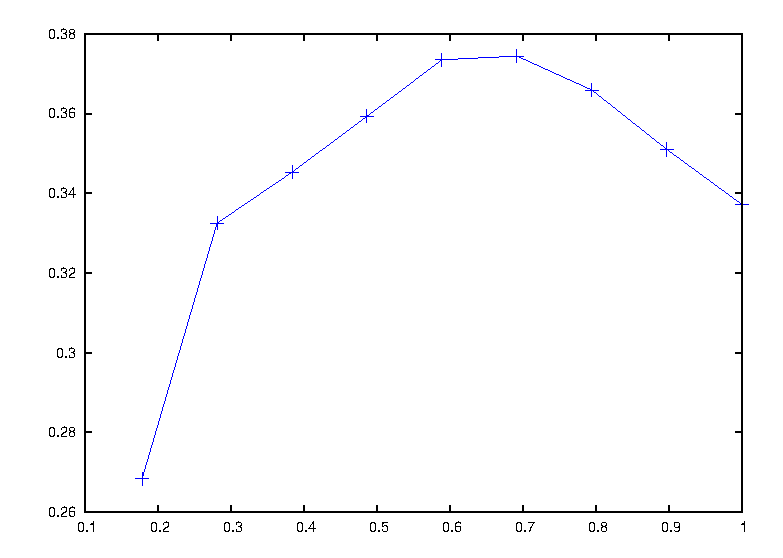
\includegraphics[width=0.73\textwidth,angle=-90]{figures/alphaomega-1.eps}
  \end{minipage} 
  \hfill
  \begin{minipage}[t]{0.49\textwidth}
  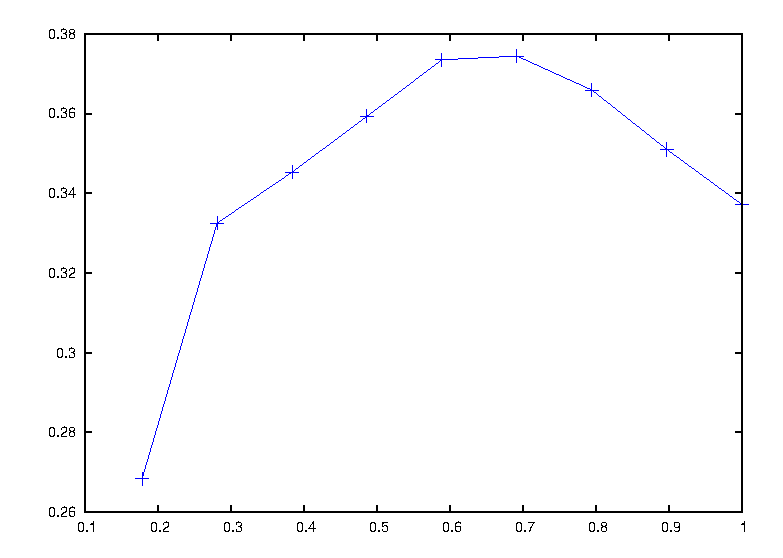
\includegraphics[width=0.73\textwidth,angle=-90]{figures/alphaomega-2.eps}
  \end{minipage}
  \caption{Relationship between $\omega$ and $\alpha^\omega_P\alpha^omega_D$
           in two iterations of problem {\tt capri}.}
  \label{fig:alphaomega}
\end{figure}

In our crude linesearch procedure we choose 9 points uniformly 
distributed in the interval $[\alpha_P\alpha_D, 1]$ 
and evaluate, for each of these points, the stepsizes 
$\alpha^\omega_P$ and $\alpha^\omega_D$ in both spaces. 
When a larger stepsize $\alpha^\omega_P$ or $\alpha^\omega_D$ is obtained, 
the corresponding $\omega$ is stored as $\omega_P$ or $\omega_D$ 
respectively. Hence, we allow two different weightings for directions 
in the primal and dual spaces.

%
% Section
%
\section{Numerical results}
\label{NumRes}

We have implemented our proposal within the HOPDM interior point solver 
\cite{HOPDM}. 
%
%Unlike Mehrotra and Li's approach, which generates Krylov directions and
%chooses weights and combines them into a composite direction, we
%generate a sequence of multiple centrality correctors.
%
We tested our implementation in a series of computational 
experiments, using test problems from different collections. 
As a comparison, we present the results obtained by PCx \cite{PCx}, 
a reference implementation of interior point methods. Since the two 
implementations, PCx and HOPDM, have different termination criteria 
in their default configurations, for the purpose of consistency,
in the results shown, 
we decided to implement in HOPDM the criteria used in the study 
performed by Mehrotra and Li \cite{MehrotraLi}.
Therefore, for all solvers optimal termination occurs when the conditions
(\ref{eq:TerminationCriteriaPCx}) are met, with feasibility
accuracy $p=8$ and complementarity accuracy $q = 10$.

We use $\gamma = 0.1$ in the definition of symmetric 
neighbourhood and define aspiration levels for the stepsizes using the rule
\[
  \tilde{\alpha}_{P} = \min(1.5 \alpha_{P} \! + \! 0.3, \, 1) 
  \quad \mbox{ and } \quad
  \tilde{\alpha}_{D} = \min(1.5 \alpha_{D} \! + \! 0.3, \, 1). 
\]
The values suggested in \cite{Gondzio96} were more conservative:
$\tilde{\alpha} = \min (\alpha + 0.1, \, 1)$.
Thanks to the weighting mechanism we can control 
the contribution of the corrector in an adaptive way,
and thus be more demanding in the definition of the aspired stepsizes.

Centrality correctors are accepted in the primal and/or dual space
if ${\alpha}_{P}^{new} \geq 1.01 \alpha_{P}$ 
and/or ${\alpha}_{D}^{new} \geq 1.01 \alpha_{D}$, respectively.

\fb{
Note that this is different from what described in \cite{Gondzio96}: there, 
a corrector is accepted if ${\alpha}^{new} \geq \alpha + \gamma\delta_\alpha$, 
where $\gamma = \delta_\alpha = 0.1$. What did HOPDM use to do?
}

We present our results in terms of number of iterations and number 
of backsolve operations. The rationale behind this decision is that 
the multiple centrality correctors technique determines the number 
of allowed correctors on the basis of the ratio between factorisation 
cost and backsolve cost. This ratio can be very different across 
implementations, and is mainly influenced by the linear algebra 
routines used. 
HOPDM comes with an in-house linear algebra implementation, while
PCx relies on the more sophisticated sparse Cholesky solver
of Ng and Peyton. Therefore, the PCx code tends to use less 
correctors per iteration.
In all other respects, the correction scheme follows closely the one
of HOPDM and the paper \cite{Gondzio96}.

%
%
\subsection{Mehrotra-Li test collection}
\label{ML-tests}

First we considered the test set used in \cite{MehrotraLi}: 
it contains 101 problems from both Netlib and Kennington collections. 
%
In Table~\ref{MLtotals} we present the computational comparison 
outlining the total number of iterations and the total number 
of backsolves necessary to solve the problems in Mehrotra and Li's test set. 
Column HO displays the results obtained
by the previous implementation, while column dHO reports
the results obtained by the current implementation of weighted
correctors with a default choice of the number of centrality correctors. 
The last column presents the relative change between the two 
versions of HOPDM tested. 
As a reference, we also report in this table the overall
statistics of PCx (release 1.1) on these problems. Also for PCx we adopted
the termination criteria (\ref{eq:TerminationCriteriaPCx}),
with $p = 8$ and $q = 10$.
We found the number of backsolves by counting the number of calls 
to the functions {\tt IRSOLV()} and {\tt EnhanceSolve()}, for HOPDM and
PCx respectively.
%
\begin{table}[ht]
  \centering
  \begin{tabular}{|l|c||c|c|r|}\cline{2-5}
    \multicolumn{1}{c|}{}& PCx & HO & dHO &\multicolumn{1}{c|}{Change}\\ \hline
    Iterations       & 2114 & 1871  & 1445           &   -22.77\% \\ 
    Backsolves       & 4849 & 6043  & 5717           &   -5.39\%  \\
    Backsolves/iter. & 2.29 & 3.23  & 3.95           &   +22.29\% \\ \hline
  \end{tabular}
  \caption{Overall results obtained on Mehrotra and Li's test collection.}
  \label{MLtotals}
\end{table}
%
\\From Table~\ref{MLtotals} we first observe the very small number 
of backsolves per iteration needed by PCx. This is due to the fact 
that PCx allows the use of Gondzio's multiple centrality correctors 
only in 4 problems: {\tt dfl001}, {\tt maros-r7}, {\tt pds-10} and 
{\tt pds-20}.
%
Also we notice that when we allow an adaptive weighting 
of the correctors there is a tendency to use more correctors 
per iteration than previously. 
This happens because the weighting mechanism makes it more likely
to accept some correctors that otherwise would have been rejected
as too aggressive.
While this usually leads to a decrease 
in iteration count, it also makes each iteration more expensive.

In Table~\ref{TimeML} we detail the problems for which we obtained savings 
in computational time. Given the small dimension of most of the problems 
in the Netlib collection, we did not expect major savings. However, as the
problem sizes increase, we can see that the proposed way of evaluating and
weighting the correctors pays off. This led us to investigate further 
the performance of the proposed implementation, which we will discuss
in Section~\ref{BN-tests}.
%
\begin{table}[ht]
  \centering
  \begin{minipage}[t]{0.36\textwidth}
    \begin{tabular}{|l|r|r|}\hline
      Problem & \multicolumn{1}{c|}{HO} & dHO \\ \hline
      bnl1    &   0.36 &   0.25 \\
      d{f}l001& 150.63 & 114.80 \\
      maros-r7&   7.76 &   7.52 \\
      pilot   &   5.23 &   4.35 \\ \hline
    \end{tabular}
  \end{minipage}
  \begin{minipage}[t]{0.36\textwidth}
    \begin{tabular}{|l|r|r|}\hline
      Problem & \multicolumn{1}{c|}{HO} & dHO\\ \hline
      pilot87 &  12.62 &  11.88 \\ 
      pds-06  &  24.59 &  21.31 \\
      pds-10  &  96.57 &  79.29 \\
      pds-20  & 923.71 & 633.64 \\ \hline
    \end{tabular}
  \end{minipage}
  \caption{Problems that showed time savings (times are in seconds).}
  \label{TimeML}
\end{table}

We were particularly interested in comparing the results produced by our 
weighted correctors approach with those published in \cite{MehrotraLi}. 
%
%A full comparison is presented in Table~\ref{MLresults}.
%In terms of the number of iterations, Mehrotra and Li's scheme is extremely 
%promising. 
% However, only 13 problems out of 101 showed a reduction 
% in computing time when using 4 Krylov directions. 
%
In the tables of results presented in \cite{MehrotraLi}, the best 
performance in terms of iteration count is obtained by PCx4, which 
uses 4 Krylov subspace vectors. These directions are combined with 
an affine-scaling predictor direction and Mehrotra's second-order 
correction, leading to 6 backsolves per iteration. 
%  {\bf (but it's not clear that they use Krylov 
%        directions and solve a linear subproblem at every iteration)}
This number increases when the linear subproblem produces an optimal 
objective value smaller than a specified threshold or the new iterate 
fails to satisfy some neighbourhood condition: in these cases 
the pure centering direction $\Delta_{cen}$ also needs to be computed,
and a seventh backsolve is performed.

As we understand the paper \cite{MehrotraLi}, PCx0 uses exactly 
2 backsolves per iteration: one to compute the affine-scaling direction,
another to compute Mehrotra's corrector; PCx2 and PCx4 compute 
two and four additional Krylov vectors, hence they use
4 and 6 backsolves per iteration, respectively.
In columns HO-0, HO-2 and HO-4, we present 
the results obtained by HOPDM when forcing the use of 0, 2 and 4 
multiple centrality correctors. 
In the column called HO\raisebox{1pt}{-$\infty$} we report the results 
obtained when an unlimited number of correctors is allowed
(in practice we allow no more than 20 correctors).
The last column, labelled dHO, presents the results obtained 
by the default way of choosing the number of correctors allowed.

Consequently, up to 2, 4 and 6 backsolves per iteration are allowed
in PCx0, PCx2 and PCx4 and in HO-0, HO-2 and HO-4 runs, respectively.
The number of backsolves reported for HOPDM includes two needed by 
the initialisation procedure: the number of backsolves 
should not exceed $2 \times {\rm {Its}} + 2$, 
$4 \times {\rm {Its}} + 2$ and $6 \times {\rm {Its}} + 2$ respectively
for HO-0, H0-2 and H0-4.
The observed number of backsolves is often much smaller
than these bounds because the correcting mechanism switches off 
when the stepsizes are equal to 1 or when the corrector does not 
improve the stepsize. Problem {\tt afiro} solved by HO-4 needs 24 
backsolves, 22 of which compute different components of directions, 
hence the average number of backsolves per iteration is only 22/6 
and is much smaller than 6. Occasionally,
as a consequence of numerical errors, certain components 
of direction are rejected on the grounds of insufficient accuracy:
in such case the number of backsolves may exceed the stated upper bounds.
The reader may observe for example that {\tt pilot4} is solved by HO-4
in 16 iterations, but the number of backsolves is equal to 100 and 
exceeds $6 \times 16 + 2 = 98$.

The version HO\raisebox{1pt}{-$\infty$} requires 1139 iterations to solve 
the collection of 101 problems, an average of just above 11 iterations
per problem. This version has only an academic interest, 
yet it reveals a spectacular efficiency of interior point 
methods which can solve difficult linear programs of medium sizes 
(reaching a couple of hundred thousand variables) in just 
a few iterations.
In particular, it suggests that if we had a cheap way of generating
search directions, then it would be beneficial to have as many as possible.

%
%
\subsection{Beyond Netlib}
\label{BN-tests}

We have applied our algorithm to examples from other test collections 
besides Netlib.
These include other medium to large linear programming problems, 
stochastic problems and quadratic programming problems.

We used a collection of medium to large problems taken from different
sources: problems {\tt CH} through {\tt CO9}
are MARKAL (Market Allocation) models; {\tt mod2} through {\tt worldl} are
agricultural models used earlier in \cite{Gondzio96}; problems {\tt route}
through {\tt rlfdual} can be retrieved from 
\begin{center}
{\tt http://www.sztaki.hu/\~{}meszaros/public\_ftp/lptestset/misc/},
\end{center}
problems {\tt neos1} through {\tt fome13} can be retrieved from 
\begin{center}
{\tt ftp://plato.asu.edu/pub/lptestset/}.
\end{center}

In Table~\ref{TimeBN} we detail the sizes of these problems and provide 
a time comparison between our previous implementation (shown in column
HO), and the current one (in column dHO).
This test collection contains problems large enough 
to show a consistent improvement in CPU time: in only 4 problems 
({\tt mod2}, {\tt dbc1}, {\tt watson-1}, {\tt sgpf5y6}) 
we recorded a deterioration of the performance by more than 1 second.
The improvements are significant on problems with a large 
number of nonzero elements. In these cases, dHO
produces savings from about 10\% to 30\%, with the remarkable results
in {\tt rail2586} and {\tt rail4284}, for which the relative savings 
reach 45\% and 65\%, respectively.

More numerical results obtained on some collections of stochastic
programming problems and quadratic problems can be found in
\cite{ColomboGondzio05}.

\begin{small}
\begin{longtable}{|l|rrr|r|r|r|} \hline 
  \multicolumn{1}{|c|}{Problem}
& \multicolumn{1}{c}{Rows}
& \multicolumn{1}{c}{Cols}
& \multicolumn{1}{c|}{Nonzeros}
& \multicolumn{1}{c|}{HO}
& \multicolumn{1}{c|}{dHO}
& \multicolumn{1}{c|}{Change}\\ \hline
\endhead
\hline
\multicolumn{7}{c}{\raisebox{-1ex}{Table~\ref{TimeBN}: Time comparison on 
other large problems (times are in seconds).}}
\endfoot
\label{TimeBN}
CH & 3852 & 5062 & 42910 & 1.03 & 1.23 & 19.4\% \\
GE & 10339 & 11098 & 53763 & 5.72 & 5.46 & -4.5\% \\
NL & 7195 & 9718 & 102570 & 4.37 & 3.95 & -9.6\% \\
BL & 6325 & 8018 & 58607 & 2.15 & 2.14 & -0.5\% \\
BL2 & 6325 & 8018 & 58607 & 2.35 & 2.31 &  -1.7\% \\
UK & 10131 & 14212 & 128341 & 2.48 & 3.21 &  29.4\% \\
CQ5 & 5149 & 7530 & 83564 & 2.54 & 2.60 &  2.4\% \\
CQ9 & 9451 & 13778 & 157598 & 9.67 & 8.84 &  -8.6\% \\
CO5 & 5878 & 7993 & 92788 & 3.16 & 3.59 &  13.6\% \\
CO9 & 10965 & 14851 & 176346 & 21.10 & 15.35 & -27.3\% \\
mod2 & 35664 & 31728 & 220116 & 20.59 & 21.68 & 5.3\% \\
world & 35510 & 32734 & 220748 & 26.35  & 23.41 & -11.2\% \\
world3 & 36266 & 33675 & 224959 & 31.13 & 27.49 & -11.7\% \\
world4 & 52996 & 37557 & 324502 & 73.21 & 56.14 & -23.3\% \\
world6 & 47038 & 32670 & 279024 & 39.33 & 32.79 & -16.6\% \\
world7 & 54807 & 37582 & 333509 & 43.14 & 36.02 & -16.5\% \\
worldl & 49108 & 33345 & 291942 & 43.95 & 36.82 & -16.2\% \\
route & 20894 & 23923 & 210025 & 40.92 & 33.78 & -17.4\% \\
ulevi & 6590 & 44605 & 162207 & 9.04 & 9.55 & 5.6\% \\
ulevimin & 6590 & 44605 & 162207 & 16.52 & 16.46 & -0.4\% \\
%aircraft & 3754 & 7517 & 24034 & 0.28 & 0.32 &  14.3\% \\
dbir1 & 18804 & 27355 & 1067815 & 162.18 & 146.51 & -9.7\% \\
dbir2 & 18906 & 27355 & 1148847 & 208.93 & 156.11 & -25.3\% \\
dbic1 & 43200 & 183235 & 1217046 & 72.96 & 77.31 & 5.9\% \\
pcb1000 & 1565 & 2428 & 22499 & 0.26 & 0.33 & 26.9\% \\
pcb3000 & 3960 & 6810 & 63367 & 1.13 & 1.16 & 2.7\% \\
rlfprim & 58866 & 8052 & 265975 & 15.63 & 15.08 & -3.5\% \\
rlfdual & 8052 & 66918 & 328891 & 71.17 & 49.79 & -30.0\% \\
neos1 & 131581 & 1892 & 468094 & 169.11 & 141.89 & -16.1\% \\
neos2 & 132568 & 1560 & 552596 & 113.86 & 86.13 & -24.4\% \\
neos3 & 132568 & 1560 & 552596 & 132.02 & 120.59 & -8.7\% \\
neos & 479119 & 36786 & 1084461 & 1785.80 & 1386.58 & -22.4\% \\
watson-1 & 201155 & 383927 & 1053564 & 138.60 & 166.21 & 19.9\% \\
sgpf5y6 & 246077 & 308634 & 902275 & 49.58 & 64.45 & 30.0\% \\
stormG2-1000 & 528185 & 1259121 & 4228817 & 1661.54 & 1623.19 & -2.3\% \\
rail507 & 507 & 63009 & 472358 & 9.77 & 10.10 & 3.4\% \\
rail516 & 516 & 47311 & 362207 & 7.59 & 5.89 & -22.4\% \\
rail582 & 582 & 55515 & 457223 & 9.67 & 9.60 & -0.7\% \\
rail2586 & 2586 & 920683 & 8929459 & 1029.36 & 566.82 & -44.9\% \\
rail4284 & 4284 & 1092610 & 12372358 & 2779.63 & 978.48 & -64.8\% \\
fome11 & 12142 & 24460 & 83746 & 407.20 & 265.21 & -34.9\% \\
fome12 & 24284 & 48920 & 167492 & 766.96 & 508.61 & -33.7\% \\
fome13 & 48568 & 97840 & 334984 & 1545.05 & 990.62 & -35.9\% \\
%\hline Totals  & & & & 11537.03  & 7713.8 \\
\end{longtable} 
\end{small}

In Figure~\ref{fig:PerfProfile}, we show the CPU-time based 
performance profile \cite{DolanMore} for the two algorithms. 
This graph shows the proportion of problems that each algorithm
has solved within $\tau$ times of the best. Hence, for
$\tau = 1$ it indicates that dHO has been the best solver on 72\%
of the problems, against 28\% for HO. For larger values of $\tau$,
the performance profile for dHO stays above the one for HO, thus
confirming its superiority. In particular, it solves all problems
within 1.3 times of the best.
%
\begin{figure}[ht]
  \centering
  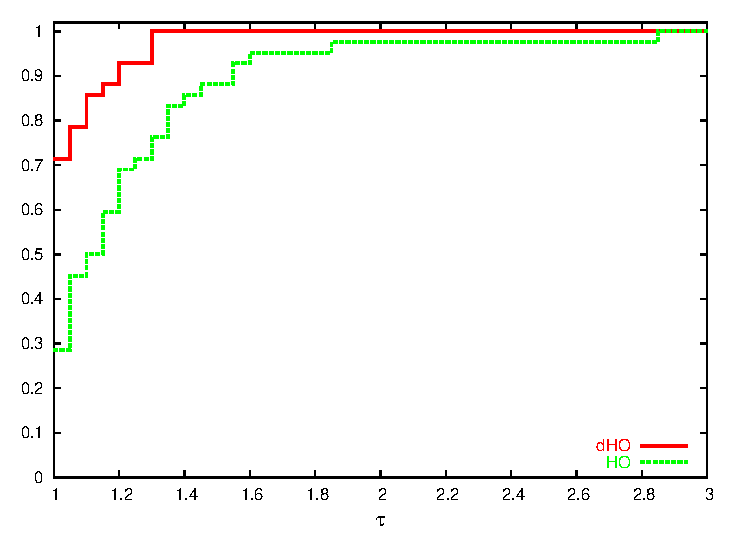
\includegraphics[width=0.75\textwidth]{figures/perfprof-BN.eps}
  \caption{Performance profile for HO and dHO on the set of problems
    of Table~\ref{TimeBN}.}
  \label{fig:PerfProfile}
\end{figure}

% The collection of stochastic programming problems contains 119 examples
% and comes from
% \begin{center}
% {\tt http://www.sztaki.hu/\~{}meszaros/public\_ftp/lptestset/stochlp/}. 
% \end{center}
% 
% We have also tested the implementation on a collection of 29 quadratic 
% programming problems, available from
% \begin{center}
% {\tt http://www.sztaki.hu/\~{}meszaros/public\_ftp/qpdata/}.
% \end{center}
%
% Normally, HOPDM automatically chooses between direct and iterative 
% approaches for computing directions. A higher-order correcting scheme
% makes much more sense with the direct approach when 
% backsolve is significantly less expensive than the factorisation.
% In order to maintain consistency, we forced HOPDM to use a direct 
% approach when 
% solving this class of problems, rather than an iterative scheme.

%
% Section
%
\subsection{Conclusions}
\label{Conclusions}

In this paper we have revisited the technique of multiple centrality 
correctors \cite{Gondzio96} and added a new degree of freedom to it. 
Instead of computing the corrected direction from 
$\Delta = \Delta_p + \Delta_c$ where $\Delta_p$ and $\Delta_c$ are 
the predictor and corrector terms, we allow a choice of weight 
$\omega \in (0,1]$ for the corrector term and compute 
$\Delta = \Delta_p + \omega \Delta_c$.
We combined this modification with the use of a symmetric neighbourhood
of the central path. We have shown that the use of this neighbourhood
does not cause any loss in the worst-case complexity of the algorithm. 

The computational results presented for different classes of problems 
demonstrate the potential of the new scheme. We have compared our algorithm 
against the recently introduced Krylov subspace scheme \cite{MehrotraLi}.
The two approaches have similarities: they look for a set of attractive 
independent terms from which the final direction is constructed. 
Mehrotra and Li's approach uses the first few elements from the basis
of the Krylov space; our approach generates direction terms using 
centrality correctors of \cite{Gondzio96}. Mehrotra and Li's approach 
solves an auxiliary linear program to find an optimal combination 
of all available direction terms; our approach repeatedly chooses 
the best weight for each newly constructed corrector term (and switches 
off if the use of the corrector does not offer sufficient improvement). 
Eventually, after adding $k$ corrector terms, 
the directions used in our approach have form
\[
\Delta = \Delta_a + \omega_1\Delta_1 + \ldots + \omega_k\Delta_k,
\]
and the affine-scaling term $\Delta_a$ contributes to it without any
reduction. Hence, the larger the stepsize, the more progress we make
towards the optimizer.

The comparison presented in Section~\ref{ML-tests} shows a clear advantage 
of our scheme over that of \cite{MehrotraLi}. Indeed, with the same 
number of direction terms allowed, our scheme outperforms Krylov subspace 
correctors by a wide margin. Multiple centrality correctors show 
consistent excellent performance on other classes of problems
including medium to large scale linear programs beyond the Netlib 
collection and medium scale quadratic programs.

\fb{
Monteiro, Adler and Resende \cite{MonteiroAdlerResende90} talk about
corrector steps.
}

\fb{
It would be good to try and implement using the search direction from
the previous iteration as another (free) direction to span the subspace.
}

\begin{remark}
From the study of subspace searches it is clear that the more 
directions we consider, the better the final search direction 
we get. Therefore, if we had a cheap way of generating search
directions (rather than from solving a system of linear equations),
then these should be employed.
\end{remark}

\begin{remark}
Mehrotra and Li \cite{MehrotraLi} mention employing previous search
directions alongside the usual ones. The use of these incurs an
increased memory usage, but no additional computational cost.
However, it does not seem that they were actually employed in
the runs. This opens some questions on what constitutes a valid
previous direction (only affine scaling, the final composite direction
or something else).
\end{remark}


\chapter[Warm-start strategies for stochastic linear programs.]{Warm-start strategies for \\stochastic linear programs.}
%Started on Monday 28 August 2006
%Aug: 29, 30
%Sep:  7,  8, 13
% 2007
%Feb:  4
%Mar:  8, 18, 19, 20, 28, 30
%Apr:  2

%
% Chapter: Warm-start
%
\label{ch:Warmstart}

In this chapter we develop an efficient way of constructing a 
starting point for structured large-scale stochastic linear programs.
We first present the relevant
concepts of stochastic programming and review some studies on 
warm-start techniques for interior point methods. Then we introduce 
the proposed method of generating an advanced starting point for 
stochastic programming that exploits the inherent structure of the
problem. Finally, we present an analysis of the warm-start strategy.
The results presented in this chapter have been the subject
of a joint work with Jacek Gondzio and Andreas Grothey
\cite{ColomboGondzioGrothey06}. 


%
% Section
%
\section{Stochastic programming}

Stochastic programming \cite{BirgeLouveaux,KallWallace}
is a technique to help decision-making 
in many areas of applied mathematics, logistics, engineering, economics and 
finance where some parameters are unknown.

\ignore{
In a large scenario tree there may be very little difference among 
scenarios, and so the large-scale problem can provide a fine-grained 
solution to a problem that could have been solved more coarsely by 
using a much smaller tree. This observation suggests a
warm-start technique that can be applied in the context of interior 
point methods. A warm-start solution is obtained by solving the 
stochastic optimization problem for a reduced event tree, whose 
dimension is much smaller than that of the complete one. The solution 
to the reduced problem is used to construct an advanced iterate for 
the complete formulation. We provide evidence that this novel way 
of exploiting the problem structure to generate an initial point 
provides a better iterate (in terms of centrality, feasibility, 
and closeness to optimality) than the one produced by a generic 
strategy.
}

By stochastic programming, we mean decision and control models in which 
data evolves over time, and are subject to significant uncertainty.
%
Uncertainty in the data is a commonly observed phenomenon in
optimization problems coming from applications. Uncertainty
affects problems that aim to plan future actions based on forecasted
prices or costs. In can be argued that nearly all practical
optimization problems display uncertainty in the data, even if this is
not made explicit in the chosen solution method. 

\ignore{
A crude approach to the problem of optimization under uncertainty
has been to replace the uncertain data by their expected value and
solve an {\em average case} problem. However, this approach is not
suitable when some sort of provision of hedging against risk has to be
taken into account. Another popular approach is {\em Robust
optimization}, or the optimization of the {\em worst case}
scenario \cite{KallWallace}. 
}

When the uncertainty cannot be conveniently forecasted, the use of 
deterministic models is considered inadequate for decision making. In 
these situations, being able to describe and model the uncertain parameters
becomes a requirement for robust decision making. Stochastic 
programming is the discipline that 
studies the methods and provides the tools for modelling uncertainty.

Stochastic programming models uncertainty through the analysis 
of possible future outcomes (scenarios). The 
robustness of the decisions taken increases with the detail of the 
description, which requires generating very large scenario trees.
Stochastic programming aims to take all possible future scenarios 
into account, weighting them
with their respective probabilities. Its strength lies in the
adaptability which allows to express preferences such as restricting
the exposure to risk. Unlike alternative approaches, it allows to model
situations in which possible future events are correlated or follow a
time-structure, in that realisations become known in stages and it is
possible to react to the observed events.

Taking into account a large number of possible scenarios leads
to the generation of large-scale structured optimization problems.
With the growing industrial acknowledgement of the benefits of 
considering uncertainty for planning purposes, it is expected that the 
need for solving very large instances will grow as well.

Its perceived weaknesses are the need for reliable forecasts
of the probabilities of the future events under consideration
(which may not be available), and the fact that stochastic programming
(especially when applied to multi-stage models) tends to lead to
problems with very large dimensions, thus making their solution
challenging. 

As the dimensions of the problems increase, the computational advantages 
of relying on interior point solvers become more and more evident. 
Very-large-scale problems, however, create more than one difficulty to general 
purpose solvers.
Problems of such sizes can be solved provided they are not only sparse,
but also structured. If that is the case, then the structure present 
in the matrix should be conveniently exploited.
The easier access to powerful parallel machines leads to a 
further advantage coming from assigning the computational work 
to more than one processing unit through the parallelisation of 
the linear algebra.

%
%
\subsection{Stochastic programming concepts}

A stochastic programming problem incorporates the uncertain parameters
in the model. 
Following \cite{BirgeLouveaux}, this can be illustrated by the 
{\em two-stage stochastic problem}
%
\be  \label{eq:SP1}
  \begin{array}{rl}
    \min        & c^T x + \E_\xi Q(x, \xi) \\
    \mbox{s.t.} & Ax = b,  \\
                & x\geq 0, \\
  \end{array}
\ee
%
where $\xi$ is a random variable and $\E_\xi$ is the expectation function
and
\be  \label{eq:SP2}
  \begin{array}{rcrl}
  Q(x, \xi) &\!\!\! = \!\!\! & \min & q(\xi)^T y(\xi) \\
            &   & \mbox{s.t.} & Wy(\xi) = h(\xi) - T(\xi)x, \\
	    &   &             & y(\xi) \ge 0.
  \end{array}
\ee
This can be interpreted as an optimization
problem in which some parameters or coefficients are unknown.
While (\ref{eq:SP1}) models the first stage decisions, 
(\ref{eq:SP2}) refers to the second stage decisions, which can
be made only after a realisation of the random variable $\xi$
has become known. Note how the first-stage decision variables $x$ 
appear in (\ref{eq:SP2}): at the time when the realisation
become available, the first-stage decisions have already been made.

\ignore{
Formulation (\ref{eq:SP}) is however an unsatisfactory model, since
it is unclear how to interpret the probabilistic constraint
$g(x,\xi) \le 0$. A better formulation is the stochastic program
with recourse:
\begin{eqnarray} \label{eq:SPRecourse}
\min_x \hspace{-1.5em} && \E_\xi[f(x, \xi) + Q(x, \xi)] \nonumber \\ 
  && Q(x,\xi) = \min_y \{\, q(y) : u_i(y) \ge g_i^+(x, \xi),\:\forall i \,\},\\
  && g_i^+(x, \xi) = \max \{\, g_i(x, \xi), \, 0 \,\}. \nonumber
\end{eqnarray}
}

In stochastic programming, the uncertain environment is 
described through a stochastic process which is assumed to be 
known or can be either estimated from historical data or 
conjectured according to some prescribed properties. The 
continuous process $\xi$ is usually further approximated by a discrete 
distribution, $\xi \in \{\xi_1, \ldots,\xi_n\}$, $p(\xi=\xi_i) = p_i$,
in order to obtain a computationally amenable description. 
%
In such a case, the most common technique generates a 
finite, but usually very large, number of scenarios that represent an 
approximate description of the possible outcomes.

%The decision variables $x$ are
%split depending on the timing of the decision: $x_0$ are those
%variables whose value is to be decided {\em before} the random event
%becomes known, $x_i$ are decisions taken as a reaction to the outcome
%of $\xi$ being $\xi_i$ (recourse action). Problem
%(\ref{continuousSP}) then becomes
%\begin{equation}
%\min_{x} \sum_{i=1}^n p_i f(x_0, x_i, \xi_i)) \text{~subject
%to~}c(x_0, x_i, \xi_i) \le 0,
%\label{SP}
%\end{equation}

The model can be generalised to a {\em multi-stage model} in which 
the evolution of uncertainties can be 
described as an alternating sequence of decisions and random 
realisations that occur at different stages.
A multi-stage stochastic program with recourse is a multi-period 
mathematical program where parameters are assumed to be uncertain 
along the time path.

The stages do not necessarily refer to time periods, but they correspond
to steps in the decision process. In particular, at each stage the
realisations of some random parameters become known, and a decision
must be taken.
The main interest lies in the 
first-stage decisions which consist of all decisions that have to
be made before the information is revealed. Later-stage decisions 
are allowed to adapt to the information that has become available 
up to that point.

The discrete stochastic process can be represented as an event tree,
where each node denotes a stage when a realisation 
of the random process becomes known and a subsequent decision is taken.
A path from the root to a leaf node of the event tree represents a 
scenario.
A very simple event tree is shown in Figure~\ref{fig:EventTree}.
%
\begin{figure}[ht]
  \begin{center}
    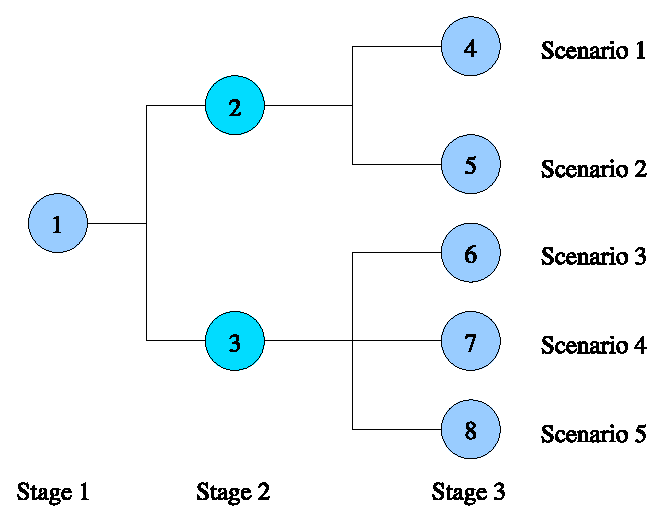
\includegraphics[scale=0.6]{figures/tree.eps}
    \caption{Event tree.}
    \label{fig:EventTree}
  \end{center}
  \vspace{-3ex}
\end{figure}

To each node of the event tree we associate a set of constraints, an 
objective function, and the conditional probability of visiting the 
node from its parent node in the previous stage.
The probability of each scenario is the product of the 
conditional probabilities of visiting each node on the path.

It should be noted that usually a very large number of scenarios is
needed to adequately capture the characteristics of the underlying
continuous distribution, particularly in the multi-stage setting.
In this case, the number of scenarios grows exponentially with the
number of decisions considered at each stage.
The size of the scenario tree determines the size of the optimization
program.

The question of how to generate an appropriate scenario tree
is not trivial, and has received extensive attention in the
literature 
\cite{DupacovaConsigliWallace,HoylandKautWallace,HoylandWallace,Pflug01}.

%
%
\subsection{The deterministic equivalent formulation}
\label{DetEqForm}

A natural formulation of a stochastic programming problem relies on 
recursion to describe the dynamics of the modelled process.
The term {\it recourse} means that, at each stage, the decision 
variables adapt to the different outcomes of the random parameters.
For ease of presentation, we consider the linear version of the
recourse problem:
%
\be \label{eq:SLPRecourse}
\begin{array}{rl}
  \min & c^T x + \E_\xi[\min\, q(\xi)^T y(\xi)]     \\
  \text{s.t.} &  Ax                       = b,      \\
	      &  T(\xi) x + W(\xi) y(\xi) = h(\xi), \\
	      &  x \geq 0,\; y(\xi) \ge 0,
\end{array}
\ee
%
where $y(\xi)$ denotes the recourse action which depends on the 
outcome of the random process $\xi$. 
Note that (\ref{eq:SLPRecourse}) combines in a single formulation
both (\ref{eq:SP1}) and (\ref{eq:SP2}).
After discretizing $\xi$ 
according to $P(x^i=\xi_i) = p^i$, and using the notation 
$T^i = T(\xi_i)$ (and analogously for $h^i$, $W^i$, $y^i$ and $q^i$), 
problem (\ref{eq:SLPRecourse}) can be written in the 
{\em deterministic equivalent formulation}:
\be \label{eq:DetEq-2stage}
\begin{array}{rlllll}
\min & c^T x + \sum_i p^i(q^i)^T y^i \\
\mbox{s.t.} & Ax              &        &          & = b,   \\
            & T^1 x + W^1 y^1 &        &          & = h^1  \\
	    & \quad\vdots     & \hspace{-1em}\ddots & & \;\vdots \\
            & T^n x           &        &+\; W^n y^n & = h^n \\
            & x \geq 0,\; y^i \ge 0.
\end{array}
\ee
The deterministic equivalent formulation is derived by writing
explicitly each possible realisation of the random parameters.
The formulation (\ref{eq:DetEq-2stage}) does not have any stochasticity
left, but is completely deterministic, and is therefore a common
linear programming problem of (very) large dimensions.
Also note that problem (\ref{eq:DetEq-2stage}) displays a
dual-block angular structure
in the constraint matrix.

\fb{
Make a step from two-stage to multistage.
}

To formulate the deterministic equivalent of the multi-stage 
stochastic programming problem we first need to enumerate all nodes 
of the event tree. We use a breadth-first 
search order, i.e., we start from a root node corresponding 
to the initial stage and end with leaf nodes corresponding 
to the last stage. In this case, the constraint matrix displays
a nested dual-block angular structure.

Let $t = 1,2,\ldots,T$ denote the stage and $l_t$ be the index of a 
node at stage $t$.
Let $L_t$ denote the last node at stage $t$. Hence 
the nodes that belong to stage $t > 1$ have indices 
$l_t = L_{t-1} \! + \! 1, L_{t-1} \! + \! 2, \dots, L_t$. 
For any node in the tree at stage $t$ there is only one immediate
ancestor at stage $t-1$ and a finite number of descendants at $t+1$.
With $a(l_t)$ we denote the direct ancestor of node $l_t$ (which is a 
node that belongs to stage $t-1$).
All decision variables $x$ are superscripted with the node number 
$l_t$.

The main constraint that describes the dynamics of the system has the form 
\[
  T^{l_t}x^{a(l_t)} +W^{l_t}x^{l_t} =h^{l_t}, \qquad l_t =L_{t-1}+1,\dots,L_t,
\]
%
where $T^{l_t}$ is the technology matrix that varies 
with the node in the event tree, and $W^{l_t}$ is the recourse
matrix that, in general, depends on realisations within the same stage,
but often varies only with time.

The deterministic equivalent formulation of the multi-stage 
problem has the following general form:
\begin{equation}
  \begin{array}{rrclll}
    \min & (q^{l_1})^T x^{l_1} & + & \!\!\!\!{\displaystyle \sum_{l_2=L_1 \!+\! 1}^{L_2}} \!\!\! p^{l_2} (q^{l_2})^T x^{l_2} && \!\!\!\!\!\!  + \; \ldots \; + {\displaystyle \sum_{l_T = L_{T-1} \! + \! 1}^{L_T}} \!\!\!\!\! p^{l_T} (q^{l_T})^T x^{l_T} \\
    \mbox{s.t.} & & & W^{l_1} x^{l_1} & \hspace{-1.5cm} = h^{l_1}, \\
    & T^{l_2} x^1 & + & W^{l_2} x^{l_2} & \hspace{-1.5cm} = h^{l_2}, & l_2 = L_1 \!+\! 1,\dots,L_2, \\
    & & \vdots & & \hspace{-1.4cm} \vdots \\
    & T^{l_T} x^{a(l_T)} & + &  W^{l_T} x^{l_T} & \hspace{-1.5cm} = h^{l_T}, & l_T = L_{T-1} \! + \! 1, \dots, L_T, \\
    & & & x^{l_t} & \hspace{-1.5cm} \geq 0, & l_t = 1,\dots, L_{T}. \\
    \label{DetEquiv}
  \end{array} 
\end{equation}

Note that the probabilities in the objective function of problem 
(\ref{DetEquiv}) are the unconditional path probabilities: $p^l$ is 
the probability that a path goes through node $l$, which equals the 
product of the conditional probabilities along the path from the root 
to the node $l$.

If the event tree is traversed with depth-first-search ordering of the 
nodes during the generation of the mathematical program, the 
corresponding constraint matrix displays a nested dual block-angular 
structure.
Figure~\ref{fig:deteq} displays the two possible structures 
for the event tree of Figure~\ref{fig:EventTree} according 
to the chosen ordering of nodes.
%
\begin{figure}[ht]
  \centering
    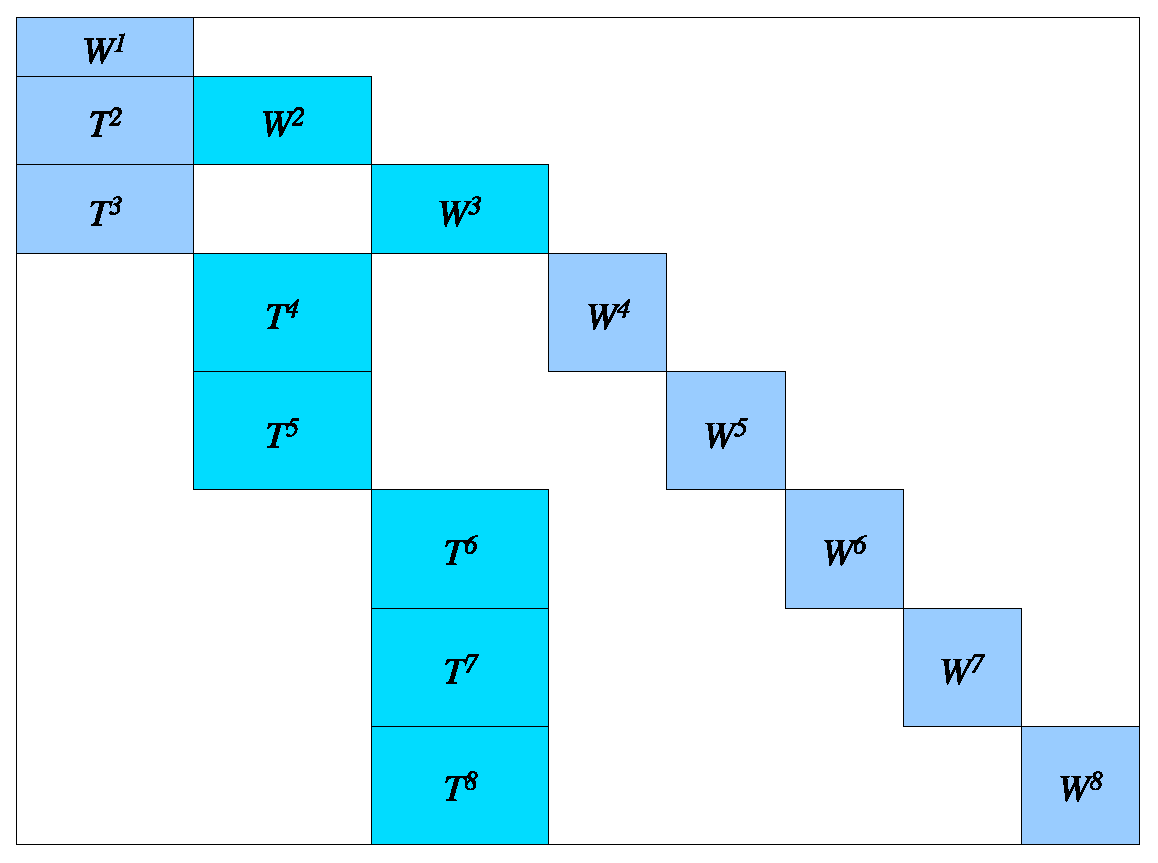
\includegraphics[scale=0.37]{figures/deteq-bfs.eps} \hfill
    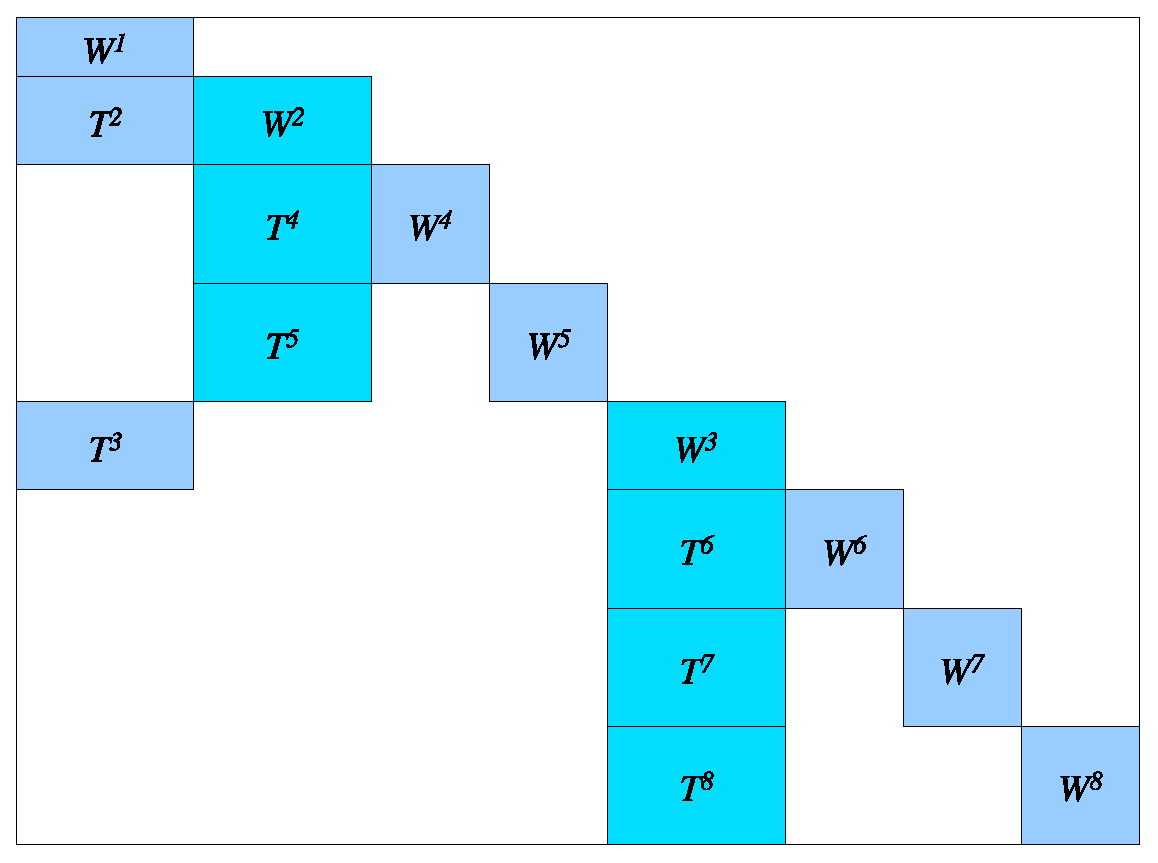
\includegraphics[scale=0.37]{figures/deteq-dfs.eps}
    \caption{Deterministic equivalent corresponding to the event tree 
             of Figure~\ref{fig:EventTree}, with nodes listed in breadth-first 
             order (left) and depth-first order (right).}
    \label{fig:deteq}
\end{figure}
%
While the different ordering of blocks whithin the matrix is not 
relevant for general-purpose solvers, the
structure-exploiting software \OOPS \cite{GondzioSarkissian} can take 
fully advantage of the nested structure.

Clearly, (\ref{DetEquiv}) represents a structured linear program. Its 
structure should be exploited in the solution algorithm.
Several solution methods for stochastic linear programs have been 
presented in the literature. These often rely on some decomposition
approach \cite{Birge85,MulveyRuszczynski,LinderothWright03}, among others.
Kall and Mayer \cite{KallMayer} provided a comparison of different
solution algorithms for stochastic linear programming problems.
In what follows, instead, we consider solving the deterministic equivalent
problem directly through an interior point method.

%
% Section
%
\section{Warm-start with interior point methods}
\label{sec:WarmStart}

Consider the linear programming problem in standard form
\be  \label{eq:CompleteProblem}
\min\;  c^T x \;\quad \mbox{s.t. }\; Ax = b, \;\; x \ge 0,
\ee
where $A \in \R^{m \times n}$ is full rank, 
$x, c \in \R^{n}$ and $b \in \R^{m}$. 
For the purposes of this paper, problem (\ref{eq:CompleteProblem})
corresponds to the deterministic equivalent generated from a
given event tree $\Ctree$, and we will refer to it as the 
{\em complete problem}.

As discussed in Section~\ref{sec:StartingPoint}, the problem of 
finding a starting point is usually solved by using 
Mehrotra's starting point heuristic \cite{Mehrotra92}, which is 
considered to be computationally effective for generic problems.

However, many practical applications rely on solving a sequence 
of closely related problems, where the instances differ by some 
perturbation. This happens within algorithms that are sequential 
in their nature, such as sequential linear programming or
sequential quadratic programming.
It is also very common in (mixed) integer programming, when the
problems are solved by relaxing the integrality constraints and
introducing some branching strategy, such as in branch-and-bound,
branch-and-cut, branch-and-price.
Similarly, sequential problems appear in the context of solution 
methods based on cutting planes.

In these situations, we expect the solution of an instance to be 
close to the solution of the next one, in the sense that some of
the information gathered in the solution process may still be valid. 
Therefore, starting the 
optimization of one problem from the solution of the previous instance
should reduce the computational effort of solving the perturbed instance.
The strategies that exploit and advanced starting point are called
{\em warm-start strategies}.

Warm-start techniques are very successful 
when implemented with a simplex solver (see, for example, 
\cite{Bixby02}). 

\fb{
More on the simplex.
}

However, in the context of interior point methods, it 
is much more difficult to implement successfully, for the reasons
we outline below.

%
%
\subsection{Difficulties}
\label{sec:WarmStartDifficulties}

The optimal solution of a linear programming problem found with 
a path-following interior point methods is very close to a vertex of 
the feasible polytope or, in the more common case of multiple solutions, 
corresponds in the analytic center of the optimal set of solutions.
When the polytope changes (due, for example,
to the addition of cutting planes or other changes in the 
problem data), the optimal solution changes as well.
In such a case the previous solution is very close to a non optimal
vertex or, in other words, is very far from the central path
of the perturbed instance. 

As presented in Chapter~\ref{ch:Ipm}, interior point methods approach 
the solution to the KKT system of optimality conditions by relaxing 
the complementarity requirements and obtaining the perturbed
system (\ref{eq:PerturbedKKT}).
As moving towards a vertex can be interpreted as making 
a decision on the optimal partitioning, considering the 
system (\ref{eq:PerturbedKKT}) is equivalent to postponing 
the choice of the optimal partitioning.
If the vertex is not an 
optimal one, then the central path will not approach it.

The effectiveness of an interior point algorithm degrades when an 
iterate gets too close to a boundary before optimality is reached,
or, equivalently, when the iterate gets far from the central path.
In these situations the algorithm may spend many iterations in recovering
centrality, during which small steps are usually generated and thus
very slow progress is achieved.

Hipolito \cite{Hipolito} considered the issue of robustness of 
search directions in interior point methods in these situations.
While his analysis concerns the dual affine-scaling algorithm, 
it seems to provide an interesting insight on the misbehaviour
of the search directions computed from non-central points also
for primal--dual algorithms.
In his analysis, Hipolito showed that if the iterate is close 
to a boundary, the affine-scaling direction may be parallel to 
the nearby constraints. In such cases, the corrector direction 
may also display the same behaviour, and short stepsizes are 
obtained for the resulting combined search direction.

The required features for a good warm-start candidate for an
interior point algorithm are somewhat contradictory.
The point should not be too close to the boundary of the feasible 
region in order to be able to absorb larger perturbations in the 
problem data. 
Also, it should be sufficiently advanced to provide 
computational savings over a cold-start iterate.
These considerations lead to the idea of storing an approximate
$\mu$-center well before reaching optimality 
\cite{Gondzio98,GondzioGrothey03,GondzioVial,YildirimWright}.

The theory and practice of warm-start techniques for interior point 
methods is a relatively new and still open field of study.
In the remainder of this section we present a review of some 
of the warm-start approaches proposed in the interior point literature.

%
%
\subsection{Changes in the problem size}

Mitchell \cite{phd:Mitchell} and Mitchell and Todd \cite{MitchellTodd}
analyse the potential reduction interior point method within
a cutting plane algorithm. They exploit the fact that
the primal feasible point can be constructed after a set of new
columns is added to the problem. They use this strategy with success
in column generation scheme and more generally in the solution 
of combinatorial optimization problems.

Gondzio \cite{Gondzio98} presents a warm-start procedure for 
primal--dual interior point methods in the context of a cutting 
plane method. The interior 
point method is used to solve a sequence of restricted master 
problems, which differ by one or more cutting planes.
%
% Therefore, by construction the solution to one problem violates 
% some of the newly added constraints.
% The optimal solution to a problem is necessarily very close 
% to the boundary, thus is an unattractive starting point 
% for a perturbed problem. Therefore, an alternative warm-start 
% iterate needs to be defined.
%
The idea proposed in \cite{Gondzio98} is to store a nearly optimal 
point (3--4 digits of accuracy) to be employed as a warm-start point.
%
% Because of the cutting plane setting, the problem is then solved 
% to optimality (7--8 digits of accuracy) in order to generate 
% appropriate cuts.
%
As one requirement for a good iterate is centrality, it is of interest 
to perform a few centering steps on the stored iterate, the cost of 
which is marginal, as a factorisation is already available. The 
recentering steps proposed are based on
centrality correctors \cite{Gondzio96}.
An auxiliary feasibility recovery procedure may be needed as, due to 
the addition of cuts, large infeasibilities are often produced.

The role of interior point methods in integer and combinatorial 
optimization has been comprehensively surveyed in \cite{Mitchell96} 
and \cite{MitchellPardalosResende98}. This is relevant as these classes
of optimization problems are generally solved by formulating a sequence
of linear relaxations, where the problem instances differ by the
addition of cutting planes and facet-inducing constraints.

%
%
\subsection{Perturbations that do not affect the problem size}

Hipolito \cite{Hipolito} studies an alternative centering direction 
in the context of the dual affine-scaling algorithm. Such a 
direction is designed to move the iterate away from the boundary, 
overcoming the risk of moving parallel to it that was mentioned 
in Section~\ref{sec:WarmStartDifficulties}. 
By considering a weighted least squares formulation, Hipolito 
develops the dual affine-scaling and the corresponding Newton 
centering directions. 
This study has an immediate interest for warm-starting approaches,
as the resulting direction points towards the interior of the 
feasible region, thus providing the algorithm with the necessary 
space to make fast progress. 
Unfortunately, it is developed only for the dual affine-scaling 
algorithm, and to the best of our knowledge there have been no 
studies on how to obtain a similar search direction in the 
primal--dual context.

The warm-start approach proposed in \cite{Gondzio98} is extended
in \cite{GondzioVial} to the case of solving a sequence of problems 
with the same dimensions but changing problem data (the objective 
function or the right-hand side). Such situations arise 
in the context of decomposition approaches for large structured 
linear programs. 
In the case of Dantzig--Wolfe decomposition, successive subproblems 
differ only in the objective function, while in the case 
of Benders decomposition they differ only in the right-hand sides.
Following \cite{Gondzio98}, nearly optimal points are saved and used 
to warm start the solution of subsequent subproblems \cite{GondzioVial}.

% An advanced application of this technique is studied in 
% \cite{GondzioVial}, where a decomposition approach for large 
% structured linear programs is implemented within an interior point 
% framework. In this setting, a sequence of linear problems is generated 
% by adding cutting planes to provide a polyhedral approximation of a 
% non-differentiable convex function, and a warm-start strategy is 
% applied when solving each subproblem.

\yildirim and Wright \cite{YildirimWright} consider again the case 
of solving a sequence of problems in fixed dimensions, and
analyse the number of iterations required to converge to a 
solution of the perturbed instance from the warm-start point and 
obtain worst-case estimates.
They show that these estimates depend on the size of the perturbation 
as well as on the conditioning %and other properties 
of the problem 
instances. Thus they obtain conditions under which the complexity 
of the warm-start approach is better than for the cold start case.

The strategy proposed in \cite{YildirimWright} aims at absorbing the 
primal and dual infeasibilities introduced by the perturbation in just 
one step.
% relying on the centrality of the iterate from one instance
% to provide enough centrality for the starting point of the next instance.
This strategy requires to backtrack to an iterate for which $\mu$ is 
large enough to allow a full step for the correction direction they produce. 
The amount of necessary backtracking depends on the magnitude 
of the perturbation:
this is intuitively justified considering that a large perturbation 
will produce a large adjustment, and it is essential to guarantee that 
a full step will not compromise the positivity requirements of the 
iterate.
%
To ensure the availability of an approximate $\mu$-center from which 
the perturbation can be absorbed in one step, a subset of 
iterates for different values of $\mu$ is stored.
When the size of the perturbation becomes known, the closest $\mu$ 
available is retrieved, and the corresponding iterate is used as a 
warm-start point for the next problem in the sequence.
%
In \cite{YildirimWright}, two different corrections for the perturbation
are studied: one is based on least squares, the other on a Newton step 
correction.
A detailed computational comparison of these strategies has been 
carried out by John and \yildirim \cite{JohnYildirim}.

Gondzio and Grothey \cite{GondzioGrothey03} propose a different 
reoptimization technique for interior point methods.
As in \cite{YildirimWright}, they aim at obtaining conditions for 
perturbations that can be absorbed in one Newton step.
Hence, they introduce a relative measure of perturbations, in which 
the primal and the dual spaces are analysed independently.

%They derive the directions for absorbing primal and dual 
%infeasibilities from the system
%\[
%\left[ \begin{array}{ccc}
%    A & 0 & 0 \\ 0 &A^T & I \\ S & 0 & X
%  \end{array} \right]
%\left[ \begin{array}{c}
%    \Delta x \\ \Delta \lambda \\ \Delta s
%  \end{array} \right] = 
%\left[ \begin{array}{c}
%    -r_b \\ -r_c \\ 0
%  \end{array} \right].
%\]
%This formulation aims at restoring feasibility, while the requirement 
%for a well-centred iterate is considered separately. 

This reoptimization procedure is based on two phases: first, an attempt 
is made to absorb the infeasibilities caused by the perturbation with a full 
Newton step; second, the centrality of the iterate is improved. Another 
key feature of \yildirim and Wright's approach is that the primal search 
direction is governed only by the primal perturbation, and similarly 
for the dual space. This corresponds to solving the Newton system 
(\ref{eq:NewtonSystem}) for the two right-hand sides independently
%
\[
\left[ \begin{array}{ccc}
    A & 0 & 0 \\ 0 &A^T & I \\ S & 0 & X
  \end{array} \right]
\left[ \begin{array}{c}
    \Delta x \\ \Delta y \\ \Delta s
  \end{array} \right] = 
\left[ \begin{array}{c}
    \xi_b \\ 0 \\ 0
  \end{array} \right] +
\left[ \begin{array}{c}
    0 \\ \xi_c \\ 0
  \end{array} \right].
\]
%
They produce bounds on the magnitude of primal perturbation $\xi_b$ 
and dual perturbation $\xi_c$ that can be absorbed in a single 
Newton step. As opposed to the results of \cite{YildirimWright}, 
the bounds of \cite{GondzioGrothey03} are easy to compute and 
thus can be used in practice.

If the perturbation is bounded above by some quantity depending 
on $n$ and $\theta$, a full Newton step can be taken in the dual space. 
This happens for both the $\mathcal{N}_2$ and $\mathcal{N}_\infty$ 
neighbourhoods. Similarly, a full Newton step can be taken in the 
primal feasibility restoration direction. These conditions may not 
be satisfied in practice. In such case, a different iterate further 
away from optimality may be more likely to allow for a full Newton step.

A practical implementation is developed within an infeasible interior 
point method. In this context, a stronger emphasis may be put on 
reducing the infeasibilities. This is accomplished with additional 
centering steps.
An approximate $\mu$-center is stored for a tolerance level that 
depends on the magnitude of the expected perturbation. This does not 
exclude the possibility of storing a sequence of iterates, as proposed 
in \cite{YildirimWright}, thus postponing the choice of the one to 
use.
As the problem size does not change, an approximate $\mu$-center 
can immediately be used as an iterate for the next problem.
If only one iterate is stored, then the absorption of infeasibilities 
may be spread across a few iterations whenever the stepsizes fall 
below a predefined level.
As this strategy does not make assumptions upon the centrality of the 
warm-start iterate,
it can be initialised with any iterate.
Gondzio and Grothey \cite{GondzioGrothey03} apply this warm-start 
strategy successfully to structured problems for crash-start points that 
come from a cross-decomposition scheme, and thus may lack centrality.

A different approach has been studied by Benson and Shanno 
\cite{BensonShanno}. They investigate how to improve the efficiency 
of interior point methods in a reoptimization context by the use of 
a primal--dual penalty approach.
While standard penalty techniques are effective only in one space, 
the introduction of penalty parameters in both the primal and the 
dual problems allows to capture perturbations in both spaces.
%
For example, an $l_1$ penalty can deal with changes in the right-hand
side of the constraints (primal changes), but has virtually no effect
in perturbations of the objective coefficients (dual changes).

The strategy relaxes the non-negativity constraints for the decision
variables, penalising the violation in the objective, for both
the primal and dual problems.
The penalised problem allows the variables to become negative: 
this provides more freedom of movement for the variables, with
the immediate advantage of accepting larger stepsizes along 
the computed search direction. This favours a faster progress
especially in the first few iterations, when the perturbation needs
to be absorbed.
This is of particular importance in reoptimization, as the optimal
solution of the previous problem is necessarily close to a boundary.
%
Benson and Shanno \cite{BensonShanno} also provide some computational
evidence of the effectiveness of their strategy.

\hrulefill

Large or huge-scale problems, however, create more than one difficulty 
to general purpose solvers. Problems of these sizes can be solved by 
exploiting the structure present in the matrix. A further advantage 
comes from assigning the work to be done to more than one processing unit. 
This is where structure-exploiting parallel solvers such as \OOPS 
\cite{GondzioSarkissian} excel. Moreover, structure-exploiting interior 
point methods can be used not only for linear programming problems, 
but also for quadratic and nonlinear problems \cite{GondzioGrothey04}.


%
% Section
%
\section{A reduced-tree warm-start iterate}
\label{sec:ReducedTree}

While the strategies mentioned in the previous section apply to
general linear problems, we introduce an approach tailored to
stochastic programming. In particular, we propose to exploit the structure
inherent to a stochastic programming problem to generate a good 
warm-start iterate.

In the event tree corresponding to a large multistage program, 
the numerous leaf nodes descend from a relatively small number of 
branches in the first few stages. Two ``neighbouring'' scenarios, 
that is two scenarios that have common nodes, may display large 
differences concerning later stage decisions, but the decisions 
taken in the earlier stages are identical (nonanticipativity).
Moreover, there may be very little difference among 
scenarios, and so the large-scale problem can provide a fine-grained 
solution to a problem that could have been solved more coarsely by 
using a much smaller tree. 

These observations suggests a
warm-start technique that can be applied in the context of interior 
point methods. A warm-start solution is obtained by solving the 
stochastic optimization problem for a reduced event tree, whose 
dimension is much smaller than that of the complete one. The solution 
to the reduced problem is used to construct an advanced iterate for 
the complete formulation. We provide evidence that this novel way 
of exploiting the problem structure to generate an initial point 
provides a better iterate (in terms of centrality, feasibility, 
and closeness to optimality) than the one produced by a generic 
strategy.

Techniques for reducing the size of the scenario tree have been studied 
before from a probabilistic perspective; in some cases considerable 
savings can be obtained with such methods. Among others, 
Dupa\v{c}ov{\'a} \etal \cite{Dupacova} discuss an optimal scenario 
reduction technique that couples a large reduction of the scenario 
tree with a small loss in accuracy. In their example, a reduction by 
50\% of the scenario tree still maintains about 90\% of the original 
accuracy.
In this paper, we are interested in capturing some aspects of the 
stochasticity of the event tree without assuming further knowledge on 
the underlying stochastic process that generated it. Given this difference 
from what is required for example by \cite{Dupacova}, we will use less 
sophisticated arguments in finding a reduced tree.
We remark that if we have knowledge of the underlying stochastic process,
then we could exploit it in the generation of the reduced tree.

We first study how to build a reduced tree by choosing just 
some of the possible scenarios. We provide some insight on how to make 
this selection, so that our choice performs better than an arbitrary 
one.
Then we discuss how to obtain a warm-start solution from the reduced 
tree that corresponds to the chosen scenarios.
Our aim is to generate a warm-start iterate that allows to solve to 
optimality the complete problem in fewer iterations (and less computing 
time) than by a standard starting point heuristic \cite{Mehrotra92}.
With these aims, we propose a way of choosing a subset of scenarios 
that we believe to be sufficiently representative of the whole tree.
The algorithm can be summarised in the steps of
Algorithm~\ref{alg:OverallAlgorithm}.
%
\begin{algorithm}[h]
  \caption{Reduced-tree warm-start algorithm}
  \begin{algorithmic}[0]  \label{alg:OverallAlgorithm}
    \REQUIRE The complete event tree $\Ctree$.
    \smallskip
    \STATE Generate a reduced event tree $\Rtree$;
    \smallskip
    \STATE Solve the corresponding deterministic equivalent with a loose 
           tolerance;
    \smallskip
    \STATE Use this solution to generate a warm-start iterate for the 
    complete problem;
    \smallskip
    \STATE Solve the complete problem to optimality.
  \end{algorithmic}
\end{algorithm}

In the rest of this section we define our method of generating a 
reduced tree and describe the construction of the complete warm-start 
iterate.

%
%
\subsection{Scenario distance}
\label{sec:ScenarioDistance}

For the purposes of generating a reduced scenario tree (see
Section~\ref{sec:ReducedTreeGeneration}), we need to define a measure 
of distance between scenarios.
Recalling that a scenario is a path in the event tree from the root to 
a leaf node, we can encode a scenario $s_k$, $k = 1, \ldots, N$, as an 
ordered set of nodes $s_k = \{ l_1, \ldots, l_T : \: l_t = a(l_{t+1}), \:
t=1,\ldots, T-1 \}$.
To each node $l_t$ of the tree we associate the tuple $n^{l_t} = \{ 
T^{l_t}, W^{l_t}, h^{l_t}, q^{l_t} \}$ of matrix, 
right-hand side and objective coefficients.

We first define the distance between two nodes $i_t$ and $j_t$ that 
belong to the same stage $t$ as
%
\be \label{eq:Distance}
   d(n^{i_t}, n^{j_t}) = \| T^{i_t} - T^{j_t} \| + \| W^{i_t} - W^{j_t} 
   \| + \| h^{i_t} - h^{j_t} \| + \| q^{i_t} - q^{j_t} \|,
\ee
%
for some norm $\| \cdot \|$.
%
Hence, we define the distance between scenarios $i$ and $j$ as
\[
D(s_i, s_j) = \sum_{t=1}^T d(n^{i_t}, n^{j_t}), \quad i_t \in s_i, j_t \in s_j.
\]

Therefore, scenarios that belong to the same branch of the tree will 
have smaller distance in general, as they share some of the nodes. 
Conversely, scenarios are likely to be farther away if they do
not share nodes apart from the root.

%
%
\subsection{Reduced tree generation}
\label{sec:ReducedTreeGeneration}

We generate the reduced tree by taking into account both 
the structural and the stochastic information available from the 
problem formulation. By structural information we mean the shape of 
the event tree, i.e. how the tree branches at the various stages; by 
stochastic information we refer to the probabilities associated to 
each node in the tree, and consequently to each scenario. Hence we 
adopt two complementary strategies. First we choose a subset of 
branches of the event tree; then, in each branch, we choose the most 
representative leaf nodes.

We try to capture the structure of the complete tree by making sure 
that a sufficient number of different early stage decisions will 
appear in the reduced tree. In some sense, we look for a way to span 
the breadth of the complete tree. For a defined small value $k < T$, where 
$T$ is the number of stages in the problem, we choose some of the 
nodes at the $k$-th stage, together with all their ancestors up to the 
root, to appear in the subtree. The choice on the nodes to appear in
the reduced tree should be guided by probabilities.
The rationale for this strategy is to ensure that our warm-start 
iterate has a good representation of the decisions to be taken 
in the first few stages, as getting early decisions right is fundamental
for an easier optimization of the later stages.
%
To illustrate this idea, suppose we deal with a multistage setting where 
there are $T=4$ stages, such as in the tree of Figure~\ref{fig:Tree}: 
for $k=2$ we choose nodes 1, 2 and 3 to be in the reduced tree.
\begin{figure}[ht]
  \begin{center}
    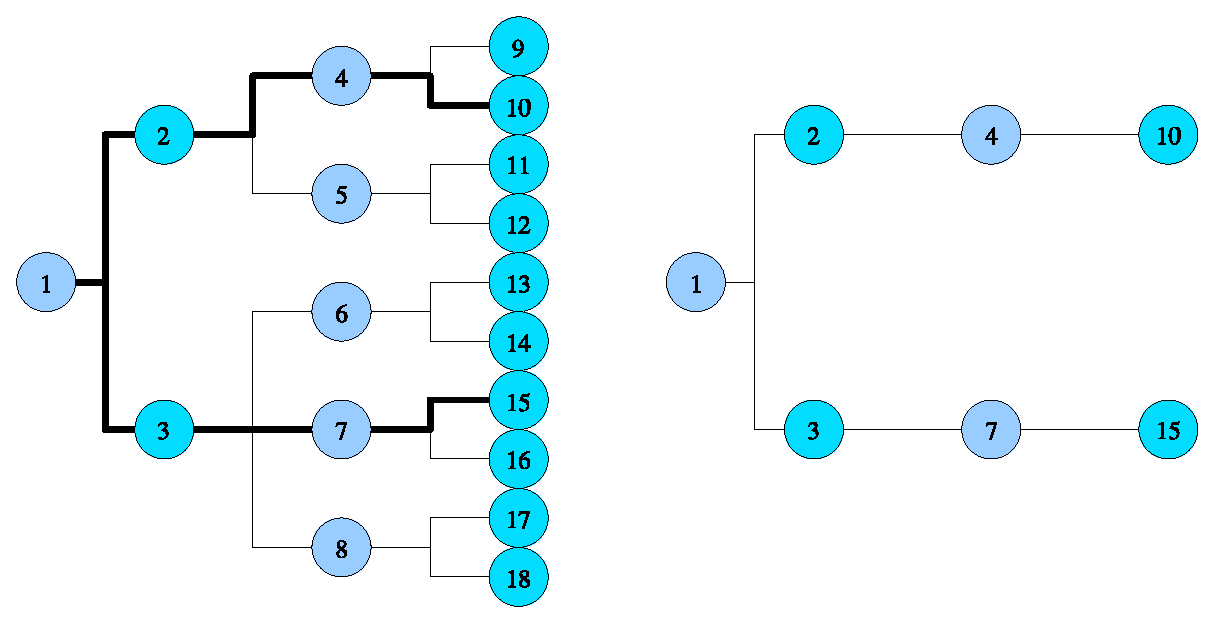
\includegraphics[scale=.6]{figures/redtree.eps}
    \caption{Complete tree and the reduced tree corresponding to the
             chosen scenarios (in bold).}
    \label{fig:Tree}
  \end{center}
  \vspace{-3ex}
\end{figure}

Each of the chosen nodes in the $k$-th stage now becomes the root of a 
branch of the tree, which we call a subtree. In each subtree we choose 
the scenario that minimises the distance to an average scenario in the 
same subtree.
%
Let $S_t$ be the set of nodes in the subtree $S$ at stage $t$, and 
$|S_t|$ its cardinality. For each stage $t$ within subtree $S$, 
we determine an artificial node $n_t$ by averaging the data 
associated to all nodes at this stage:
\[
n_t = \frac{1}{|S_t|} \sum_{l_t \in S_t} (T^{l_t}, W^{l_t}, h^{l_t}, q^{l_t}),
\quad k < t \le T.
\]

We define the average scenario for subtree $S$ as the ordered
set of nodes $s_k = \{ l_k, n_{k+1}, \ldots, n_T \}$.
Therefore, the average scenario $\bar s$ (in the complete tree) 
is obtained by listing the 
nodes from the root of the tree to the root of the subtree $S$, and 
then by appending the average nodes. We define it as
\[
\bar s = \{\, l_1, \ldots, l_k, n_{k+1}, \ldots, n_T \,\},
\]
where $l_t = a(l_{t+1})$ for $t = 1,\ldots, k-1$.
Scenario $\bar{s}$ is completely artificial, and there is no guarantee 
that it is feasible: therefore we cannot use it directly as our 
representative scenario. Instead, we use it as a reference point to 
which compare all other scenarios, and thus find the closest scenario 
among the existing ones: this way we do not introduce spurious 
infeasibilities. Hence, in the subtree $S$ we choose the 
representative scenario $s^*$ as 
%
\be  \label{repScenario}
   s^* = s_k, \quad k = \arg\min_{i\in S} \{ (1-p^i) D(s_i, \bar{s}) \},
\ee
%
where, since our ultimate goal is to find the most representative scenario in 
the subtree, we use the term $(1-p^i)$ to ``bring closer'' scenarios 
that have a higher probability of occurring.

We introduce the function $r(i): \Ctree \to \Rtree$ that maps each
node of the complete tree $\Ctree$ to a corresponding node in
the reduced tree $\Rtree$. Clearly, if $i \in \Rtree$, then
$i = r(i)$.
This mapping is used to decide how to initialise 
the warm-start iterate for the complete tree, as presented in the
next section. We remark that our generation process guarantees
that for each $i \in \Ctree$, the following properties hold:
\be  \label{eq:ReducedTreeProperties}
  a(r(i)) \in \Rtree, \quad \mbox{ and } \quad a(r(i)) = r(a(i)).
\ee

Continuing the example started above, we consider two subsets of 
scenarios, corresponding to nodes 9--12 (for the subtree rooted at 
node 2) and to nodes 13--18 (for the subtree rooted at node 3). Within 
each subset we build the scenario of average nodes and then find the 
representative scenario.
The resulting reduced tree is shown in the right of Figure~\ref{fig:Tree}.

It should be noted that the probabilities are normalised when 
the reduced tree is created, so that for each node the sum of the
conditional probabilities of visiting the children nodes is 1.
The conditional probability $\delta_R^k$ associated to node $k \in \Rtree$
is the sum of the conditional probabilities $\delta^i$ of the nodes 
$i \in \Ctree$ that are being replaced by node $k \in \Rtree$.
Defining $\mathcal{D}_{l_t} = \{ i \in \Ctree : a(i) = k \}$
the set of descendants of node $l_t$, and
$\mathcal{I}_k = \{\, i \in \Ctree : r(i) = k \,\}$, $k \in \Rtree$,
the set of nodes that are initialised by node $k$,
this can be written formally as
\be  \label{eq:UpdateCondProbs}
  \delta_R^k = \sum_{i \in \mathcal{I}_k \cap \mathcal{D}_{l_t}} \delta^i.
\ee

Remembering that the path probability $p^i$ is defined recursively as
$p^i = \delta^i p^{a(i)}$, equation~(\ref{eq:UpdateCondProbs}) is equivalent 
to updating the path probabilities $p^i$ as such:
\be  \label{eq:UpdatePathProbs}
  p^k_R = \sum_{i \in \mathcal{I}_k} p^i.
\ee

%
%
\subsection{Construction of the warm-start iterate}
\label{sec:Construction}

From the reduced tree we build the reduced deterministic 
equivalent problem
\be \label{eq:ReducedProblem}
\min\; c_R^T x_R \;\quad \mbox{s.t. }\; A_R x_R = b_R, \; x_R \ge 0,
\ee
with $A_R \in \R^{m_R\times n_R}$, $x_R \in 
\R^{n_R}$ and $b_R \in \R^{m_R}$. This problem is 
much smaller than the complete formulation, and hence we expect it to 
be much easier to solve.

We solve problem (\ref{eq:ReducedProblem}) with an interior point method. 
For the reasons presented in Section~\ref{sec:WarmStart}, we do not 
aim for optimality, but we stop at a sufficiently advanced barrier 
parameter $\mu^*_R$ corresponding to merely a few digits of accuracy in the 
solution. The primal--dual iterate, $(x_R^*,y_R^*,s_R^*)$, 
is used to generate the warm-start iterate for the complete problem.
However, the solution of the reduced problem needs to be expanded to the size 
of the complete problem before being used as a warm-start iterate.
In the construction phase we take into account the relationship
between the reduced and the complete trees.

The nodes that appear in the reduced tree directly provide a warm-starting
solution for the corresponding blocks; therefore, their parts of solution
can be copied over to initialise the complete iterate.
%
For the nodes of the complete tree which did not appear in the reduced 
tree, we look for a neighbouring node in the reduced tree. We find it 
by walking up the tree until we encounter a node that was in the reduced 
tree; at this point, we walk back down along the chosen scenario and return 
the index of a reduced tree node of the same stage as the original 
node.
Therefore, parts of the reduced-tree solution are replicated in the 
complete iterate. 

The blocks of the primal solution can be copied across directly.
The blocks of the dual solution must be rescaled according to probabilities
to guarantee dual feasibility in the expanded problem.
Let $(\hat x^{l}, \hat y^{l}, \hat s^{l})$ be the part of solution
of the expanded problem corresponding to node $l$. This is initialised
from the corresponding block of solution $(x_R^{l}, y_R^{l},  s_R^{l})$
of the reduced problem in the following manner:
\be  \label{eq:WarmstartSolution}
  \hat x^{l} = x_R^{r(l)}, \qquad 
 (\hat y^{l}, \hat s^{l}) = \frac{p^{l}}{p_R^{r(l)}} (y_R^{r(l)}, s_R^{r(l)}),
  \qquad l \in \Ctree,
\ee
where $p^i_R$ is computed according to (\ref{eq:UpdatePathProbs}).
This means that the dual reduced-tree solution is spread among the
nodes it initialises, as can be seen here:
\[
   \sum_{i \in \mathcal{I}_k} (\hat y^i, \hat s^i)
  = \sum_{i \in \mathcal{I}_k} \frac{p^i}{p^k_R} (y^k_R, s^k_R)
  = (y^k_R, s^k_R) \frac{1}{p^k_R} \sum_{i \in \mathcal{I}_k} p^i 
  = (y^k_R, s^k_R).
\]

Considering again the example of Figure~\ref{fig:Tree}, suppose that 
in the reduced tree we accepted only the scenarios that end at 
node 10 and node 15, so that the reduced tree consists of nodes 
1, 2, 3, 4, 7, 10 and 15. By solving the corresponding reduced problem, 
we obtain the parts of the solution vector associated to such 
nodes: these can be used directly in the complete iterate
(Figure~\ref{fig:Solution} top). 
We fill the missing elements 
by reproducing the solution from the nodes in the same subtree 
and the same stage (Figure~\ref{fig:Solution} bottom).
The proposed way of constructing the complete iterate is easy to
implement and its execution time is negligible.
%
\begin{figure}[ht]
  \begin{center}
    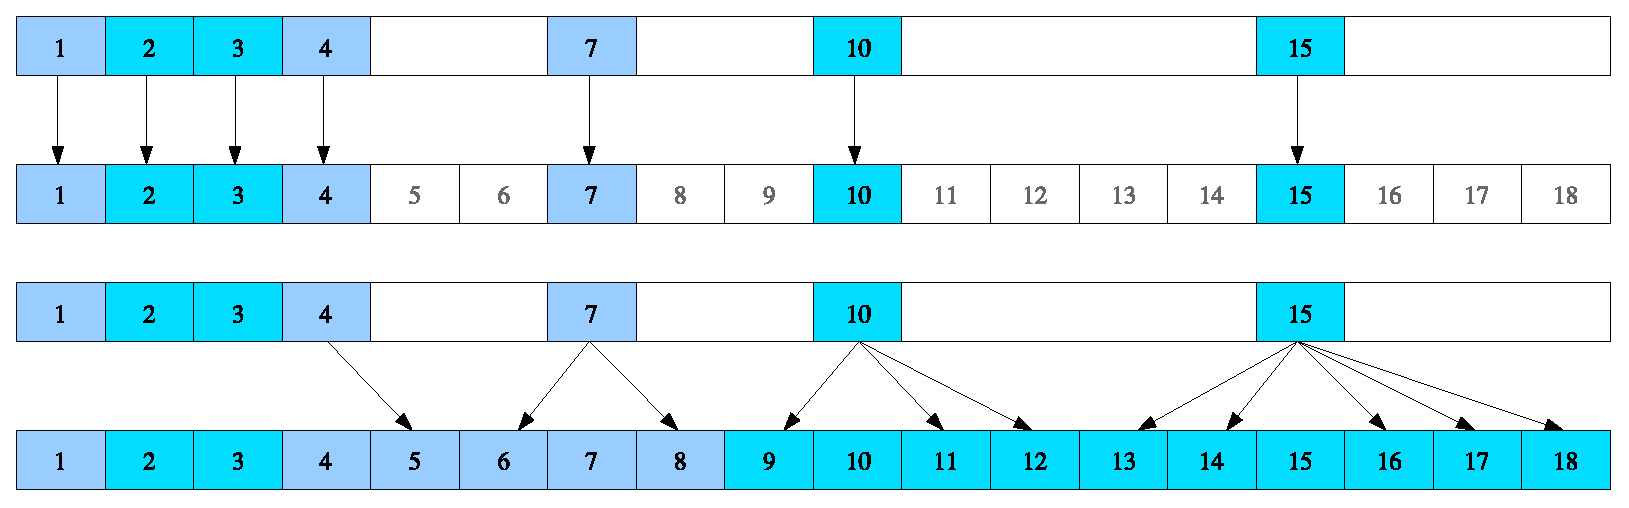
\includegraphics[scale=.51]{figures/solution.eps}
    \caption{Generation of the warm-start iterate.}
    \label{fig:Solution}
  \end{center}
  \vspace{-3ex}
\end{figure}

\ignore{
This simple strategies can be further 
generalised by considering a linear combination of the solutions 
corresponding to nodes that belong to the same stage. In this sense, 
the parts of the solution for nodes 4 and 7 may be used to initialise 
the solution for nodes 5, 6 and 8 (similarly for nodes 10 and 15 to 
initialise the starting solution for the other leaf nodes).
}

%
% Section
%
\section{Analysis of the warm-start iterate}
\label{sec:Analysis}

In this section we study how the warm-start iterate generated with 
the procedures presented above satisfies the conditions expressed by 
Gondzio and Grothey \cite{GondzioGrothey03}. 
Contrary to what is assumed in both \cite{YildirimWright} and 
\cite{GondzioGrothey03}, in our approach the dimension of the problem changes, 
as the reduced tree problem is, by construction, much smaller than the 
complete problem.

However, in a similar way as we did with the solution vector, 
we can expand our problem to one which has the same dimension 
as the complete problem (\ref{eq:CompleteProblem}) by replicating
the blocks in the coefficient matrix and in the objective and right-hand 
side vectors, as shown in Figure~\ref{fig:ExpandedSystem}.
%
\begin{figure}[ht]
  \begin{center}
    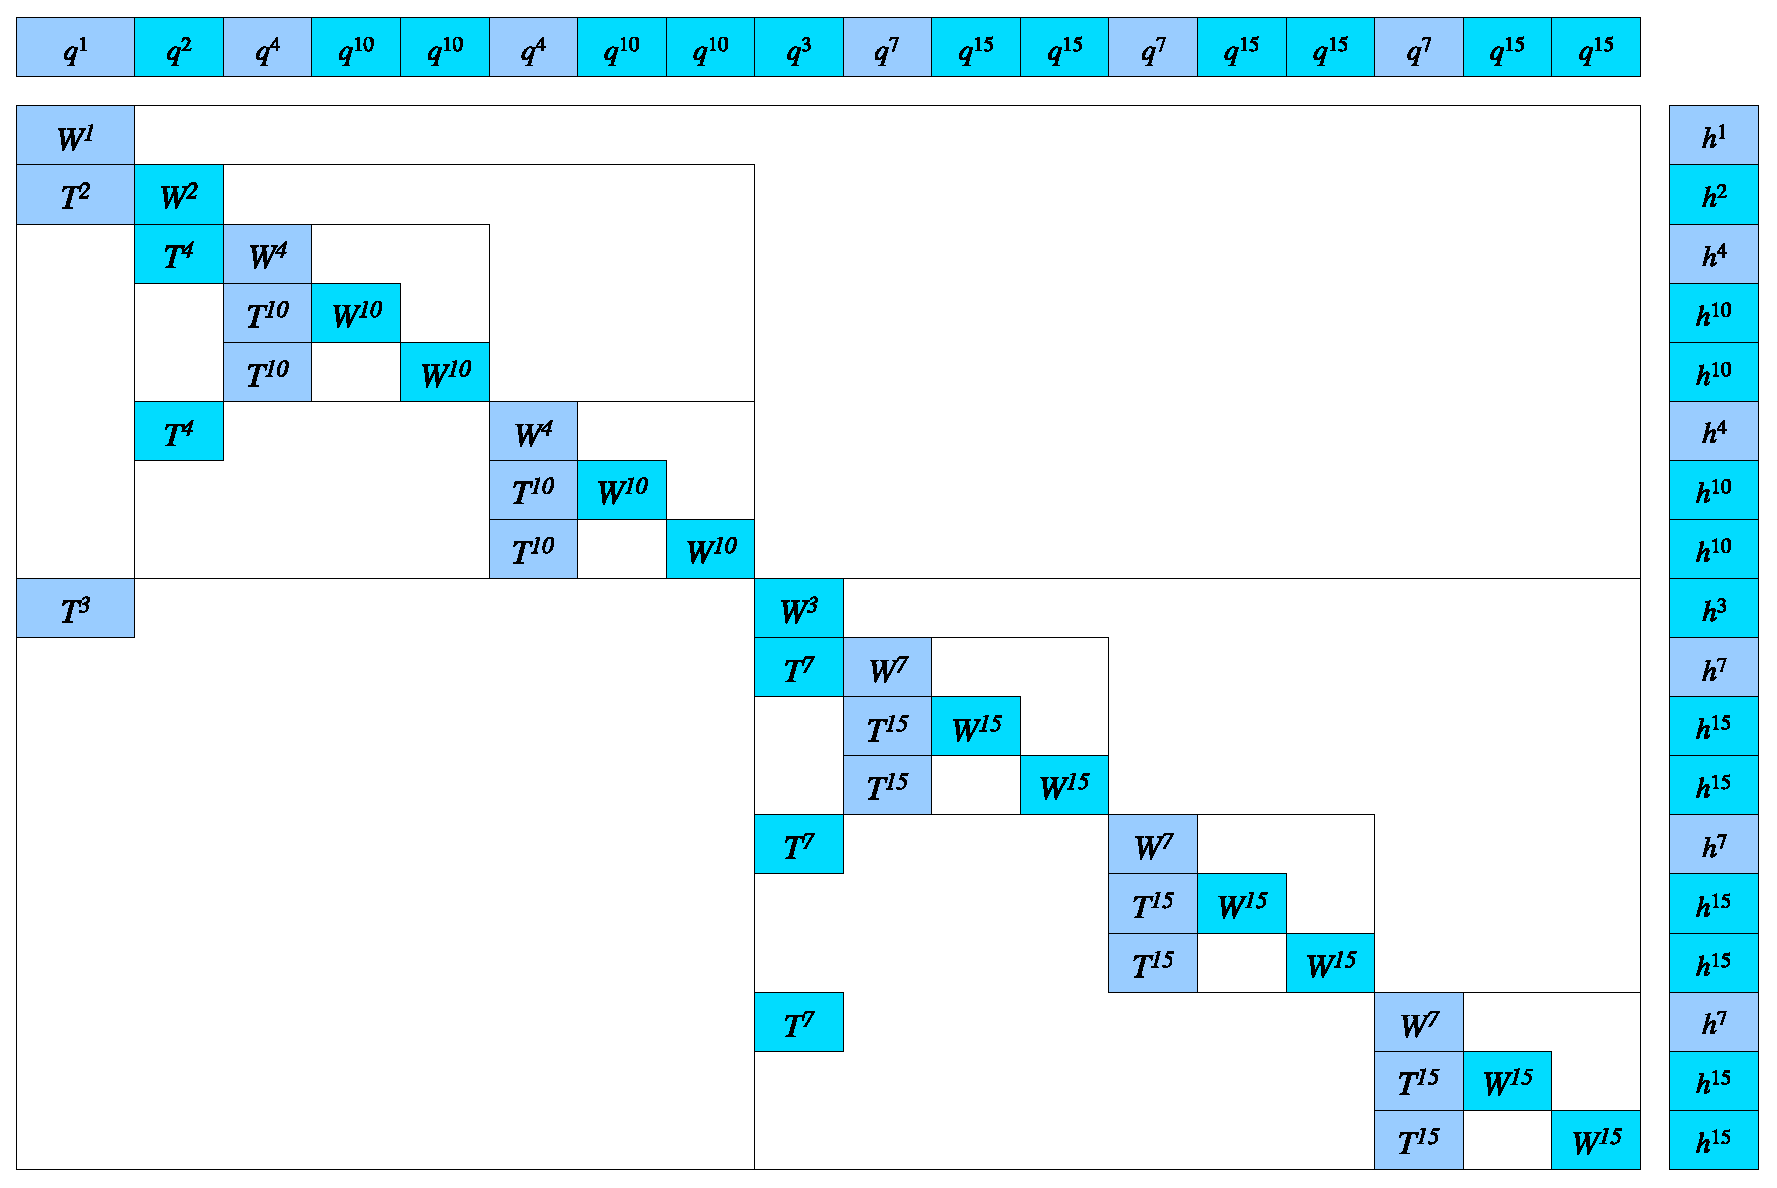
\includegraphics[scale=.50]{figures/expandedsystem.eps}
    \caption{The expanded system for the event tree of Figure~\ref{fig:Tree}.}
    \label{fig:ExpandedSystem}
  \end{center}
  \vspace{-3ex}
\end{figure}

This corresponds to creating the (artificial) expanded problem
\be \label{eq:ExpandedProblem}
\min\; \hat{c}^T x \;\quad \mbox{s.t. }\; \hat{A} x = \hat{b},
    \; x \ge 0,
\ee
the dimension of which, $\hat{A} \in \R^{m\times n}$, 
$\hat{c}, x \in \R^{n}$ and $\hat{b} \in \R^{m}$,
corresponds to the dimension of the complete problem 
(\ref{eq:CompleteProblem}).
%
Note that the warm-start iterate $(\hat{x},\hat{y},\hat{s})$
generated by the procedure of Section~\ref{sec:Construction}
is a solution to the expanded problem (\ref{eq:ExpandedProblem}) 
to the level of accuracy with which we solved the reduced problem.
This guarantees the following:
\be  \label{eq:ExpandedSolutionProperties}
\hat{A} \hat{x} = \hat{b}, \qquad
\hat{A}^T \hat{y} + \hat{s} = \hat{c}, \qquad
\hat{X} \hat{S} \approx \mu^*_R e.
\ee

In order to prove a feasibility result for the expanded problem,
we first need to prove a technical result.

\begin{lemma}  \label{th:SumOfTerms}
The following holds:
\[
\sum_{i \in \mathcal{D}_{l}} {T^{r(i)}}^T \hat y^i
  = \frac{p^{l}}{p^{r(l)}_R}\sum_{k \in \mathcal{D}_{r(l)}^R}
    {T^k}^T y^k_R.
\]
\end{lemma}
%
\begin{proof}
We have this chain of identities:
\[
\begin{split}
\sum_{i \in \mathcal{D}_{l}} {T^{r(i)}}^T \hat y^i
  &= \sum_{i\in\mathcal{D}_{l}} {T^{r(i)}}^T y^{r(i)}_R\frac{p^i}{p^{r(i)}_R}\\
  &= \frac{p^{l}}{p^{r(l)}_R}\sum_{i \in \mathcal{D}_{l}} {T^{r(i)}}^T
    y^{r(i)}_R \frac{\delta^i}{\delta_R^{r(i)}}\\
  &= \frac{p^{l}}{p^{r(l)}_R}\! \sum_{k \in \mathcal{D}_{r(l)}^R} \!\!
       \frac{{T^k}^T y^k_R}{\delta_R^k}
       \sum_{i \in \mathcal{I}_k \cap \mathcal{D}_{l}}\!\!\! \delta^{i},
\end{split}
\]
where we exploited the fact that
\(
  \mathcal{D}_{l} = \bigcup_{k \in \mathcal{D}_{r(l)}^R}
     \mathcal{I}_{k} \cap \mathcal{D}_{l}.
\)
The claim follows from (\ref{eq:UpdateCondProbs}).
\end{proof}

\begin{theorem}  \label{th:FeasibleReducedSolution}
If $(x_R, y_R, s_R)$ is primal and dual feasible for
the reduced problem (\ref{eq:ReducedProblem}),
then the warm-start solution (\ref{eq:WarmstartSolution}) is 
primal and dual feasible for the expanded problem (\ref{eq:ExpandedProblem}).
\end{theorem}
%
\begin{proof}
For the primal case, as $\hat x^{l} = x^{r(l)}_R$, this is trivially
satisfied:
\be  \label{eq:RedTreePrimalContribution}
   T^{r(l)}\hat x^{a(l)} + W^{r(l)} \hat x^{l} =  h^{r(l)}, 
      \quad l \in \Ctree.
\ee
%
For the dual case, by assumption the reduced problem solution satisfies 
the dual constraints:
\[
  {W^{r(l)}}^T y^{r(l)}_R +\sum_{i \in \mathcal{D}^R_{r(l)}} {T^{r(i)}}^T
     y^{r(i)}_R + s^{r(l)}_R = p^{r(l)}_R q^{r(l)},
     \quad r(l) \in \Rtree.
\]
Multiplying both terms by $p^{l}/p^{r(l)}_R$ we obtain
\[
  \frac{p^{l}}{p^{r(l)}_R} \Big( {W^{r(l)}}^T y^{r(l)}_R
     +\sum_{i\in \mathcal{D}_{r(l)}^R} {T^{r(i)}}^T y^{r(i)}_R + s^{r(l)}_R
     \Big) = p^{l} q^{r(l)},
\]
which, according to (\ref{eq:WarmstartSolution}) and 
Lemma~\ref{th:SumOfTerms}, becomes
\be  \label{eq:RedTreeDualContribution}
  {W^{r(l)}}^T \hat y^{l}+\sum_{i\in\mathcal{D}_{l}}{T^{r(i)}}^T \hat y^i
   + \hat s^{l} = p^{l} q^{r(l)}, \quad l \in \Ctree,
\ee
so $(\hat y, \hat s)$ satisfies
the dual constraints in the expanded problem.
\end{proof}

%
%
\subsection{Absorbing perturbations}

We argue that the difference between the data of the expanded 
problem (\ref{eq:ExpandedProblem}) and that of the original (complete) 
problem (\ref{eq:CompleteProblem}) can be interpreted as a perturbation 
between two problem instances of identical dimension. 
Clearly the expanded system has merely a theoretical
interest, as we use it to evaluate the magnitude of the 
perturbation introduced, and we never generate it in practice.

A warm-start strategy for interior point methods is successful only
under guarantee that this perturbation is small enough. The 
theoretical results of \cite{YildirimWright,GondzioGrothey03} provide 
bounds on the magnitude of the perturbation that can be absorbed 
in one interior point iteration. 
The analysis presented in \cite{GondzioGrothey03} concerns the case
where the search direction is split into primal and dual 
feasibility-restoring directions. 
We will give a more general result and apply it to the situation 
of warm start for stochastic programming problems.

We assume that a long-step path-following algorithm is used, 
and we work with the symmetric neighbourhood $\Nhood_s(\gamma)$
of the central path defined in (\ref{eq:SymmetricNeighbourhood}),
%
where $0 < \gamma < 1$. 
In the authors' experience, such a neighbourhood best describes the desired 
properties of a ``well-centered'' interior point iterate.
%
We consider the following Newton system:
\be \label{eq:NewtonSystem2}
\left[ \begin{array}{ccc}
    A & 0 & 0 \\ 0 &A^T & I \\ S & 0 & X
  \end{array} \right]
\left[ \begin{array}{c}
    \Delta x \\ \Delta y \\ \Delta s
  \end{array} \right] = 
\left[ \begin{array}{c}
    \xi_b \\ \xi_c \\ 0
  \end{array} \right],
\ee
the last equation of which implies
\[
 s_i\Delta x_i + x_i\Delta s_i = 0, \qquad i = 1, \ldots, n.
\]

Following the arguments of \cite{GondzioGrothey03}, the Newton
direction (\ref{eq:NewtonSystem2}) can be expressed in terms 
of the primal and dual residuals $\xi_b$, $\xi_c$ as
%
\begin{eqnarray}  \label{eq:Directions}
  \Delta x & \hspace{-1ex} = \hspace{-1ex} & 
  (XS^{-1} \! A^T (AXS^{-1} \!\! A^T)^{-1} \! AXS^{-1} \!\!-\!\! XS^{-1} )\xi_c
  \! + \! XS^{-1} \! A^T (AXS^{-1} \! A^T)^{-1} \xi_b, \nonumber \\
  \Delta y & \hspace{-1ex} = \hspace{-1ex} & 
  (AXS^{-1} A^T)^{-1} (AXS^{-1} \xi_c + \xi_b),                  \\
  \Delta s & \hspace{-1ex} = \hspace{-1ex} & 
  (I - A^T (AXS^{-1} \! A^T)^{-1} AXS^{-1} )\xi_c 
  \! - \! A^T (AXS^{-1} \! A^T)^{-1} \xi_b.            \nonumber
\end{eqnarray}

We consider the matrix
\[
  Q = I - S^{-1} A^T (A X S^{-1} A^T)^{-1} A X,
\]
and restate Lemma~3.2 of \cite{GondzioGrothey03},
which provides a bound on the norm of $Q$, in terms of
the symmetric neighbourhood $N_s(\gamma)$.

\begin{lemma}  \label{th:BoundQ}
If $w \in N_s(\gamma)$, then $\|Q\|_2 \le 1/\gamma$.
\end{lemma}
%
\begin{proof}
For a point $w \in N_s(\gamma)$, the following inequalities hold:
\[
  (x_i s_i)^{-1/2} \le (\gamma\mu)^{-1/2},
  \quad \mbox{ and } \quad
  (x_i s_i)^{1/2} \le (\mu / \gamma)^{1/2}.
\]
With some manipulations, we can express matrix $Q$ as
\[
Q = X^{-1/2}S^{-1/2} \left[ I - X^{1/2}S^{-1/2}A^T(AXS^{-1}A^T)^{-1}AX^{1/2}S^{-1/2} \right] X^{1/2}S^{1/2},
\]
where the term in square brackets is an orthogonal projection on the null
space of $AX^{1/2}S^{-1/2}$, so its Euclidean norm is 1.
As desired, we obtain
\[
  \| Q \|_2 = \| X^{-1/2}S^{-1/2} \|_2 \| X^{1/2}S^{1/2} \|_2 \le 1/\gamma.
  \qedhere
\]
\end{proof}

In the next Lemma we state sufficient conditions for the perturbations
to guarantee a full Newton step.

\begin{lemma}  \label{th:FullNewtonStep}
Let $w \in N_s(\gamma)$ be the current primal--dual iterate 
and define the scaled residuals 
\be
  \tilde \xi_b = X^{-1} A^T (A A^T)^{-1} \xi_b 
  \quad \mbox{ and } \quad 
  \tilde \xi_c = S^{-1} \xi_c.     \label{RelPerturbs}
\ee
If for $\beta < 1$ we have
\[
\|\tilde{\xi}_b\|_\infty + \|\tilde{\xi}_c\|_\infty 
    \le \beta\left(1 + \sqrt{n} / \gamma \right)^{-1},
\]
then the full Newton step (\ref{eq:NewtonSystem2}) from 
the current point is feasible.
\end{lemma}
%
\begin{proof}
Using the definitions of the matrix $Q$ and of the relative residual 
vectors (\ref{RelPerturbs}),
the relations (\ref{eq:Directions}) simplify to
\[
   X^{-1}\Delta x = -Q \tilde{\xi}_c + (I-Q) \tilde{\xi}_b = -S^{-1}\Delta s,
\]
%\begin{eqnarray*}
%   X^{-1}\Delta x & \!\! = \!\! & 
%       -Q \tilde{\xi}_c + (I-Q) \tilde{\xi}_b, \\
%   S^{-1}\Delta s & \!\! = \!\! & 
%        Q \tilde{\xi}_c - (I-Q) \tilde{\xi}_b, 
%\end{eqnarray*}
%
yielding the bound
%
\be  \label{boundx}
\|X^{-1}\Delta x\|_\infty
  \le \|Q\|_\infty\|\tilde{\xi}_c\|_\infty 
       + (1 + \|Q\|_\infty)\|\tilde{\xi}_b\|_\infty
  \le (1 +\|Q\|_\infty)(\|\tilde{\xi}_b\|_\infty + \|\tilde{\xi}_c\|_\infty).
\ee
%
As $(x,y,s)\in N_s(\gamma)$, using Lemma~\ref{th:BoundQ} we get
that $\|Q\|_\infty \le \sqrt{n} \|Q\|_2 \le \sqrt{n} / \gamma$.
Substituting it into (\ref{boundx}), we obtain
\[
\|X^{-1}\Delta x\|_\infty
   \le \left(1+\sqrt{n} / \gamma \right)(\|\tilde{\xi}_b\|_\infty 
       + \|\tilde{\xi}_c\|_\infty),
\]
which, under the condition of the Lemma, implies 
\begin{equation}  \label{eq:FullNewtonStep}
\|X^{-1}\Delta x\|_\infty = \|S^{-1}\Delta s\|_\infty \le \beta,
\end{equation}
that is the full Newton step is feasible, as $\beta < 1$.
\end{proof}

\begin{theorem}
Let $w \in \mathcal{N}_s(\gamma)$ and $\beta < 1$.
Under the conditions of Lemma~\ref{th:FullNewtonStep},
%The full Newton step in the direction $(\Delta x, \Delta y, \Delta s)$
%is feasible and 
the new point
$\bar w = (x + \Delta x, y + \Delta y, s + \Delta s)
\in \mathcal{N}_s(\frac{1-\beta^2}{1+\beta^2}\gamma)$.
\end{theorem}

\begin{proof}
At the new point $(\bar x, \bar y, \bar s)$ the barrier parameter is
\be  \label{eq:NewBarrier}
  n \bar\mu = \sum_{i=1}^n \bar x_i \bar s_i 
            = \sum_{i=1}^n (x_i +\Delta x_i)(s_i +\Delta s_i)
            = \sum_{i=1}^n (x_is_i + \Delta x_i\Delta s_i).
\ee
%
Using (\ref{eq:FullNewtonStep}) from Lemma~\ref{th:FullNewtonStep}, 
we have that
$\|X^{-1}\Delta x\|_\infty\|S^{-1}\Delta s\|_\infty \le \beta^2$,
and so
\be  \label{eq:BoundsDeltaxDeltas}
 -\beta^2x_i s_i \le \Delta x_i \Delta s_i \le \beta^2 x_i s_i;
\ee
by summing up all products we obtain
\[
 -\beta^2 n\mu \le \sum_{i=1}^n \Delta x_i \Delta s_i \le \beta^2 n\mu,
\]
which, by adding $n\mu = \sum_i x_i s_i$ to all terms and using 
(\ref{eq:NewBarrier}), leads to
\be  \label{eq:BoundsNewBarrier}
(1-\beta^2) n\mu \le n \bar \mu \le (1+\beta^2) n\mu.
\ee

We now study whether the new iterate is still in (some) symmetric
neighbourhood of the central path by checking the pairwise
complementary products
\[
\bar x_i \bar s_i = x_is_i + \Delta x_i\Delta s_i
                  = \left(1 +\frac{\Delta x_i\Delta s_i}{x_is_i} \right)x_is_i.
\]
Using (\ref{eq:BoundsDeltaxDeltas}) and (\ref{eq:BoundsNewBarrier}) 
we obtain
\begin{eqnarray*}
\bar x_i \bar s_i \ge (1-\beta^2)\gamma\mu \ge \frac{1-\beta^2}{1+\beta^2}\gamma\bar\mu, \\
\bar x_i \bar s_i \le (1+\beta^2)\frac{\mu}{\gamma} \le \frac{1+\beta^2}{1-\beta^2}\frac{1}{\gamma}\bar\mu,
\end{eqnarray*}
which proves the statement of the theorem.
\end{proof}

%
%
\subsection{Conditions on the warm-start iterate}

We use Lemma~\ref{th:FullNewtonStep} to obtain conditions that the 
reduced tree has to satisfy in order for a warm start of the complete problem 
to be successful. In order to prove this result, we need to assume that 
the primal--dual solution $(x_R^\ast, y_R^\ast, s_R^\ast)$ to the reduced 
stochastic programming problem is uniformly bounded, say,
%
\be  \label{xysBound}
  \max\{\|x_R^\ast\|_\infty, \|y_R^\ast\|_\infty, \|s_R^\ast\|_\infty\} \le B,
  \quad
  \max\{\|(X_R^\ast)^{-1}e\|_\infty,\|(S_R^\ast)^{-1}e\|_\infty\} \le B,
\ee
%
where $B>1$. 
It is worth noting that since we work with the symmetric neighbourhood
(\ref{eq:SymmetricNeighbourhood}), 
we actually need only the first inequality to hold.
Indeed, if $x_j^\ast \leq B$ then 
$1 / s_j^\ast \leq x_j^\ast / (\gamma \mu) \leq B / (\gamma \mu)$
and, similarly, if $s_j^\ast \leq B$ then 
$1 / x_j^\ast \leq s_j^\ast / (\gamma \mu) \leq B / (\gamma \mu)$.
In other words, the boundedness of the iterate 
$(x_R^\ast, y_R^\ast, s_R^\ast)$ implies the boundedness of the 
component-wise inverses of $x_R^\ast$ and $s_R^\ast$.

\ignore{
We argue that our way of constructing a reduced event tree by choosing
scenarios that minimize the distance from a representative average
scenario from each subtree can be designed to produce perturbations
which satisfy the assumptions of Lemma~\ref{th:FullNewtonStep}.
}

The reduced problem solution is in a neighbourhood of the central path 
for the reduced problem. In particular, this is the case if additional 
centering steps are computed once the desired tolerance level has been 
attained \cite{Gondzio98}. 
Since parts of this solution are copied to create the 
complete warm-start iterate, this will be centered as well.
Using the properties (\ref{eq:ExpandedSolutionProperties}),
the residuals for the complete problem at the warm-start point 
$(\hat{x}, \hat{y}, \hat{s})$ are:
\[
\begin{array}{lllll}
 \xi_b \!\!\! &=\; b-A\hat{x} \!\!&=&\!\! (b-\hat{b})-(A-\hat{A})\hat{x},\\
 \xi_c \!\!\! &=\; c -A^T\hat{y}-\hat{s}\!\! &=&\!\! (c-\hat{c})-(A-\hat{A})^T\hat{y},\\ 
 \xi_\mu\!\!\!&=\; \mu e - \hat{X}\hat{S}  & \approx & 0.
\end{array}
\]
%
It is crucial to ensure that the primal and dual residuals 
$\xi_b$ and $\xi_c$ are small. 
By construction, the elements of the vectors 
$(b-\hat{b})$ and $(c-\hat{c})$ that correspond to nodes in the reduced 
tree are zero; for the same reason, the corresponding blocks of 
$(A-\hat{A})$ are zero as well.
%
The elements corresponding to the nodes not considered in the reduced 
tree will be, in general, non zero. However, as the scenarios 
in the reduced tree were chosen according to (\ref{repScenario}) 
in order to minimize the distance 
from the average case, we expect the perturbations to be small. 

We can now state the following result.
%
\begin{lemma}  \label{th:BoundResiduals}
Let the reduced tree be chosen in such a way that for every node 
$i \in \Ctree$ the node distance (\ref{eq:Distance}) is 
$d(r(i), i) < \varepsilon$, for an $\varepsilon > 0$.
If the reduced problem solution is primal and dual feasible  
and satisfies (\ref{xysBound}), then
$\| \xi_b \|_{\infty} \leq \varepsilon B$
and  $\| \xi_c \|_{\infty} \leq \varepsilon B$.
\end{lemma} 
%
\begin{proof}
Using the form of the stochastic programming problem (\ref{DetEquiv})
we can write the primal residual of the complete problem as
\[
  \|\xi_b\|_\infty = \|b-A\hat x\|_\infty 
                   = \max\{\|h^{l} - T^{l}\hat x^{a(l)} 
                     - W^{l}\hat x^{l}\|_\infty:l = 1,\ldots,L_T\}.
\]
%
The contribution of a node $l \in \Ctree$ to $\xi_b$ is 
\[
\begin{split}
  \| \xi_b^{l} \|_{\infty}
    & = \|h^{l}\!-\!T^{l}\hat x^{a(l)}\!-\!W^{l}\hat x^{l}\| \\
    & = \|h^{l} \!-\! h^{r(l)} - (T^{l} \!- T^{r(l)})\hat x^{a(l)}
        - (W^{l} - W^{r(l)}) \hat x^{l}\| \\
%   & \le \|h^{l} \! - \! h^{r(l)}\| +
%         \|T^{l} \! - \! T^{r(l)}\| \| x^{a(r(l))}_R \|
%         + \|W^{l} - W^{r(l)}\| \| x^{r(l)}_R\| \\
    & \le \big( \|h^{l} \! - \! h^{r(l)}\| +
           \|T^{l} \! - \! T^{r(l)}\| +
           \|W^{l} \! - \! W^{r(l)}\| \big) B \\
    & \le  d(l, r(l)) B \le \varepsilon B,
\end{split}
\]
where the step from the first to the second line uses 
(\ref{eq:RedTreePrimalContribution}), and all norms here should be
intended as infinity norms.
%
This clearly implies that $\| \xi_b \|_\infty \le \varepsilon B$. 

The dual residual for the complete problem at the warm-start point 
can be written as
\[
  \|\xi_c\|_\infty = \|c -A^T\hat y -\hat s \|_\infty 
                   = \max\{\|p^{l}q^{l}
                   - {W^{l}}^T\hat y^{l} 
                   - \sum_{i \in \mathcal{D}_{l}} {T^{i}}^T\hat y^{i}
                   - \hat s^{l}
  \|_\infty : l = 1,\ldots,L_T\}.
\]
%
The contribution of a node $l \in \Ctree$ to $\xi_c$ is
\[
\begin{split}
  \xi_c^{l} 
 & = p^{l} q^{l} - {W^{l}}^T\hat y^{l}
     - \sum_{i\in \mathcal{D}_{l}} {T^i}^T \!\hat y^{i} -\hat s^{l} \\
 & = p^{l}(q^{l}\!-\! q^{r(l)})
     - (W^{l} \!-\! W^{r(l)})^T \hat y^{l}
     -\sum_{i \in \mathcal{D}_{l}} (T^{i} \!-\! T^{r(i)})^T\hat y^i \\
% & = p^{l}(q^{l} \!-\! q^{r(l)})
%     - \frac{p^{l}}{p^{r(l)}_R}(W^{l} \!-\! W^{r(l)})^T y^{r(l)}_R
%     -\sum_{i \in \mathcal{D}_{l}} (T^{i} \!-\! T^{r(i)})^T 
%           \frac{p^i}{p^{r(i)}_R} y^{r(i)}_R \\
 & = p^{l}(q^{l} \!-\! q^{r(l)})
     - \frac{p^{l}}{p^{r(l)}_R} \Big[
       (W^{l} \!-\! W^{r(l)})^T y^{r(l)}_R
       +\sum_{i\in \mathcal{D}_{l}} %\setminus\mathcal{D}_{r(l)}^R}
           (T^{i} \!-\! T^{r(i)})^T 
           \frac{\delta^i}{\delta^{r(i)}_R} y^{r(i)}_R \Big],
\end{split}
\]
where the step from the first to the second line uses 
(\ref{eq:RedTreeDualContribution}).
% and in the last line we 
%exploited the fact that $T^i - T^{r(i)} = 0$
%for $i \in \mathcal{D}_{l}\cap\mathcal{D}_{r(l)}^R$.
%
Taking norms (all norms here should be intended as infinity norms)
we obtain
\[
\begin{split}
  \| \xi_c^{l} \|_\infty
  & \le \|q^{l} - q^{r(l)}\| 
        + \|W^{l} - W^{r(l)}\| \| y^{r(l)}_R\|
        + \!\!\! \sum_{k\in \mathcal{D}_{r(l)}^R} \!\!\! \| y^{k}_R \| \!\!
          \sum_{i\in \mathcal{I}_k \cap \mathcal{D}_{l}\setminus \{k\} }
	  \!\!\! \| T^{i} - T^{k} \| \frac{\delta^i}{\delta_R^k} \\
  & \le \|q^{l} - q^{r(l)}\| 
        + \|W^{l} - W^{r(l)}\| \| y^{r(l)}_R\|
        + \!\!\! \sum_{k\in \mathcal{D}_{r(l)}^R} \!\!\! \| y^{k}_R \|
          \varepsilon \!\!
          \sum_{i\in \mathcal{I}_k \cap \mathcal{D}_{l}\setminus \{k\} }
	  \! \frac{\delta^i}{\delta_R^k} \\
  & \le \Big( \|q^{l} - q^{r(l)}\| 
        + \|W^{l} - W^{r(l)}\|
        + \!\!\! \sum_{k\in \mathcal{D}_{r(l)}^R} \!\!\!
	  \big( 1 - \frac{\delta^k}{\delta_R^k} \big) \varepsilon \Big) B \\
  & \le \varepsilon B\times 
        \max_{l} |\mathcal{D}_{l}^R| (1 - \frac{\delta^k}{\delta^k_R}).
        \qedhere
\end{split}
\]
%
%This clearly implies that $\| \xi_c \|_\infty \le \varepsilon B$. 
\end{proof}

The following result combines the findings of Lemmas~\ref{th:FullNewtonStep} 
and \ref{th:BoundResiduals}. 
%
\begin{theorem}  \label{th:Final}
Let the assumptions of Lemma~\ref{th:BoundResiduals} be satisfied and 
\[
\varepsilon B^2 \max\{\|A\|_\infty\|(AA^T)^{-1}\|_\infty, \; 1\} 
   \le \frac{1}{2} \left(1+\sqrt{n} / \gamma \right)^{-1}.
\]
Then the full Newton step (\ref{eq:NewtonSystem2})
from the warm-start iterate is feasible 
and it restores primal and dual feasibility.
\end{theorem}
%
\begin{proof}
Using the definition of $\tilde{\xi}_b$, we get
\[
\| \tilde{\xi}_b \|_{\infty} = \| X^{-1} A^T (AA^T)^{-1} \xi_b \|_{\infty} 
    \le
    \varepsilon B^2 \|A\|_{\infty} \|(AA^T)^{-1}\|_{\infty} 
    \le \frac{1}{2} \left(1+\sqrt{n} / \gamma \right)^{-1},
\]
and similarly for $\|\tilde{\xi}_c\|_{\infty}$.
Now the result follows from  Lemma~\ref{th:FullNewtonStep}. 
\end{proof}

A few remarks are in order about these results: first
Theorem~\ref{th:Final} implies that if we can choose the reduced
scenario tree such that $\varepsilon = \max_i\{d(r(i),i)\}$ small enough
to satisfy the bound given in the Theorem, then the warmstart
constructed from the reduced scenario tree will be successful for the
complete problem. Unfortunately we have only limited influence on
$\varepsilon$: indeed $\varepsilon$ is the result of the variation of
the problem data between the expanded and the complete system.
However, we can reduce $\varepsilon$ by having a
denser reduced tree, although this would make the solution of the
reduced problem more expensive.

\fb{
We can also play with $\mu$, not just $\epsilon$
}

It is important to remember, however,
that these are theoretical bounds. There is a gap between theory and
practice. In practice much larger infeasibilities 
$\|\tilde{\xi}_b\|, \|\tilde{\xi}_c\|$ can be absorbed. This is
confirmed by our numerical results where even choosing just 2
scenarios in the reduced tree leads to a significant reduction in the
number of interior point iterations required to solve the complete problem.


%
% Section
%
\section{Implementation and numerical results}
\label{sec:Results}

We first implemented the strategy of generating a reduced tree and 
the corresponding warm-start iterate within the \HOPDM \cite{Gondzio96} 
solver. We tested a series of publicly available stochastic problems in 
the SMPS format \cite{SMPS} coming from the POSTS collection 
available from:
\begin{center}
{\tt http://users.iems.northwestern.edu/\~{}jrbirge/html/dholmes/post.html}.
\end{center}
%
% while problem {\tt stocfor} comes from \\
% {\tt http://www.uwsp.edu/math/afelt/slptestset/download.html}. \\
%
It should be noted that we disabled presolve % and scaling 
in order to preserve the dimensions of the problems, and thus obtain 
sensible warm-start points.

We solved the reduced problem with an optimality tolerance of 
$5.0\times 10^{-1}$, while the optimality tolerance for the complete 
problem was set to $5.0\times 10^{-8}$. 
Computations were performed on a Linux PC with 3.0GHz Intel Pentium 
processor and 1GB of RAM.
In Table~\ref{table:hopdm} we report the dimensions of the problems 
in terms of the number of stages and scenarios for the complete 
tree, the number of iterations and the computing time (in seconds) 
with cold start and warm start. The latter includes the generation 
and solution of the reduced problem, and the construction of the 
warm-start iterate.

While the analysis of Section~\ref{sec:Analysis} is very conservative
in the estimates of the absorbable perturbations, in practice we noticed
that the reduced-tree warm-start strategy is effective even with
a much sparser tree than suggested from the theory.
In the warm-start case, the reduced tree was built with only 2 scenarios.

The instances solved show an overall good behaviour of our warm-start
strategy, with time savings up to 59\% for problem {\tt pltexpA5\_6}.
The generation of the reduced tree and the solution of the corresponding
problem (\ref{eq:ReducedProblem}) is generally fast, and as the problem 
sizes increase becomes negligible. However, for the smallest instances
of our test set ({\tt fxm2\_16}, {\tt fxm3\_6} and {\tt fxm4\_6}), it
is noticeable and consumes the savings produced by using an advanced
iterate.

\begin{table}[ht]
  \begin{center}
    \begin{tabular}{|l|r|r||r|r||r|r|} \hline
      \multicolumn{3}{|c||}{Problem data}&\multicolumn{2}{c||}{Cold start}&\multicolumn{2}{c|}{Warm start}\\
      \multicolumn{1}{|c|}{Name} & Stages & Scens & Iters & Time & Iters & Time \\ \hline \hline
fxm2\_16     &  2 &   16 &  22 &   1.2 & 13 &   1.0 \\
fxm3\_6      &  3 &   36 &  30 &   1.5 & 17 &   1.3 \\
fxm3\_16     &  3 &  256 &  40 &  31.1 & 20 &  20.7 \\
fxm4\_6      &  4 &  216 &  30 &   8.2 & 22 &   8.3 \\
fxm4\_16     &  4 & 4096 &  41 & 218.3 & 27 & 182.6 \\ \hline
%\hline
pltexpA3\_16 &  3 &  256 &  26 & 153.8 & 14 &  87.8 \\
pltexpA4\_6  &  4 &  216 &  36 &  55.8 & 16 &  27.5 \\
pltexpA5\_6  &  5 & 1296 &  81 & 772.0 & 30 & 311.5 \\ \hline
% \hline
storm27      &  2 &   27 &  41 &  95.4 & 22 &  53.2 \\
storm125     &  2 &  125 &  73 & 107.3 & 36 &  69.1 \\
storm1000    &  2 & 1000 & 107 &1498.3 & 45 & 831.5 \\ \hline
% \hline
% stocfor2     &  2 &   64 &  19 &   0.9 & 18 &   1.1 \\
% stocfor3     &  7 &  512 &  29 &   4.0 & 24 &   4.2 \\ \hline
    \end{tabular}
    \caption{Results obtained with \HOPDM, 2 scenarios in the reduced tree.}
    \label{table:hopdm}
  \end{center} \vspace{-3ex}
\end{table}

%
%
\subsection{Telecommunication problems}

Given the favourable results, we implemented the same approach 
in \OOPS \cite{GondzioSarkissian,GondzioGrothey04}, where we were 
able to test larger instances. 
Since \OOPS does not have features such as presolve and scaling,
% or freedom in the choice of the pivot elements. 
the accuracy requested in the solution has to be smaller. We set it to
$5.0 \times 10^{-4}$ which is more than enough for telecommunication
applications anyway.
On the other hand, \OOPS makes an effective use of its structure-exploiting
capabilities \cite{GondzioSarkissian,GondzioGrothey04},
allowing the solver to tackle large-scale problems 
and provides access to parallel computing techniques.

We applied our warm-start strategy to the capacity assignment problem 
with uncertain demand, a model relevant to the telecommunication 
industry \cite{Ouorou}. The objective of this model is to find 
the optimal choice of capacities to be assigned to the links 
in the network in order to minimize the unsatisfied customer demands.
In our particular application we assume that the topology 
of the network and the sets of origin--destination pairs are given 
and are not going to change during the planning horizon.

We model this situation as a two-stage stochastic linear program 
with recourse. The general model has the following form:
\[
  \min_x \; E_d [f(x,d)] \;\quad 
  \mbox{s.t. }\; \sum_{l \in {\cal A}} c_l x_l \le M, \;\;  x \ge 0,
\]
where $c_l$ and $x_l$ are the cost and the capacity of link $l \in {\cal A}$, 
respectively, and $M$ is a bound on the budget. The objective 
here is to minimize the expected cost (conditional on the uncertain 
demand). This general model describes the first stage 
decision about the link capacities.
The function $f(x,d)$ is defined in the following model, which 
describes the second stage decisions:
\[
\begin{array}{rll}
  f(x,d) =\min & \displaystyle\sum_{k\in {\cal D}} (d_k -\sum_{p\in P_k} z_p)\\
  \mbox{s.t.}  & \displaystyle\sum_{k\in {\cal D}} \sum_{p\in {\cal P}_k: l\in p} z_p \le x_l
                                        & \forall l \in {\cal A} \\
               & \displaystyle\sum_{p\in {\cal P}_k} z_p \le d_k
                                        & \forall k \in {\cal D} \\
               & z_p \ge0,
\end{array}
\]
where $d_k$ is the demand for the $k$-th origin--destination pair, 
$\mathcal{P}_k$ is a given set of paths linking the $k$-th pair, and $z_p$ 
is the flow on path $p$.

To generate the uncertain demands of each scenario 
we used the approach described in \cite{Ouorou}. 
For each origin--destination pair $k$ we need to have a demand 
estimate $d_k$, which can be determined from historic data 
or from an educated guess. The demand is assumed to be uniformly 
distributed around this estimate. Hence, the demand $d_k^s$ 
for the $k$-th pair in scenario $s$ is given by
\[
d_k^s = (1+ \epsilon_k^s)d_k,
\]
where $\epsilon_k^s$ is a random number generated in the interval 
$[-\rho, \, \rho]$. The value of $\rho > 0$ determines the range 
in which we assume the demand to fluctuate.
In our experiments we chose a value of $\rho = 0.5$, thus allowing
very large variations in the demand.
%
% This way of generating random scenarios provides us with an obvious 
% strategy of creating the reduced tree, that is by considering 
% the scenario corresponding to the given demand estimates.

The relevant network characteristics of the problems solved are shown 
in Table~\ref{table:ProblemData}, where we detail the size of the network, 
the number of demands considered, the overall number of paths and the
average number of arcs in each path.
%
%
% Names changed: 26.08.2006 (Jacek)
% minoux     mnx
% jll-gva    jlg
% magnantiA  mgntA
% T1mgnB     mgntB
%
\begin{table}[ht]
  \begin{center}
    \begin{tabular}{|l||r|r|r|r|r|} \hline
      Name      & Nodes & Arcs & Demands & Paths & Av.Length \\ \hline\hline
      mnx       &    12 &   50 &     66  &   189 & 2.6 \\
      jlg       &    26 &   84 &    264  &   697 & 5.6 \\
      mgntA     &    53 &  158 &   1378  &  3574 & 6.7 \\
      mgntB     &    70 &  210 &   2346  &  6137 & 6.4 \\ \hline
    \end{tabular}
    \caption{Characteristics of the telecommunication problems.}
    \label{table:ProblemData}
  \end{center} \vspace{-3ex}
\end{table}

\noindent For a problem with $N$ scenarios, the number of constraints and 
decision variables (including slacks) are
\[
m = 1 + N \times (\#{\cal A} + \#{\cal D}), \quad \mbox{ and } \quad
n = 1 + \#{\cal A} + N \times (\#{\cal A} + \#{\cal D} + \#{\cal P}),
\]
respectively, where $\#{\cal A}$ is the number of arcs, $\#{\cal D}$ 
the number of demands, and $\#{\cal P}$ the total number of paths.

In the second and third column of Table~\ref{table:oops} 
we report the solution statistics for \OOPS.
Computations were performed on a Linux PC with 3.0GHz Intel Pentium
processor and 2GB of RAM.
% We report the number of iterations and 
% the solution time for cold start and warm start cases.
In all cases the reduced tree was built with merely two scenarios.
Therefore the computation time corresponding to the solution 
of the reduced problem (included in time reported in the table) 
was always negligible. The savings of warm start over cold start 
strategy vary between 40\% and 80\% in most cases.
%
\begin{table}[ht]
  \begin{center}
    \begin{tabular}{|l||rr|rr||rr|rr|} \hline
     \multicolumn{1}{|c||}{\raisebox{-1ex}{Problem}} &
     \multicolumn{2}{c|}{Cold start} &
     \multicolumn{2}{c||}{Warm start} &
     \multicolumn{2}{c|}{Cold start} &
     \multicolumn{2}{c|}{Warm start}\\
              &Iters &   Time &Iters &   Time & Iters &   Time & Iters &   Time  \\ \hline\hline
mnx-100       &   15 &    6.7 &    9 &    3.9 &  15 &    3.9 &   9 &    2.6 \\
mnx-200       &   13 &   12.9 &    7 &    7.3 &  13 &    4.6 &   7 &    3.5 \\
mnx-400       &   16 &   28.9 &    8 &   15.5 &  16 &   10.5 &   8 &    6.3 \\
mnx-800       &   17 &   58.8 &   10 &   39.5 &  17 &   18.8 &  10 &   10.7 \\
mnx-1600      &   19 &  131.1 &   10 &   68.8 &  19 &   50.3 &  10 &   31.4 \\
\hline
jlg-100       &   21 &   38.3 &    6 &   15.5 &  21 &   11.0 &   6 &    6.1 \\
jlg-200       &   45 &  164.9 &   17 &   39.5 &  45 &   49.9 &  17 &   20.7 \\
jlg-400       &   44 &  255.2 &   18 &  103.1 &  43 &   83.2 &  19 &   39.7 \\ % EXC (Changed Jacek)
jlg-800       &   27 &  353.4 &   10 &  152.9 &  29 &  130.5 &  10 &   50.1 \\ % less aggressive
jlg-1600      &   32 &  855.3 &   13 &  360.6 &  35 &  286.1 &  14 &  129.7 \\ % less aggressive
\hline
mgntA-100     &   28 &  260.0 &   14 &  156.2 &  28 &   76.9 &  14 &   51.6 \\
mgntA-200     &   50 &  877.1 &   35 &  690.6 &  50 &  256.4 &  34 &  195.3 \\
mgntA-400     &   40 & 1470.3 &   14 &  572.5 &  40 &  410.9 &  14 &  181.6 \\
\hline
mgntB-100     &   23 &  511.1 &   14 &  318.0 &  23 &  137.5 &  14 &  103.9 \\
mgntB-200     &   25 &  909.4 &    8 &  332.4 &  25 &  284.2 &   8 &  140.5 \\
mgntB-400     &   29 & 2154.5 &    7 &  538.1 &  29 &  605.5 &   7 &  211.6 \\
\hline
    \end{tabular}
    \caption{Efficiency of the warm-start strategy in \OOPS in the serial
             case (2 scenarios in the reduced tree) and in the parallel case
	     (4 processors and 4 scenarios in the reduced tree).}
    \label{table:oops}
  \end{center} \vspace{-3ex}
\end{table}


We have also solved the smallest instances of these problems 
with Cplex~9.0 Barrier Solver. The problems 
{\tt mnx-100}, {\tt jlg-100}, {\tt mgntA-100} and {\tt mgntB-100} 
were solved in 1.1s, 7.1s, 4379.9s and 9030.4s, respectively.
This means that Cplex was about 4 and 2 times faster than \OOPS
on {\tt mnx-100} and {\tt jlg-100} problems, respectively 
but it was about 28 times slower than \OOPS on more difficult
{\tt mgntA-100} and {\tt mgntB-100} problems.

In the fourth and fifth columns of Table~\ref{table:oops} 
we report the parallel performance 
of \OOPS on a cluster of four machines with a 3.0GHz Intel Pentium 
processor and 2GB of RAM each.
In this case, we choose the size of the reduced tree to be equal 
to the number of processors employed for two complementary reasons: 
first, it is preferable to assign to \OOPS a balanced number of blocks 
on each processor, so we needed to guarantee that each processor 
gets at least one block; second, we obtain a more refined 
starting solution at no additional computational cost. 
However the analysis of the parallel results collected 
in Table~\ref{table:oops}
indicates that the use of a slightly larger reduced tree does not 
translate into any noticeable improvement in the warm start runs 
as measured with the number of warm start iterations.
Obviously, the solution times are reduced but this is the effect 
of using more processors.

%
% Section
%
\section{Other stuff}

\begin{itemize}
\item The reduced tree approach to construct a warmstart iterate 
doesn't seem to be IPM specific, and could be exploited also by a 
simplex solver (in which case, how would such a solver obtain the 
complete basis?). However, interior point methods have the advantage
of solving huge scale problems, parallelism, and extension to 
quadratic problems.

\item Provide a comparison between initial infeasibilities 
produced by Mehrotra's heuristic and the reduced-tree starting 
point. It would be great to have some sort of theoretical back-up 
about the relationship between magnitude of perturbation and 
initial infeasibilities.

\item Point out that the way we generate our starting point 
guarantees better centrality (at least in the sense of 
complementary pairs). Possibly this could be compared again 
with the points generated by Mehrotra's starting point heuristic.

\item Point out that if we knew about the underlying 
stochastic process, then we could exploit it directly in the 
generation of the reduced tree (althogh, in such a case how 
could we ensure the correspondence of nodes between the reduced 
and the complete tree?)

\item Clarify the issue of nonanticipativity constraints: 
since we have our own deterministic equivalent generator, we 
already avoid duplication without using those constraints.

Nonanticipativity means that the decisions taken at any stage 
do not depend on future realizations of the random parameter or 
on future decisions, but only on the history.

\item Mention that if the iterate produced by a reduced tree 
is not good enough (according to what criteria?), another one 
can be produced by generating a modified reduced tree (more 
bushy for example).
\end{itemize}

In our approach, the size of the problem changes in both 
the number of constraints and the number of variables in the 
primal and in the dual. Therefore, we are faced with the 
challenge of using the solution of the small instance to 
provide a warm-start iterate for the complete system. This 
entails initialising both the primal and the dual vectors, of 
which only a fraction of the elements are known. This objective 
can be achieved by exploiting the inherent structure of the problem.


\chapter{Conclusions}
%Started on 5 February 2007
%Mar: 31
%Apr:  1

%
% Chapter: Conclusions
%
\label{ch:Conclusions}

The relative youth of interior point methods means that there is still
a lot to learn and try, particularly in practical implementations.
We present here some observations derived from the experience
gathered during this research.

As we have seen in Chapter~\ref{ch:Correctors}, many attempts
have been made to find new and original search directions.
We believe that the direction generated from the Newton system,
possibly complemented by Mehrotra's second-order correction,
are only one of the possibility of exploring the solution space.

From the study of subspace searches explored in
Section~\ref{sec:SubspaceSearches}, it is clear that the more 
directions we consider, the better the final search direction 
we get. Therefore, if we had a cheap way of generating search
directions (rather than from solving a system of linear equations),
then these should be employed.
In this respect, Mehrotra and Li \cite{MehrotraLi} 
mention employing previous search directions alongside the usual ones. 
The use of these incurs an increased memory usage 
in order to store them, but no additional computational cost.
However, it does not seem that they were actually employed in
their implementation.
This opens some questions on what constitutes a valid
previous direction (only affine scaling, the final composite direction
or something else).

The analysis of Jarre and Wechs discussed in Section~\ref{sec:JarreWechs}
makes it very clear that the choice of the target $t$ in
the right-hand side of the Newton system is the driving
tool in finding effective search directions.
In our reimplementation of multiple centrality correctors, we
have pushed the target vector of complementary points further
in the infeasible space with the aim to generate a better
correction to the current iterate.

A big avenue of research, according to the author, is the development
of specialised techniques to exploit the problem structure.

This means that the development and diffusion of structure-exploiting
codes and of structure-aware modelling languages may become a necessary
requirement for a new generation of interior point codes.

In this sense, also theoretical developments in these aspects are 
wanted and necessary.


%
% Appendix
%
%\appendix
%\chapter{}\label{App_Chapter}
%\input{appendix}

%
% Bibliography
%
%\input{nocites}
\bibliographystyle{plain}
\bibliography{bibliography}

%
% End
%
\end{document}
